%========= File containing the main LaTex document ========%

\documentclass[]{./tpl/isipfe}
\graphicspath{{./img/}}

\input{./tpl/new_commands}

\makeindex

\begin{document}
    %=== File containing Global Configuration of the report ===%
%                                                          %
% Copyright (C) ISI - All Rights Reserved                  %
% Proprietary                                              %
% Written by Med Hossam <med.hossam@gmail.com>, April 2016 %
%                                                          %
% @author: HEDHILI Med Houssemeddine                       %
% @linkedin: http://tn.linkedin.com/in/medhossam           %
%==========================================================%

%============= Config new columns type ==============%
\newcolumntype{L}{>{\raggedright\arraybackslash}l}
\newcolumntype{R}{>{\raggedleft\arraybackslash}r}
\newcolumntype{C}{>{\centering\arraybackslash}c}
%==================================================%

%========= Config the cover section ==========%

\title{Conception et D\'eveloppement d'une Plateforme Web de Reconnaissance de Surface d'Attaque avec G\'en\'eration de Rapports Assist\'ee par IA et Int\'egration DevSecOps}

\author{Aymen AZIZI}

\diplomaName{Dipl\^ome National d'Ing\'enieur en Sciences Appliqu\'ees et Technologiques}
\speciality{S\'ecurit\'e des Syst\`emes Informatiques et R\'eseaux (SSIR)}

%% Encadrant professionnel
\proFramerName{M. Ali DORBOZ}
\proFramerSpeciality{Directeur Technique (CTO)}

%% Encadrante académique
\academicFramerName{Mme Sonia BEN AISSA}
\academicFramerSpeciality{Encadrante Universitaire}

%% Entreprise d'accueil
\companyName{Designet Web Agency}

%% Année universitaire
\collegeYear{2025 - 2026}

%%%%%% Signatures section %%%%%%

\proSignSentence{J'autorise l'\'etudiant \`a d\'eposer son rapport de projet de fin d'\'etudes en vue de la soutenance.}

\academicSignSentence{J'autorise l'\'etudiant \`a d\'eposer son rapport de projet de fin d'\'etudes en vue de la soutenance.}

%%% FR
\frenchAbstract{Ce projet de fin d'\'etudes porte sur la conception et le d\'eveloppement d'une plateforme web semi-agentique de reconnaissance de surface d'attaque, int\'egrant une corr\'elation par graphe de connaissances, une g\'en\'eration de rem\'ediations (\textit{Remediation-as-Code}) assist\'ee par IA locale contrainte, et une cha\^ine de livraison DevSecOps s\'ecuris\'ee. R\'ealis\'ee au sein de Designet Web Agency, la plateforme orchestre cinq microservices Python (reconnaissance, s\'ecurit\'e offensive, OSINT, IA, passerelle API) et un worker asynchrone pilot\'e par Redis Streams, le tout coordonn\'e par un back-end en Laravel 11. Le syst\`eme mod\'elise la surface d'attaque sous la forme d'un graphe relationnel (\textit{Asset $\rightarrow$ Port $\rightarrow$ Service $\rightarrow$ Vuln\'erabilit\'e $\rightarrow$ Impact}) stock\'e dans PostgreSQL 16 avec l'extension Apache AGE, avec calcul algorithmique du rayon d'impact (\textit{blast radius}) via NetworkX. L'IA locale, bas\'ee sur Ollama (\texttt{qwen2.5-coder}), contribue \`a pr\'eserver la confidentialit\'e des donn\'ees en \'evitant leur transmission \`a un fournisseur externe de LLM, et contribue \`a r\'eduire le risque d'hallucination en imposant des sorties structur\'ees et des citations directes vers les journaux bruts. La cha\^ine DevSecOps int\`egre des barri\`eres bloquantes (SAST, SCA, SBOM CycloneDX avec Syft, scan d'images Trivy et signature Cosign). L'application d'un cadre l\'egal strict (Proof of Authorization -- PoA) et de profils d'audit adaptatifs garantit une ex\'ecution s\'ecuris\'ee et non destructive.}

\frenchAbstractKeywords{Cybers\'ecurit\'e, Reconnaissance de surface d'attaque, Graphe de connaissances, Remediation-as-Code, DevSecOps, Redis Streams, PostgreSQL, Apache AGE, NetworkX, Ollama, Laravel 11, Flask, SBOM, Cosign}

%%% EN
\englishAbstract{This graduation project focuses on the design and development of a semi-agentic web platform for security attack surface reconnaissance, integrating knowledge graph correlation, constrained local AI for Remediation-as-Code generation, and an automated secure DevSecOps pipeline. Conducted at Designet Web Agency, the platform orchestrates five Python microservices (reconnaissance, offensive security, OSINT, AI, API gateway) and an asynchronous event-driven worker via Redis Streams, coordinated by a Laravel 11 back-end. The system models the attack surface as a knowledge graph (Asset $\rightarrow$ Port $\rightarrow$ Service $\rightarrow$ Vulnerability $\rightarrow$ Impact) stored in PostgreSQL 16 with Apache AGE, calculating blast-radius propagation via NetworkX. The local AI, powered by Ollama (qwen2.5-coder), preserves data privacy by preventing sensitive telemetry from being transmitted to third-party providers, while mitigating hallucination risks through structured JSON outputs and verifiable log citations. The DevSecOps pipeline enforces automated security gates (SAST, SCA, CycloneDX SBOM with Syft, Trivy container scans, and Cosign image signatures). A mandatory Proof of Authorization (PoA) validation ensures strict compliance with legal and ethical security auditing standards.}

\englishAbstractKeywords{Cybersecurity, Attack Surface Reconnaissance, Knowledge Graph, Remediation-as-Code, DevSecOps, Redis Streams, PostgreSQL, Apache AGE, NetworkX, Ollama, Laravel 11, Flask, SBOM, Cosign}

\setboolean{wantToTypeCompanyAddress}{false}
\companyEmail{contact@designet.tn.com}
\companyTel{27 180 092}
\companyFax{27 180 092}
\companyAddressAR{نهج الثورة - منزل تميم 8080}

    
    \frontmatter
        
%== It's advised to not modify the content of this file ===%
% To set your information, go to global_config.tex file    %
%==========================================================%

\thispagestyle{cover}%
\newgeometry{bottom=25mm,left=20mm,top=15mm,right=20mm}
\hspace{-47pt}
\begin{minipage}[l]{0.2\columnwidth}
\vspace{6mm}

\includegraphics[width=1.1\columnwidth]{img/tekup.png}\\
\end{minipage}
\hfill
\begin{minipage}[l]{0.6\columnwidth}
\centering
\footnotesize
\textbf{{R\'epublique Tunisienne}}\\
\vspace{1.5mm}
\textbf{{Minist\`ere de l'Enseignement Sup\'erieur\\
et de la Recherche Scientifique}}\\
\vspace{1.5mm}
%\textbf{{Université de Tunis El Manar}}\\
\vspace{1.5mm}
\textbf{{\'Ecole Sup\'erieure Priv\'ee de Technologies et d'Ing\'enierie}}\\
\vspace{1.5mm}
\textbf{{TEK-UP}}\\
\vspace{1.5mm}
\end{minipage}
\hfill
\begin{minipage}[l]{0.02\columnwidth}
\end{minipage}
\hfill
\begin{minipage}[l]{0.2\columnwidth}
\vspace{6mm}

\includegraphics[width=1.3\columnwidth]{img/logoSociete.png}\\
\end{minipage}
\vskip1.5cm

\begin{center}
{\LARGE{\textbf{\textsc{Rapport de Projet de Fin d'\'Etudes}}}}\\
\vskip0.5cm
\large

{\textbf{Pr\'esent\'e en vue de l'obtention du}}\\
\vskip2mm
{\textbf{\@diplomaName}}\\
{\textbf{Sp\'ecialit\'e : \@speciality}}\\
{}
\end{center}

\begin{center}
\textrm{\'Elabor\'e par :}\\
\vskip0.3cm
{\ifthenelse{\boolean{isBinomal}}
    {% IF TRUE
        \begin{center}
            \large\textbf{\@author}~~~~~ et ~~~~~
            \large\textbf{\@secondAuthor}
        \end{center}
    }
    {\Large\textbf{\@author}}% FALSE
}
\vskip12mm

\definecolor{isiBlue}{RGB}{31, 78, 121}

\begin{changemargin}{-9mm}{0cm}
\begin{minipage}[l]{1.1\columnwidth}
\begin{tcolorbox}[colframe=isiBlue,colback=white,boxrule=0pt,toprule=3pt,bottomrule=3pt,arc=0pt,top=0mm,right=0mm,left=0mm,bottom=0mm,boxsep=0.5mm]{
    \begin{tcolorbox}[colframe=isiBlue,colback=white, boxrule=0pt,toprule=1pt,bottomrule=1pt,arc=0pt,enlarge bottom by=-0.9mm, auto outer arc]
        \centering
        {\huge\textbf{\@title}}
    \end{tcolorbox}
}
\end{tcolorbox}
\end{minipage}
\end{changemargin}

\end{center}
\vskip8mm%

\begin{center}
\large
\begin{minipage}[c]{0.30\columnwidth}
Encadrant Professionnel :\\
Encadrante Universitaire :
\end{minipage}
\hfill
\begin{minipage}[c]{0.40\columnwidth}
\textbf{\@proFramerName}\\
\textbf{\@academicFramerName}
\end{minipage}
\hfill
\begin{minipage}[c]{0.26\columnwidth}
\@proFramerSpeciality\\
\@academicFramerSpeciality
\end{minipage}
\end{center}
\vskip16mm
\clearpage
        \newpage\thispagestyle{empty}\mbox{}\newpage
        \thispagestyle{empty}

\begin{center}
    \begin{minipage}[l]{1\columnwidth}
        \begin{tcolorbox}[colback=white,boxrule=5pt,arc=10pt,height=105mm]{
            \vspace{2cm}
            \large \@proSignSentence
            \vspace{1mm}
            \begin{center}
                \Large
                Encadrant Professionnel, \textbf{\@proFramerName}
            \end{center}
            \vspace{5mm}
            \hspace{0.65\columnwidth}\textbf{\large Signature et cachet}
        }
        \end{tcolorbox}
    \end{minipage}
    
    \vspace{2cm}
    
    \begin{minipage}[l]{1\columnwidth}
        \begin{tcolorbox}[colback=white,boxrule=5pt,arc=10pt,height=105mm]{
            \vspace{2cm}
            \large \@academicSignSentence
            \vspace{1mm}
            \begin{center}
                \Large
                Encadrante Universitaire, \textbf{\@academicFramerName}
            \end{center}
            \vspace{5mm}
            \hspace{0.78\columnwidth}\textbf{\large Signature}
        }
        \end{tcolorbox}
    \end{minipage}
\end{center}
        
        \setcounter{page}{1}
        
\chapter*{\Huge D\'edicaces}
\vspace{20mm}

\begin{center}
\textbf{\textit{\`A mes tr\`es chers parents :}}

\vspace{5mm}
Votre amour inconditionnel, votre soutien ind\'efectible et vos sacrifices continus ont \'et\'e ma source d'inspiration et de pers\'ev\'erance tout au long de mon parcours. Sans vos encouragements et vos pri\`eres, rien de tout cela n'aurait \'et\'e possible. Que ce travail soit le t\'emoignage de ma profonde gratitude et de mon \'eternel respect.

\vspace{10mm}
\textbf{\textit{\`A mes fr\`eres et s\oe urs :}}

\vspace{5mm}
Merci pour vos encouragements constants, votre pr\'esence chaleureuse et votre motivation in\'ebranlable dans les moments les plus exigeants de ce projet. Vous avez \'et\'e un v\'eritable pilier de force et d'inspiration.

\vspace{10mm}
\textbf{\textit{\`A toute ma famille et \`a mes fid\`eles amis :}}

\vspace{5mm}
Je vous exprime ma plus sinc\`ere reconnaissance pour votre soutien moral, vos pr\'ecieux conseils et vos encouragements tout au long de mes ann\'ees d'\'etudes d'ing\'enieur. Chacun de vous a contribu\'e \`a sa mani\`ere \`a l'aboutissement de cette r\'ealisation.

\end{center}

\vspace{8mm}
\vspace{8mm}
\begin{flushright}
    \LARGE \textit{Aymen AZIZI}
\end{flushright}

        \thispagestyle{frontmatter}
        \chapter*{}

\begin{center}
\Huge \textit{\textbf{Remerciements}}
\vspace{8mm}
\vspace{8mm}

\begingroup
    \large \textit{C'est avec un immense plaisir et une profonde gratitude que j'adresse mes sinc\`eres remerciements \`a toutes les personnes qui ont contribu\'e, de pr\`es ou de loin, \`a la r\'ealisation et \`a la r\'eussite de ce travail.}
    \vspace{8mm}
    
    \textit{Tout d'abord, j'adresse mes plus vifs remerciements aux membres du jury pour l'honneur qu'ils me font en acceptant d'\'evaluer ce projet de fin d'\'etudes. Leur expertise, leur temps et leurs pr\'ecieuses remarques constructives sont pour moi du plus grand int\'er\^et.}

    \vspace{4mm}
    \textit{J'exprime ma profonde reconnaissance \`a mon encadrante universitaire \`a l'\'Ecole Sup\'erieure Priv\'ee de Technologies et d'Ing\'enierie \textbf{TEK-UP}, Madame \textbf{Sonia Ben Aissa}, pour son encadrement rigoureux, sa disponibilit\'e constante et ses orientations m\'ethodologiques avis\'ees tout au long de ce projet.}
    
    \vspace{4mm}
    \textit{J'adresse \'egalement mes chaleureux remerciements \`a mon encadrant professionnel au sein de l'entreprise d'accueil \textbf{Designet Web Agency}, Monsieur \textbf{Ali DORBOZ}, Directeur Technique (CTO), pour son accompagnement technique de haut niveau, sa bienveillance et ses pr\'ecieux conseils durant toute la p\'eriode du stage.}

    \vspace{4mm}
    \textit{Je tiens \'egalement \`a t\'emoigner ma gratitude \`a toute l'\'equipe de Designet Web Agency, et en particulier \`a Monsieur \textbf{Raed Ben Khlifa}, pour son accueil chaleureux ainsi que pour les excellentes conditions de travail offertes tout au long de mon stage.}

    \vspace{4mm}
    \textit{Enfin, je remercie chaleureusement l'ensemble du corps professoral et administratif de l'\'ecole \textbf{TEK-UP} pour la qualit\'e de la formation d'ing\'enieur dispens\'ee tout au long de notre cursus universitaire.}
\endgroup
\end{center}

        \thispagestyle{frontmatter}
        
        \setcounter{secnumdepth}{3}
        \setcounter{tocdepth}{2}
        \markboth{Table des Mati\`eres}{Table des Mati\`eres}
        \tableofcontents
        \thispagestyle{frontmatter}
        
        \clearpage
        \markboth{Table des Figures}{Table des Figures}
        \listoffigures
        \thispagestyle{frontmatter}
        
        \clearpage
        \markboth{Liste des Tableaux}{Liste des Tableaux}
        \listoftables
        \thispagestyle{frontmatter}
        
        \clearpage
        \markboth{Liste des Acronymes}{Liste des Acronymes}
        
\chapter*{Liste des Acronymes}
\addcontentsline{toc}{chapter}{Liste des Acronymes}
\markboth{Liste des Acronymes}{Liste des Acronymes}

\begin{acronyms}

\sortitem[AGE]{Apache AGE (A Graph Engine)}
\sortitem[AI]{Artificial Intelligence / Intelligence Artificielle}
\sortitem[ABAC]{Attribute-Based Access Control}
\sortitem[ACL]{Access Control List (Liste de Contr\^ole d'Acc\`es)}
\sortitem[API]{Application Programming Interface (Interface de Programmation Applicative)}
\sortitem[ASM]{Attack Surface Management (Gestion de la Surface d'Attaque)}
\sortitem[AWS]{Amazon Web Services}
\sortitem[BFS]{Breadth-First Search (Parcours en Largeur)}
\sortitem[CD]{Continuous Deployment (D\'eploiement Continu)}
\sortitem[CI]{Continuous Integration (Int\'egration Continue)}
\sortitem[CLI]{Command-Line Interface (Interface en Ligne de Commande)}
\sortitem[CMS]{Content Management System (Syst\`eme de Gestion de Contenu)}
\sortitem[CSP]{Content Security Policy}
\sortitem[CVE]{Common Vulnerabilities and Exposures}
\sortitem[CWE]{Common Weakness Enumeration}
\sortitem[CVSS]{Common Vulnerability Scoring System}
\sortitem[DevOps]{Development and Operations}
\sortitem[DevSecOps]{Development, Security, and Operations}
\sortitem[DNS]{Domain Name System}
\sortitem[DAST]{Dynamic Application Security Testing}
\sortitem[DoS]{Denial of Service (D\'eni de Service)}
\sortitem[DVWA]{Damn Vulnerable Web Application}
\sortitem[GHCR]{GitHub Container Registry}
\sortitem[GDPR/RGPD]{R\`eglement G\'en\'eral sur la Protection des Donn\'ees}
\sortitem[GUI]{Graphical User Interface (Interface Graphique Utilisateur)}
\sortitem[HSTS]{HTTP Strict Transport Security}
\sortitem[HTTP]{Hypertext Transfer Protocol}
\sortitem[HTTPS]{Hypertext Transfer Protocol Secure}
\sortitem[IaC]{Infrastructure as Code}
\sortitem[IDS]{Intrusion Detection System (Syst\`eme de D\'etection d'Intrusion)}
\sortitem[IP]{Internet Protocol}
\sortitem[JSON]{JavaScript Object Notation}
\sortitem[JSONB]{JSON Binary (Type de colonne binaire PostgreSQL)}
\sortitem[JSONL]{JavaScript Object Notation Lines}
\sortitem[LLM]{Large Language Model (Grand Mod\`ele de Langage)}
\sortitem[MFA]{Multi-Factor Authentication (Authentification Multifacteur)}
\sortitem[MVC]{Mod\`ele-Vue-Contr\^oleur}
\sortitem[NSE]{Nmap Scripting Engine}
\sortitem[NAT]{Network Address Translation}
\sortitem[NVD]{National Vulnerability Database}
\sortitem[OIDC]{OpenID Connect}
\sortitem[OPA]{Open Policy Agent}
\sortitem[ORM]{Object-Relational Mapping}
\sortitem[OSINT]{Open Source Intelligence (Renseignement d'Origine Source Ouverte)}
\sortitem[OWASP]{Open Worldwide Application Security Project}
\sortitem[OS]{Operating System (Syst\`eme d'Exploitation)}
\sortitem[PII]{Personally Identifiable Information (Donn\'ees Personnelles Identifiables)}
\sortitem[PoA]{Proof of Authorization (Mandat d'Autorisation d'Audit)}
\sortitem[RBAC]{Role-Based Access Control (Contr\^ole d'Acc\`es Bas\'e sur les R\^oles)}
\sortitem[REST]{Representational State Transfer}
\sortitem[SAN]{Subject Alternative Name (Noms Alternatifs du Sujet X.509)}
\sortitem[SAST]{Static Application Security Testing}
\sortitem[SBOM]{Software Bill of Materials}
\sortitem[SCA]{Software Composition Analysis}
\sortitem[SSH]{Secure Shell}
\sortitem[SSIR]{S\'ecurit\'e des Syst\`emes Informatiques et R\'eseaux}
\sortitem[SSRF]{Server-Side Request Forgery}
\sortitem[SQL]{Structured Query Language}
\sortitem[SQLi]{SQL Injection (Injection SQL)}
\sortitem[TLS]{Transport Layer Security}
\sortitem[2FA]{Two-Factor Authentication (Authentification \`a Deux Facteurs)}
\sortitem[URL]{Uniform Resource Locator}
\sortitem[VPC]{Virtual Private Cloud}
\sortitem[VPN]{Virtual Private Network (R\'eseau Priv\'e Virtuel)}
\sortitem[WAF]{Web Application Firewall (Pare-feu Applicatif Web)}
\sortitem[WPScan]{WordPress Security Scanner}
\sortitem[XSS]{Cross-Site Scripting}
\sortitem[YAML]{YAML Ain't Markup Language}

\end{acronyms}

        \thispagestyle{frontmatter}
    
    \mainmatter
        \chapter*{Introduction G\'en\'erale}
\addcontentsline{toc}{chapter}{Introduction G\'en\'erale}
\markboth{Introduction G\'en\'erale}{Introduction G\'en\'erale}

\section*{1. Contexte G\'en\'eral et Motivations}
\par Dans un \'ecosyst\`eme num\'erique en constante mutation, caract\'eris\'e par l'adoption massive des infrastructures infonuagiques (\textit{Cloud Computing}), la conteneurisation et la d\'ecomposition en microservices, les syst\`emes d'information des entreprises connaissent une extension sans pr\'ec\'edent de leur surface d'exposition. Chaque nouveau service d\'eploy\'e, chaque sous-domaine cr\'e\'e et chaque port r\'eseau ouvert constituent autant de points d'entr\'ee potentiels pour des cyberattaquants de plus en plus outill\'es et automatis\'es. 

\par Face \`a cette dynamique, les approches conventionnelles d'audit de s\'ecurit\'e, fond\'ees sur des tests d'intrusion ponctuels et p\'eriodiques (annuels ou semestriels), r\'ev\`elent d'importantes limites op\'erationnelles. Entre deux campagnes d'audit manuelles, une modification de configuration ou l'apparition d'une nouvelle vuln\'erabilit\'e de type \textit{Zero-Day} ou \textit{1-Day} peut exposer durablement l'infrastructure \`a des risques critiques de compromission. Ainsi, la gestion continue de la surface d'attaque externe (\textit{External Attack Surface Management} -- EASM) s'impose d\'esormais comme un paradigme d\'ecisif pour garantir une visibilit\'e permanente et proactive sur les actifs expos\'es.

\section*{2. Probl\'ematique Industrielle et Scientifique}
\par L'\'evaluation rigoureuse de la surface d'attaque d'une organisation implique g\'en\'eralement l'orchestration conjointe d'un arsenal d'outils sp\'ecialis\'es : cartographie r\'eseau (Nmap), d\'etection de vuln\'erabilit\'es applicatives (Nuclei), \'enum\'eration de contenus web (Gobuster), d\'ecouverte passive de sous-domaines (Subfinder) et audit de syst\`emes de gestion de contenu (WPScan). N\'eanmoins, dans la pratique industrielle au sein des centres de surveillance de la s\'ecurit\'e (\textit{Security Operations Centers} -- SOC), l'exploitation de ces outils se heurte \`a quatre verrous majeurs :
\begin{itemize}
    \item \textbf{Fragmentation et absence d'orchestration centralis\'ee :} L'utilisation disparate de scripts et d'ex\'ecutables en ligne de commande engendre des frictions op\'erationnelles, des redondances et un risque \'elev\'e d'erreurs humaines.
    \item \textbf{Explosion des donn\'ees brutes et d\'eficit de corr\'elation s\'emantique :} Les r\'esultats produits (formats XML, JSON h\'et\'erog\`enes ou flux textuels bruts) sont d\'epourvus de mise en relation contextuelle. L'analyste doit recouper manuellement les ports ouverts, les technologies d\'etect\'ees et les vuln\'erabilit\'es associ\'ees, ce qui retarde la compr\'ehension de la cha\^ine d'attaque (\textit{Kill Chain}).
    \item \textbf{Temps de latence de la rem\'ediation (\textit{Mean Time to Remediate} -- MTTR) :} La synth\`ese des constats et la r\'edaction manuelle de scripts de correction pour chaque \'equipement impact\'e sont chronophages, laissant une fen\^etre d'exposition critique aux attaquants.
    \item \textbf{Contraintes l\'egales et \'ethiques strictes :} L'ex\'ecution d'outils d'audit offensif sans encadrement contractuel et technique rigoureux expose l'auditeur \`a des responsabilit\'es p\'enales s\'ev\`eres et au risque de perturber la disponibilit\'e des services cibles.
\end{itemize}

\section*{3. Approche Propos\'ee : Le Paradigme Semi-Agentique}
\par Pour r\'epondre \`a cette probl\'ematique, ce travail de th\`ese professionnelle d'ing\'enieur propose la conception et la r\'ealisation d'une plateforme web novatrice reposant sur une architecture \textbf{semi-agentique}. Contrairement \`a un agent enti\`erement autonome qui prendrait des d\'ecisions d'exploitation non supervis\'ees, le mod\`ele semi-agentique impl\'emente le principe de l'humain dans la boucle (\textit{Human-in-the-Loop}). 
\par La plateforme automatise les t\^aches lourdes et r\'ep\'etitives (balayage r\'eseau, \'enum\'eration, normalisation, corr\'elation en graphe et pr\'e-g\'en\'eration de scripts de correction assist\'ee par un mod\`ele de langage local contraint), tout en subordonnant chaque action sensible (lancement de scans intensifs, validation d'exploitation en bac \`a sable et d\'eploiement de correctifs en production) \`a l'approbation formelle d'un analyste humain accr\'edit\'e disposant d'un mandat l\'egal de test (PoA).

\section*{4. Objectifs du Projet}
\par Les objectifs assign\'es \`a ce projet de fin d'\'etudes se d\'eclinent selon les axes scientifiques, techniques et m\'ethodologiques suivants :
\begin{itemize}
    \item \textbf{Axe 1 -- Orchestration Asynchrone \& R\'esilience :} Concevoir un moteur distribu\'e capable d'ex\'ecuter des flux de scans concurrents via Redis Streams, avec politiques de reprise sur panne et injection de gigue temporelle (\textit{jitter}) anti-blocage.
    \item \textbf{Axe 2 -- Mod\'elisation en Graphe de Connaissances :} Unifier la topologie de la surface d'attaque au sein d'une base relationnelle et orient\'ee graphe (PostgreSQL 16 avec l'extension Apache AGE), et d\'evelopper un algorithme de calcul de rayon d'impact (\textit{blast radius}) par parcours BFS.
    \item \textbf{Axe 3 -- Assistance IA Locale et Remediation-as-Code :} Int\'egrer un mod\`ele de langage sp\'ecialis\'e dans le code (\texttt{qwen2.5-coder} via Ollama local) pour g\'en\'erer des correctifs durcis multi-cibles (Bash, Ansible, Docker, Terraform) avec tra\c{c}abilit\'e obligatoire vers les journaux bruts d'audit.
    \item \textbf{Axe 4 -- S\'ecurit\'e Intrins\`eque et Int\'egration DevSecOps :} Appliquer le principe de d\'efense en profondeur sur l'infrastructure (conteneurs Docker durcis non-root, proxy socket) et automatiser la cha\^ine de s\'ecurit\'e logicielle sous GitHub Actions (SAST, SCA, SBOM CycloneDX, analyse d'images Trivy et signature cryptographique Cosign).
    \item \textbf{Axe 5 -- Validation Exp\'erimentale Rigoureuse :} D\'eployer la plateforme sur un environnement de production r\'eel durci et conduire des campagnes de tests unitaires, d'int\'egration, de conformit\'e l\'egale et de charge sous Locust.
\end{itemize}

\section*{5. Cadre Institutionnel et M\'ethodologique}
\par Ce projet a \'et\'e men\'e au sein de l'agence num\'erique \textbf{Designet Web Agency} (Manzel Tmim, Tunisie), sous l'encadrement conjoint de \textbf{M. Ali DORBOZ} (Directeur Technique de l'entreprise) et de \textbf{Mme Sonia BEN AISSA} (Encadrante Universitaire \`a l'\'Ecole TEK-UP). Les d\'eveloppements ont \'et\'e conduits conform\'ement au cadre Agile Scrum, rythm\'e par des it\'erations de deux semaines garantissant une adaptation continue aux exigences m\'etier.

\section*{6. Organisation du Pr\'esent Rapport}
\par Le pr\'esent m\'emoire d'ing\'enieur est structur\'e en quatre chapitres fondamentaux, compl\'et\'es par une conclusion g\'en\'erale et des annexes techniques :
\begin{itemize}
    \item \textbf{Chapitre 1 -- Cadre G\'en\'eral du Projet :} Situe l'organisme d'accueil, expose le contexte m\'etier, analyse l'\'etat des solutions existantes du march\'e, d\'efinit la probl\'ematique et pr\'esente la m\'ethodologie de conduite de projet Agile Scrum adopt\'ee.
    \item \textbf{Chapitre 2 -- \'Etat de l'Art et \'Etude Comparative :} D\'eveloppe le socle th\'eorique (surface d'attaque, vuln\'erabilit\'es web, paradigme DevSecOps, IA contrainte et syst\`emes \'ev\'enementiels) et formalise des \'etudes comparatives justifiant rigoureusement le choix des technologies retenues.
    \item \textbf{Chapitre 3 -- Analyse des Besoins et Conception du Syst\`eme :} Formalise les sp\'ecifications fonctionnelles et non fonctionnelles, la mod\'elisation UML compl\`ete, l'architecture globale en microservices (7 composants logiques et 12 conteneurs Docker), la conception des donn\'ees, la mod\'elisation des menaces selon la m\'ethode STRIDE et l'architecture DevSecOps.
    \item \textbf{Chapitre 4 -- R\'ealisation et Validation Exp\'erimentale :} D\'etaille l'architecture interne des composants impl\'ement\'es (Laravel 11, microservices Python, pipeline de normalisation, graphe Apache AGE, moteur IA contraint), expose la matrice de tra\c{c}abilit\'e, et analyse les r\'esultats des 140 tests automatis\'es et des benchmarks de charge Locust men\'es en environnement de production.
    \item \textbf{Conclusion G\'en\'erale et Perspectives :} R\'esume les r\'ealisations cl\'es, synth\'etise les comp\'etences techniques acquises et trace les axes d'am\'elioration futurs pour le passage \`a l'\'echelle industrielle.
\end{itemize}

        \clearpage
        
        \chapter{Cadre G\'en\'eral du Projet}
\label{chap:cadre}

\section*{Introduction}
\par Ce premier chapitre pose le cadre m\'ethodologique, industriel et op\'erationnel de notre projet de fin d'\'etudes. Nous commen\c{c}ons par pr\'esenter l'organisme d'accueil, \textbf{Designet Web Agency}, ainsi que son positionnement sur le march\'e des technologies de l'information. Nous d\'ecrivons ensuite le contexte industriel marqu\'e par l'expansion exponentielle des cybermenaces ciblant les surfaces d'attaque externes. Nous dressons un \'etat des lieux critique des proc\'edures d'audit traditionnelles et une analyse comparative approfondie des solutions du march\'e, avant de formaliser la probl\'ematique, la solution propos\'ee, les objectifs g\'en\'eraux et sp\'ecifiques ainsi que le p\'erim\`etre d'application du projet. Enfin, nous d\'etaillons la m\'ethodologie Agile Scrum retenue, ses art\'efacts et le calendrier complet des r\'ealisations.

\section{Pr\'esentation de l'Organisme d'Accueil}
\subsection{Identit\'e et Domaines d'Activit\'e}
\par \textbf{Designet Web Agency} est une agence d'ing\'enierie logicielle, d'infrastructures Cloud et de cybers\'ecurit\'e bas\'ee \`a Menzel Temime (gouvernorat de Nabeul, Tunisie), dont le logo officiel est pr\'esent\'e sur la figure~\ref{fig:logo_designet}. Fond\'ee par une \'equipe d'ing\'enieurs passionn\'es, la soci\'et\'e s'est impos\'ee comme un partenaire technologique privil\'egi\'e aupr\`es d'entreprises locales et internationales (PME, grands comptes, institutions financi\`eres et collectivit\'es). Elle emploie une vingtaine de collaborateurs r\'epartis entre d\'eveloppeurs full-stack, ing\'enieurs syst\`emes et r\'eseaux, consultants en cybers\'ecurit\'e et experts DevOps.

\begin{figure}[H]
    \centering
    
\includegraphics[width=0.35\textwidth]{img/logoSociete.png}
    \caption{Logo Officiel de l'Organisme d'Accueil -- Designet Web Agency}
    \label{fig:logo_designet}
\end{figure}

\par Les activit\'es principales de la soci\'et\'e s'articulent autour de quatre p\^oles d'excellence :
\begin{itemize}
    \item \textbf{Ing\'enierie Logicielle \& Web Avanc\'e :} Conception et r\'ealisation d'architectures applicatives complexes reposant sur des technologies et frameworks modernes (Laravel, Node.js, Python), int\'egrant des exigences \'elev\'ees de mont\'ee en charge et d'ergonomie utilisateur.
    \item \textbf{Administration Syst\`eme \& Cloud DevOps :} D\'eploiement, orchestration de conteneurs (Docker, Kubernetes) et automatisation de pipelines d'int\'egration et de livraison continues.
    \item \textbf{Audit \& Conseil en Cybers\'ecurit\'e :} R\'ealisation de tests d'intrusion (\textit{pentesting}), revues de code source, \'evaluations de conformit\'e et r\'eponse aux incidents.
    \item \textbf{Solutions M\'etier et R\&D :} D\'eveloppement d'outils internes visant \`a automatiser les processus op\'erationnels et \`a r\'eduire les d\'elais de livraison des prestations d'audit.
\end{itemize}

\subsection{Organigramme de l'Entreprise}
\par La figure~\ref{fig:organigramme_designet} illustre la structure organisationnelle de Designet Web Agency. L'agence est dirig\'ee par une Direction G\'en\'erale chapeautant la Direction Technique (CTO) et la Direction Administrative et Commerciale.

\begin{figure}[H]
\centering
\begin{tikzpicture}[
    node distance=6mm and 8mm,
    orgbox/.style={draw, rounded corners=3pt, fill=blue!10, draw=blue!60, thick, minimum width=38mm, minimum height=9mm, align=center, font=\scriptsize\bfseries},
    subbox/.style={draw, rounded corners=3pt, fill=gray!10, draw=gray!60, thick, minimum width=32mm, minimum height=8mm, align=center, font=\tiny},
    arrow/.style={-{Stealth[length=2mm]}, thick, draw=blue!70}
]
\node[orgbox, fill=blue!20] (dg) {Direction G\'en\'erale};
\node[orgbox, below left=8mm and 4mm of dg] (cto) {Direction Technique\\(CTO -- M. Ali DORBOZ)};
\node[orgbox, below right=8mm and 4mm of dg] (coo) {Direction Administrative\\et Commerciale};

\node[subbox, below left=8mm and -2mm of cto] (dev) {P\^ole D\'eveloppement\\Web \& Logiciel};
\node[subbox, below=8mm of cto] (sec) {P\^ole Cybers\'ecurit\'e\\\& Audit Syst\`eme};
\node[subbox, below right=8mm and -2mm of cto] (ops) {P\^ole Cloud\\DevOps \& Infra};

\draw[arrow] (dg) -| (cto);
\draw[arrow] (dg) -| (coo);
\draw[arrow] (cto) -| (dev);
\draw[arrow] (cto) -- (sec);
\draw[arrow] (cto) -| (ops);
\end{tikzpicture}
\caption{Organigramme Fonctionnel de Designet Web Agency}
\label{fig:organigramme_designet}
\end{figure}

\subsection{Cadre Institutionnel du Stage}
\par Ce Projet de Fin d'\'Etudes (PFE) s'inscrit dans le cadre de l'obtention du Dipl\^ome National d'Ing\'enieur en Sciences Appliqu\'ees et Technologiques, sp\'ecialit\'e S\'ecurit\'e des Syst\`emes Informatiques et R\'eseaux (SSIR), au sein de l'\'Ecole Sup\'erieure Priv\'ee de Technologies et d'Ing\'enierie (\textbf{TEK-UP}).
\par Le stage s'est d\'eroul\'e sur une p\'eriode de cinq mois, du \textbf{2 f\'evrier 2026 au 2 juillet 2026}. L'encadrement industriel a \'et\'e assur\'e par \textbf{M. Ali DORBOZ}, Directeur Technique (CTO) de Designet Web Agency, tandis que l'encadrement p\'edagogique a \'et\'e confi\'e \`a \textbf{Mme Sonia BEN AISSA}, enseignante-chercheuse \`a l'\'Ecole TEK-UP.

\section{Contexte Industriel et Motivations}
\par La g\'en\'eralisation des mod\`eles d'infrastructures hybrides et multi-cloud a fragment\'e les p\'erim\`etres r\'eseau des organisations. Contrairement aux mod\`eles informatiques classiques o\`u la s\'ecurit\'e reposait sur une d\'efense p\'erim\'etrique cloisonn\'ee (\textit{Castle-and-Moat}), les entreprises modernes exploitent des centaines d'actifs expos\'es : applications web, interfaces de programmation (API), passerelles distantes, sous-domaines temporaires de test et services SaaS.
\par Dans ce contexte, la gestion continue de la surface d'attaque externe (\textit{External Attack Surface Management} -- EASM) r\'epond \`a un imp\'eratif strat\'egique : d\'ecouvrir et auditer en permanence l'ensemble des actifs accessibles depuis l'Internet public avant qu'un attaquant ne puisse identifier et exploiter une faille. Selon les observations r\'ecentes du secteur, une vuln\'erabilit\'e critique est souvent exploit\'ee par des acteurs malveillants dans les heures suivant sa divulgation, ce qui rend obsol\`etes les audits manuels espac\'es dans le temps.

\section{\'Etude de l'Existant et Analyse Critique}
\subsection{Proc\'edure d'Audit Traditionnelle}
\par L'analyse des pratiques d'audit observ\'ees chez Designet Web Agency et dans l'industrie r\'ev\`ele une forte d\'ependance vis-\`a-vis de processus manuels s\'equentiels, synth\'etis\'es sur la figure~\ref{fig:processus_audit_traditionnel} :
\begin{enumerate}
    \item L'auditeur ex\'ecute manuellement un ensemble d'outils CLI sur son terminal local (Nmap pour la cartographie des ports, Subfinder pour l'OSINT, Gobuster pour l'\'enum\'eration web, Nuclei pour les signatures de vuln\'erabilit\'es).
    \item Chaque outil g\'en\`ere des fichiers de sortie bruts h\'et\'erog\`enes (XML, JSON, CSV ou texte brut non structur\'e).
    \item L'auditeur lit, filtre et interpr\`ete manuellement ces donn\'ees pour \'eliminer les faux positifs.
    \item Les r\'esultats sont ensuite transcrits manuellement dans un document de traitement de texte ou un tableur afin de r\'ediger le rapport d'expertise remis au client.
\end{enumerate}

\begin{figure}[H]
\centering
\begin{tikzpicture}[
    node distance=5mm and 6mm,
    stepbox/.style={draw, rounded corners=3pt, fill=orange!10, draw=orange!60, thick, minimum width=30mm, minimum height=8mm, align=center, font=\tiny},
    arrow/.style={-{Stealth[length=1.8mm]}, thick, draw=orange!70}
]
\node[stepbox] (s1) {1. Lancement manuel\\(CLI individuels)};
\node[stepbox, right=of s1] (s2) {2. Fichiers bruts\\(XML, JSON, Textes)};
\node[stepbox, right=of s2] (s3) {3. D\'epouillement\\et tri manuel};
\node[stepbox, right=of s3] (s4) {4. R\'edaction rapport\\bureautique statique};

\draw[arrow] (s1) -- (s2);
\draw[arrow] (s2) -- (s3);
\draw[arrow] (s3) -- (s4);
\end{tikzpicture}
\caption{Processus S\'equentiel d'Audit Traditionnel et Frictions Op\'erationnelles Associ\'ees}
\label{fig:processus_audit_traditionnel}
\end{figure}

\subsection{Limites de la D\'emarche Traditionnelle}
\par Ce mode op\'eratoire pr\'esente cinq limites fondamentales :
\begin{itemize}
    \item \textbf{Lenteur et co\^ut op\'erationnel \'elev\'es :} Le temps consacr\'e \`a la saisie et au filtrage manuel r\'eduit le temps r\'eellement d\'edi\'e \`a l'analyse approfondie des risques.
    \item \textbf{Absence de corr\'elation transverse :} Les outils fonctionnant en silos, il est tr\`es difficile de visualiser les liens de d\'ependance entre un domaine, une adresse IP, un port, un service applicatif et une faille sous-jacente.
    \item \textbf{Latence de la rem\'ediation (MTTR \'elev\'e) :} La r\'edaction manuelle des proc\'edures de durcissement ralentit le traitement des incidents.
    \item \textbf{Risque de faux positifs et d'incoh\'erences :} L'absence de normalisation automatique augmente le risque d'erreurs d'interpr\'etation humaine.
    \item \textbf{Manque d'encadrement l\'egal int\'egr\'e :} Aucun m\'ecanisme automatis\'e n'emp\^eche l'ex\'ecution d'un scan sur une cible pour laquelle aucun mandat formel n'a \'et\'e \'etabli.
\end{itemize}

\subsection{Synth\`ese des Lacunes des Outils Actuels}
\par L'analyse des solutions d'audit et de d\'ecouverte d'actifs disponibles sur le march\'e (qu'elles soient open-source comme OWASP Amass, Recon-ng et SpiderFoot, ou commerciales comme Shodan et Intruder.io) met en \'evidence des manques structurels r\'ecurrents :
\begin{itemize}
    \item \textbf{Approche fragment\'ee et absence d'unification :} Les outils d'inventaire passif (OSINT) et les scanners actifs fonctionnent g\'en\'eralement en silos \'etanches, n\'ecessitant des manipulations manuelles r\'ep\'etitives pour agr\'eger les donn\'ees.
    \item \textbf{Absence de mod\'elisation relationnelle :} Les r\'esultats sont restitu\'es sous forme de listes plates sans repr\'esentation topologique des d\'ependances entre les cibles, les adresses IP, les ports ouverts et les services sous-jacents.
    \item \textbf{Manque de rem\'ediation actionnable :} Aucun outil n'int\`egre de moteur d'assistance capable de g\'en\'erer automatiquement des scripts de durcissement adapt\'es \`a l'environnement d\'etect\'e.
    \item \textbf{N\'egligence de la conformit\'e l\'egale :} Les solutions existantes n'int\`egrent aucun verrou logiciel imposant la validation d'un mandat d'autorisation avant l'ex\'ecution des balayages offensifs.
\end{itemize}
\par Une \'etude comparative d\'etaill\'ee de ces diff\'erentes solutions du march\'e est d\'evelopp\'ee dans le chapitre~\ref{chap:etat_art}.

\section{Probl\'ematique}
\par \`A la lumi\`ere des limites identifi\'ees et des lacunes des solutions existantes, la probl\'ematique centrale de ce travail d'ing\'enierie s'\'enonce ainsi :
\begin{center}
\textit{\og Comment concevoir et d\'evelopper une plateforme web unifi\'ee capable d'orchestrer automatiquement les outils de reconnaissance de s\'ecurit\'e, de corr\'eler les constats h\'et\'erog\`enes via un graphe de connaissances et d'assister la d\'ecision gr\^ace \`a une IA locale contrainte dans un cadre l\'egal et DevSecOps rigoureux ? \fg}
\end{center}

\section{Solution Propos\'ee}
\par Pour r\'epondre \`a cette probl\'ematique, nous proposons la r\'ealisation d'une \textbf{plateforme unifi\'ee de gestion de surface d'attaque (ASM) et d'aide \`a la rem\'ediation}. Au niveau macroscopique, la solution s'articule autour de cinq piliers fonctionnels compl\'ementaires :
\begin{itemize}
    \item \textbf{Un portail unifi\'e d'administration et de gestion des acc\`es :} Une interface centrale assurant la gestion s\'ecuris\'ee des utilisateurs selon quatre profils d'acteurs (\textit{Analyste}, \textit{Administrateur}, \textit{Client}, \textit{Auditeur}) avec un contr\^ole d'acc\`es strict bas\'e sur les r\^oles (RBAC).
    \item \textbf{Un moteur d'orchestration asynchrone multi-scanners :} Un syst\`eme capable de planifier, cadencer et ex\'ecuter en arri\`ere-plan des t\^aches de reconnaissance passive (OSINT) et active, avec r\'egulation de d\'ebit et d\'elais de dispersion (\textit{jitter}) pour \'eviter les blocages r\'eseau.
    \item \textbf{Un m\'ecanisme de mod\'elisation en graphe de connaissances :} Un r\'ef\'erentiel corr\'elant les actifs d\'ecouverts et calculant en temps r\'eel le rayon d'impact (\textit{blast radius}) potentiel des vuln\'erabilit\'es identifi\'ees.
    \item \textbf{Un moteur d'assistance \`a la d\'ecision et de rem\'ediation automatis\'ee :} Un module d'intelligence artificielle op\'erant localement pour synth\'etiser les rapports d'expertise et produire du code de durcissement (\textit{Remediation-as-Code}) imm\'ediatement exploitable.
    \item \textbf{Un cadre de gouvernance l\'egale et de tra\c{c}abilit\'e immuable :} Une barri\`ere bloquante logicielle subordonnant tout lancement de scan \`a la validation d'une preuve d'autorisation (\textit{Proof of Authorization} -- PoA), coupl\'ee \`a une journalisation compl\`ete et infalsifiable de l'ensemble des actions r\'ealis\'ees.
\end{itemize}

\section{Objectifs du Projet}
\subsection{Objectif G\'en\'eral}
\par L'objectif g\'en\'eral consiste \`a \textbf{automatiser et s\'ecuriser l'int\'egralit\'e du cycle de reconnaissance et d'audit de surface d'attaque}, de l'ingestion d'une cible l\'egalement autoris\'ee jusqu'\`a la g\'en\'eration d'un rapport certifi\'e enrichi d'une cartographie relationnelle et de scripts de rem\'ediation directement exploitables.

\subsection{Objectifs Sp\'ecifiques}
\par Cet objectif principal se structure en six objectifs sp\'ecifiques :
\begin{enumerate}
    \item \textbf{Orchestration automatis\'ee multi-scanners :} Encapsuler Nmap, Nuclei, Gobuster, Subfinder et WPScan dans des adaptateurs modulaires avec gestion de profils d'intensit\'e (Silent, Balanced, Aggressive) et injection de d\'elais al\'eatoires (\textit{jitter}).
    \item \textbf{Normalisation et d\'edoublonnage universels :} D\'evelopper un module (\textit{ResultParser}) transformant les sorties disparates en entit\'es normalis\'ees \textit{Finding} avec score CVSS et r\'ef\'erences CVE/CWE.
    \item \textbf{Mod\'elisation en graphe et calcul du rayon d'impact (\textit{blast radius}) :} Repr\'esenter la topologie sous forme de sommets et d'ar\^etes typ\'ees et \'evaluer le rayon d'impact des failles via l'algorithme BFS sous NetworkX.
    \item \textbf{Assistance IA locale contrainte :} Int\'egrer un LLM local op\'erant sans d\'ependance vis-\`a-vis d'un fournisseur externe pour contribuer \`a pr\'eserver la confidentialit\'e des donn\'ees, avec r\'eduction du risque d'hallucination via des citations obligatoires vers les logs bruts.
    \item \textbf{Encadrement l\'egal et bac \`a sable isol\'e :} Imposer la validation d'une preuve d'autorisation (PoA) pour chaque projet et piloter les bacs \`a sable vuln\'erables (DVWA, SQLi-Labs) via un proxy s\'ecuris\'e filtrant les commandes dangereuses.
    \item \textbf{S\'ecurit\'e intrins\`eque DevSecOps :} Appliquer une cha\^ine de validation logicielle bloquante (SAST, SCA, SBOM CycloneDX, scans Trivy et signature Cosign).
\end{enumerate}

\section{P\'erim\`etre du Projet (\textit{Scope})}
\subsection{P\'erim\`etre Inclus}
\begin{itemize}
    \item Renseignement passif OSINT (DNS structur\'e, certificats SSL/TLS via \texttt{crt.sh}, requ\^etes WHOIS).
    \item D\'ecouverte active des ports, d\'etection des services r\'eseau et des versions logicielles associ\'ees.
    \item \'Evaluation automatis\'ee des vuln\'erabilit\'es applicatives par mod\`eles YAML et analyse de CMS (WordPress).
    \item Tests d'injections applicatives non destructives (SQL, commandes, XSS).
    \item Pilotage de conteneurs vuln\'erables isol\'es pour la validation des techniques d'audit.
    \item Visualisation dynamique du graphe et export des rapports d'expertise (PDF sign\'e, HTML, JSON).
\end{itemize}

\subsection{P\'erim\`etre Exclu (par conception)}
\begin{itemize}
    \item Exploitation offensive destructrice ou maintien d'un acc\`es persistant (\textit{backdoors}) sur les cibles.
    \item Attaques par d\'eni de service (DoS / DDoS) ou saturation intentionnelle des liens r\'eseau.
    \item Exfiltration de bases de donn\'ees sensibles ou alt\'eration de contenus sur des serveurs tiers.
\end{itemize}

\section{M\'ethodologie de Travail et Conduite du Projet}
\subsection{Justification de la D\'emarche Agile}
\par La complexit\'e inh\'erente \`a l'int\'egration de multiples outils d'audit h\'et\'erog\`enes, de technologies de bases de donn\'ees hybrides et de mod\`eles d'IA justifie le recours \`a une d\'emarche Agile. Contrairement aux cycles de d\'eveloppement traditionnels en cascade (\textit{Waterfall}) o\`u les sp\'ecifications sont fig\'ees d\`es le d\'epart, la m\'ethodologie Agile autorise une r\'e\'evaluation continue des priorit\'es techniques au fur et \`a mesure des r\'esultats d'exp\'erimentation.

\subsection{Le Cadre M\'ethodologique Scrum}
\par Nous avons adopt\'e le cadre \textbf{Scrum}, formalis\'e par des r\^oles, des c\'er\'emonies et des art\'efacts clairement d\'efinis pour assurer une cadence de livraison r\'eguli\`ere :

\subsubsection{Description des R\^oles Scrum}
\par Le tableau~\ref{tab:scrum_roles} d\'etaille la r\'epartition des responsabilit\'es au sein de l'\'equipe projet :

\begin{table}[H]
\centering
\caption{R\'epartition et Responsabilit\'es des R\^oles Scrum sur le Projet}
\label{tab:scrum_roles}
\resizebox{\textwidth}{!}{%
\begin{tabular}{|L|L|L|}
\hline
\textbf{R\^ole Scrum} & \textbf{Titulaire} & \textbf{Responsabilit\'es Op\'erationnelles} \\
\hline
\textbf{Product Owner (PO)} & M. Ali DORBOZ (CTO) & D\'efinition de la vision produit, priorisation du Product Backlog, validation des User Stories et recette des livrables de fin de sprint. \\
\hline
\textbf{Scrum Master (SM)} & Aymen AZIZI (\'Etudiant) & Animation des rituels Scrum, \'elimination des obstacles techniques, suivi de la v\'elocit\'e et maintien des normes de qualit\'e. \\
\hline
\textbf{Development Team} & Aymen AZIZI (\'Etudiant) & Conception technique, d\'eveloppement back-end (Laravel/Flask), int\'egration de l'IA (Ollama), tests et d\'eploiement DevSecOps. \\
\hline
\textbf{Encadrement Acad\'emique} & Mme Sonia BEN AISSA (TEK-UP) & Suivi p\'edagogique, validation m\'ethodologique et contr\^ole de conformit\'e acad\'emique. \\
\hline
\end{tabular}}%
\end{table}

\subsubsection{Art\'efacts et C\'er\'emonies Scrum}
\begin{itemize}
    \item \textbf{Art\'efacts Scrum :} Gestion du \textit{Product Backlog} dans GitHub Projects, d\'ecomposition en \textit{Sprint Backlogs}, et formalisation de crit\`eres d'acceptation rigoureux (\textit{Definition of Done} -- DoD : code test\'e unitairement, document\'e, valid\'e par les barri\`eres de s\'ecurit\'e (\textit{quality gates}) DevSecOps et d\'eploy\'e en environnement de d\'eveloppement).
    \item \textbf{\'Ev\'enements Scrum (C\'er\'emonies) :} S\'eances de \textit{Sprint Planning} au d\'ebut de chaque it\'eration, r\'eunions d'alignement hebdomadaires (\textit{Weekly Sync}), et revues / r\'etrospectives de fin de sprint.
\end{itemize}

\subsection{Planification des Sprints et Calendrier Global}
\par Le projet s'est articul\'e autour de 6 Sprints successifs de deux \`a trois semaines, d\'etaill\'es dans le tableau~\ref{tab:sprint_planning}, suivis d'une phase finale de recette et de validation exp\'erimentale sur la p\'eriode du 2 f\'evrier au 2 juillet 2026. La figure~\ref{fig:scrum_process} illustre la dynamique it\'erative globale de cette m\'ethodologie.

\begin{table}[H]
\centering
\caption{Planification D\'etaill\'ee des Sprints Scrum et Calendrier des R\'ealisations}
\label{tab:sprint_planning}
\resizebox{\textwidth}{!}{%
\begin{tabular}{|L|L|L|L|}
\hline
\textbf{Sprint / Phase} & \textbf{P\'eriode} & \textbf{Livrables Majeurs} & \textbf{Revue et Validation} \\
\hline
Sprint 1 & 2 f\'ev. -- 22 f\'ev. & Socle Laravel 11, mod\'elisation UML/ERD, authentification RBAC \& gestion PoA & Validation de l'architecture avec le CTO \\
\hline
Sprint 2 & 23 f\'ev. -- 15 mar. & Microservice reconnaissance (Nmap, Nuclei, Gobuster, Subfinder, WPScan) & D\'emonstration d'ex\'ecution des scanners \\
\hline
Sprint 3 & 16 mar. -- 5 avr. & Microservice s\'ecurit\'e, tests d'injections, proxy sandbox Docker & Validation des tests sur DVWA et SQLi-Labs \\
\hline
Sprint 4 & 6 avr. -- 26 avr. & Microservice IA (Ollama), normalisation des failles, Remediation-as-Code & \'Evaluation de la pertinence des scripts IA \\
\hline
Sprint 5 & 27 avr. -- 17 mai & IHM web (dashboard, scans, rapports, graphe Cytoscape.js, OSINT) & Validation de l'ergonomie utilisateur \\
\hline
Sprint 6 & 18 mai -- 1\textsuperscript{er} juin & Passerelle API, worker Redis Streams, durcissement TLS et d\'eploiement & D\'eploiement de l'instance de production \\
\hline
Recette \& Cl\^oture & 2 juin -- 2 juil. & Tests de charge Locust, audits Trivy/Cosign, documentation et rapport de PFE & Validation finale du projet \\
\hline
\end{tabular}}%
\end{table}

\begin{figure}[H]
    \centering
    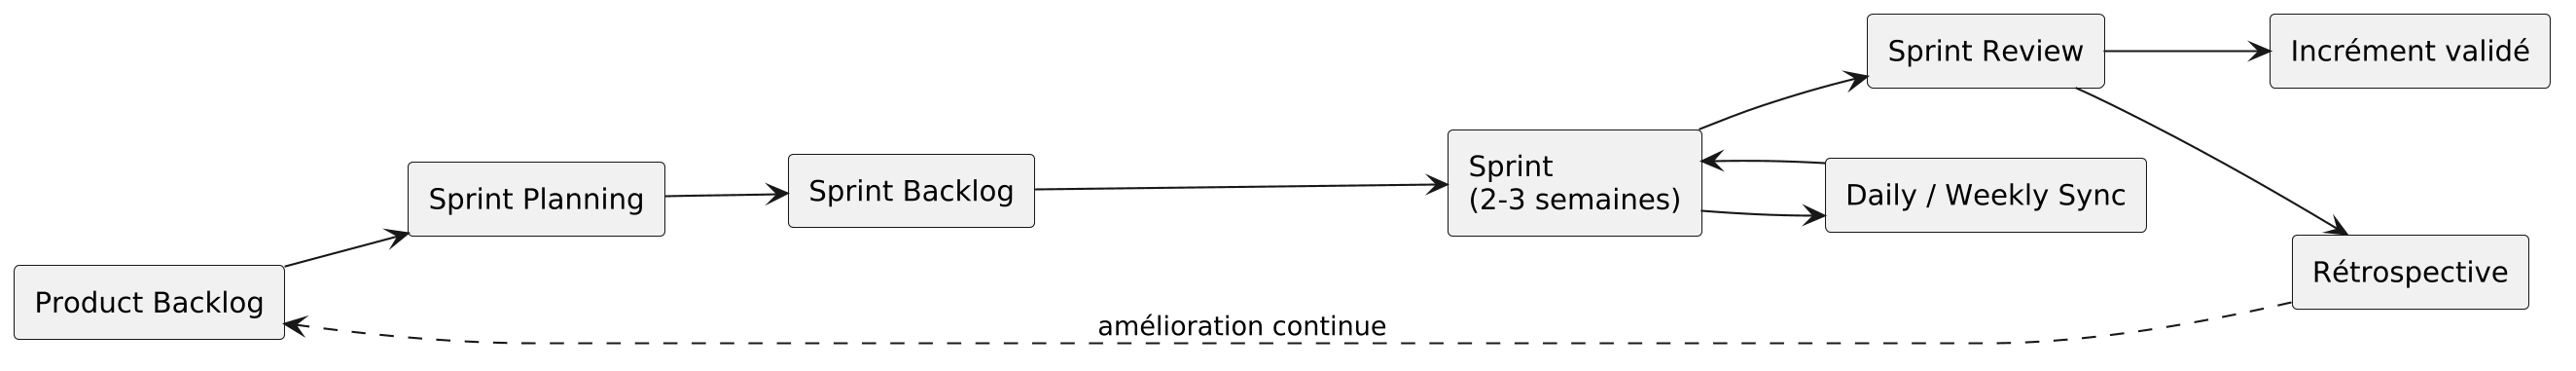
\includegraphics[width=0.88\textwidth,height=0.35\textheight,keepaspectratio]{img/fig_1_1_scrum.png}
    \caption{Processus M\'ethodologique Scrum Appliqu\'e au Projet CyberSec-ASM}
    \label{fig:scrum_process}
\end{figure}

\subsection{Product Backlog Global}
\par Le \textit{Product Backlog} constitue le r\'epertoire central de l'ensemble des exigences fonctionnelles et techniques du projet. Chaque exigence est formul\'ee sous la forme d'une \textit{User Story} (US) selon le formalisme standard : \textit{\og En tant que [Acteur], je veux [Action] afin de [B\'en\'efice] \fg{}}. Le tableau~\ref{tab:product_backlog} pr\'esente la liste ordonnanc\'ee des 30 User Stories prioritaires r\'eparties sur les six sprints.

\begin{table}[H]
\centering
\caption{Product Backlog Global du Projet CyberSec-ASM (30 User Stories)}
\label{tab:product_backlog}
\resizebox{\textwidth}{!}{%
\begin{tabular}{|c|L|L|c|c|c|}
\hline
\textbf{ID} & \textbf{Acteur} & \textbf{User Story (Description)} & \textbf{Priorit\'e} & \textbf{Est. (j)} & \textbf{Sprint} \\
\hline
US01 & Analyste / Admin & S'authentifier de mani\`ere s\'ecuris\'ee avec gestion des sessions JWT & Must Have & 2 & Sprint 1 \\
\hline
US02 & Administrateur & G\'erer les utilisateurs, assigner les r\^oles RBAC et les quotas & Must Have & 3 & Sprint 1 \\
\hline
US03 & Analyste & Cr\'eer un projet d'audit et configurer le p\'erim\`etre des cibles & Must Have & 3 & Sprint 1 \\
\hline
US04 & Analyste & T\'el\'everser et valider le document de preuve d'autorisation (PoA) & Must Have & 2 & Sprint 1 \\
\hline
US05 & Auditeur & V\'erifier la validit\'e juridique et l'historique des mandats PoA & Should Have & 2 & Sprint 1 \\
\hline
US06 & Analyste & Lancer un scan de reconnaissance (Nmap, Nuclei, Gobuster, etc.) & Must Have & 4 & Sprint 2 \\
\hline
US07 & Analyste & Choisir le profil d'intensit\'e de scan (Silent, Balanced, Aggressive) & Must Have & 2 & Sprint 2 \\
\hline
US08 & Analyste & Normaliser automatiquement les sorties brutes en format structur\'e JSON & Must Have & 4 & Sprint 2 \\
\hline
US09 & Analyste & Suivre l'\'etat d'avancement d'un scan en temps r\'eel via Redis Streams & Must Have & 3 & Sprint 2 \\
\hline
US10 & Analyste & Consulter les journaux bruts (\textit{raw logs}) avec citations de lignes & Should Have & 2 & Sprint 2 \\
\hline
US11 & Analyste & Ex\'ecuter des tests d'injection (SQLi, XSS, Command Injection) & Must Have & 4 & Sprint 3 \\
\hline
US12 & Analyste & D\'eployer un conteneur sandbox vuln\'erable isol\'e (DVWA, bWAPP) & Must Have & 4 & Sprint 3 \\
\hline
US13 & Analyste & D\'etruire et r\'einitialiser l'environnement de bac \`a sable & Must Have & 2 & Sprint 3 \\
\hline
US14 & Analyste & Tester la pr\'esence et le comportement d'un WAF externe & Should Have & 3 & Sprint 3 \\
\hline
US15 & Administrateur & Isoler le socket Docker via socket-proxy pour prot\'eger l'h\^ote & Must Have & 2 & Sprint 3 \\
\hline
US16 & Analyste & Solliciter l'IA locale pour analyser les constats de vuln\'erabilit\'e & Must Have & 4 & Sprint 4 \\
\hline
US17 & Analyste & G\'en\'erer des scripts de rem\'ediation durcis (Bash, Ansible, Dockerfile) & Must Have & 4 & Sprint 4 \\
\hline
US18 & Analyste & Valider le respect du sch\'ema Pydantic strict pour \'eviter les hallucinations & Must Have & 3 & Sprint 4 \\
\hline
US19 & Analyste & Appliquer et t\'el\'echarger les correctifs de s\'ecurit\'e propos\'es & Should Have & 2 & Sprint 4 \\
\hline
US20 & Analyste & Consulter la synth\`ese manag\'eriale et l'impact m\'etier g\'en\'er\'es par l'IA & Should Have & 2 & Sprint 4 \\
\hline
US21 & Analyste & Visualiser la topologie des actifs sous forme de graphe relationnel & Must Have & 4 & Sprint 5 \\
\hline
US22 & Analyste & Calculer le rayon d'impact (\textit{blast radius}) par l'algorithme BFS & Must Have & 3 & Sprint 5 \\
\hline
US23 & Analyste & Collecter des renseignements passifs OSINT (DNS, WHOIS, SSL) & Must Have & 3 & Sprint 5 \\
\hline
US24 & Client & Consulter la vue synth\'etique du tableau de bord restreinte \`a son scope & Must Have & 2 & Sprint 5 \\
\hline
US25 & Client / Analyste & Poser des questions de s\'ecurit\'e au Chatbot conversationnel IA & Should Have & 3 & Sprint 5 \\
\hline
US26 & Analyste / Client & G\'en\'erer et exporter les rapports d'expertise (PDF sign\'e, HTML, JSON) & Must Have & 4 & Sprint 6 \\
\hline
US27 & Client & Recevoir et acquitter les alertes de s\'ecurit\'e critiques & Must Have & 2 & Sprint 6 \\
\hline
US28 & Auditeur / Admin & Consulter le journal d'audit immuable (\textit{Audit Logs}) infalsifiable & Must Have & 3 & Sprint 6 \\
\hline
US29 & Auditeur / Admin & Superviser l'\'etat de sant\'e et la disponibilit\'e des microservices & Must Have & 2 & Sprint 6 \\
\hline
US30 & DevSecOps & Ex\'ecuter le pipeline CI/CD automatis\'e avec portes de s\'ecurit\'e & Must Have & 4 & Sprint 6 \\
\hline
\end{tabular}}%
\end{table}

\subsection{Sprint Backlogs D\'etaill\'es}
\par Afin de garantir une ex\'ecution m\'ethodique, les User Stories ont \'et\'e ventil\'ees en six \textit{Sprint Backlogs}. Chaque sprint comporte des objectifs pr\'ecis, des crit\`eres de validation et une charge estim\'ee en jours-homme.

\begin{table}[H]
\centering
\caption{D\'ecomposition D\'etaill\'ee des Sprint Backlogs (Sprints 1 \`a 6)}
\label{tab:sprint_backlogs_detail}
\resizebox{\textwidth}{!}{%
\begin{tabular}{|c|c|L|c|c|L|}
\hline
\textbf{Sprint} & \textbf{US ID} & \textbf{Intitul\'e de la T\^ache / User Story} & \textbf{Priorit\'e} & \textbf{Est. (j)} & \textbf{Crit\`ere d'Acceptation (DoD)} \\
\hline
\multirow{5}{*}{\textbf{Sprint 1}} & US01 & Authentification JWT et contr\^ole des sessions & Must & 2 & Token valide \'emis, expiration contr\^ol\'ee \\
\cline{2-6}
 & US02 & Gestion des r\^oles RBAC (Admin, Analyst, Auditor, Client) & Must & 3 & Middleware de filtrage par r\^ole actif \\
\cline{2-6}
 & US03 & Cr\'eation de projet et saisie du p\'erim\`etre des cibles & Must & 3 & Enregistrement en base PostgreSQL valid\'e \\
\cline{2-6}
 & US04 & T\'el\'eversement et validation du mandat PoA obligatoire & Must & 2 & V\'erification de signature et hachage SHA-256 \\
\cline{2-6}
 & US05 & Contr\^ole juridique des preuves d'autorisation & Should & 2 & Blocage logiciel si PoA absent ou expir\'e \\
\hline
\multirow{5}{*}{\textbf{Sprint 2}} & US06 & Int\'egration du moteur d'orchestration des scanners & Must & 4 & Ex\'ecution asynchrone de Nmap, Nuclei, etc. \\
\cline{2-6}
 & US07 & Gestion des profils de scan et param\'etrage du jitter & Must & 2 & Profils Silent, Balanced, Aggressive op\'erationnels \\
\cline{2-6}
 & US08 & Pipeline de normalisation des r\'esultats \texttt{ResultParser} & Must & 4 & Sorties JSON unifi\'ees avec s\'ev\'erit\'e et CVE \\
\cline{2-6}
 & US09 & T\'el\'em\'etrie temps r\'eel et suivi de progression Redis Streams & Must & 3 & \'Ev\'enements publi\'es et consomm\'es sans perte \\
\cline{2-6}
 & US10 & Visualisation des logs bruts et tra\c{c}abilit\'e des lignes & Should & 2 & Lignes de preuves surlign\'ees dans l'IHM \\
\hline
\multirow{5}{*}{\textbf{Sprint 3}} & US11 & Module d'audit d'injections et vuln\'erabilit\'es applicatives & Must & 4 & D\'etection confirm\'ee de failles OWASP Top 10 \\
\cline{2-6}
 & US12 & D\'eploiement dynamique de conteneurs sandbox isol\'es & Must & 4 & Instanciation DVWA/bWAPP en r\'eseau isol\'e \\
\cline{2-6}
 & US13 & Cycle de vie et destruction automatique des sandboxes & Must & 2 & Nettoyage complet des ressources apr\`es test \\
\cline{2-6}
 & US14 & D\'etection et \'evaluation de contournement WAF & Should & 3 & Rapports d'analyse WAF d\'etaill\'es \\
\cline{2-6}
 & US15 & Durcissement de l'acc\`es Docker via \texttt{socket-proxy} & Must & 2 & Interdiction des privil\`eges root sur l'h\^ote \\
\hline
\multirow{5}{*}{\textbf{Sprint 4}} & US16 & Int\'egration du serveur d'inf\'erence local Ollama & Must & 4 & Mod\`ele \texttt{qwen2.5-coder:7b} op\'erationnel \\
\cline{2-6}
 & US17 & G\'en\'eration automatis\'ee de scripts Remediation-as-Code & Must & 4 & Scripts Bash, Ansible et Dockerfile syntaxiques \\
\cline{2-6}
 & US18 & Validation stricte du format JSON via sch\'ema Pydantic & Must & 3 & 0\% d'hallucination de format en sortie \\
\cline{2-6}
 & US19 & T\'el\'echargement s\'ecuris\'e des correctifs de s\'ecurit\'e & Should & 2 & Fichiers de correction g\'en\'er\'es et sign\'es \\
\cline{2-6}
 & US20 & G\'en\'eration de synth\`eses d'impact pour d\'ecideurs & Should & 2 & R\'esum\'e manag\'erial clair et actionnable \\
\hline
\multirow{5}{*}{\textbf{Sprint 5}} & US21 & Mod\'elisation et affichage du Graphe de Connaissances & Must & 4 & Rendu interactif via Cytoscape.js \\
\cline{2-6}
 & US22 & Impl\'ementation du calcul de Blast Radius (BFS NetworkX) & Must & 3 & Propagation d'impact calcul\'ee en $<75$~ms \\
\cline{2-6}
 & US23 & Renseignement passif OSINT (DNS, WHOIS, Certificats) & Must & 3 & Donn\'ees agr\'eg\'ees sans envoi de paquets actifs \\
\cline{2-6}
 & US24 & Vue IHM restreinte pour le profil Client & Must & 2 & Dashboard filtr\'e sur les actifs autoris\'es \\
\cline{2-6}
 & US25 & Co-pilote conversationnel IA d'assistance & Should & 3 & R\'eponses contextuelles bas\'ees sur l'audit \\
\hline
\multirow{5}{*}{\textbf{Sprint 6}} & US26 & Moteur de g\'en\'eration et export de rapports d'expertise & Must & 4 & Rapports PDF, HTML et JSON t\'el\'echargeables \\
\cline{2-6}
 & US27 & Centre de notification et d'acquittement d'alertes & Must & 2 & Alertes par e-mail et interface web \\
\cline{2-6}
 & US28 & Journalisation immuable d'audit (\textit{Audit Logs}) & Must & 3 & \'Ev\'enements infalsifiables horodat\'es \\
\cline{2-6}
 & US29 & Surveillance de l'\'etat de sant\'e du syst\`eme (\textit{Health}) & Must & 2 & M\'etriques CPU, RAM, conteneurs affich\'ees \\
\cline{2-6}
 & US30 & Int\'egration du pipeline DevSecOps CI/CD sous GitHub & Must & 4 & 8 portes de s\'ecurit\'e bloquantes valid\'ees \\
\hline
\end{tabular}}%
\end{table}

\section*{Conclusion}
\par Ce premier chapitre a permis d'exposer le cadre g\'en\'eral du projet, en d\'emontrant par une analyse comparative approfondie les lacunes des outils existants et l'int\'er\^et d'une approche unifi\'ee semi-agentique. Nous avons d\'efini la probl\'ematique, les objectifs, le p\'erim\`etre et la m\'ethodologie de conduite Agile Scrum. Le chapitre suivant d\'eveloppe l'\'etat de l'art scientifique et l'\'etude comparative des technologies de r\'ef\'erence.

        \clearpage
        
        \chapter{\'Etat de l'Art et \'Etude Comparative}

\section*{Introduction}
\par Ce deuxi\`eme chapitre \'etablit les fondements th\'eoriques, m\'ethodologiques et technologiques n\'ecessaires \`a la conception de notre plateforme. Nous commen\c{c}ons par exposer les principes fondamentaux de la cybers\'ecurit\'e et analysons les dix risques majeurs du r\'ef\'erentiel OWASP Top 10. Nous d\'eveloppons ensuite les concepts cl\'es de la gestion continue de la surface d'attaque (\textit{Attack Surface Management} -- ASM) et pr\'esentons en d\'etail les m\'ecanismes internes des outils de reconnaissance de r\'ef\'erence. Par la suite, nous approfondissons le paradigme DevSecOps, la s\'ecurit\'e de la cha\^ine logicielle, l'apport de l'intelligence artificielle locale contrainte et les architectures microservices \'ev\'enementielles. Enfin, nous menons une \'etude comparative syst\'ematique qui justifie rationnellement chaque choix technologique au regard des exigences du projet.

\section{Fondements de la Cybers\'ecurit\'e}
\subsection{D\'efinition et Enjeux Contemporains}
\par La cybers\'ecurit\'e regroupe l'ensemble des technologies, processus et mesures de contr\^ole con\c{c}us pour prot\'eger les syst\`emes informatiques, les r\'eseaux, les programmes et les donn\'ees contre les cyberattaques. Selon l'Union Internationale des T\'el\'ecommunications (UIT)~\cite{itu}, l'expansion du num\'erique s'accompagne d'une professionnalisation accrue des menaces. Les organisations modernes, dont les activit\'es reposent sur des infrastructures interconnect\'ees et expos\'ees sur Internet, sont r\'eguli\`erement la cible d'attaques visant le vol de propri\'et\'e intellectuelle, l'interruption d'activit\'e ou l'extorsion de fonds. Cybersecurity Ventures~\cite{cyberventures} estime le co\^ut annuel mondial de la cybercriminalit\'e \`a plusieurs milliers de milliards de dollars, soulignant l'obligation pour les entreprises de d\'eployer des approches d'audit continues et proactives.

\subsection{Piliers Fondamentaux de la S\'ecurit\'e}
\par La posture de s\'ecurit\'e d'un syst\`eme d'information repose traditionnellement sur la triade \textbf{CIA} (Confidentialit\'e, Int\'egrit\'e, Disponibilit\'e) et ses principes directeurs associ\'es :
\begin{itemize}
    \item \textbf{Confidentialit\'e :} Garantie que les informations ne sont divulgu\'ees qu'aux personnes, processus ou syst\`emes d\^ument autoris\'es. Sa mise en \oe uvre repose sur des m\'ecanismes de chiffrement fort en transit (TLS 1.3) et au repos (AES-256), associ\'es \`a un contr\^ole d'acc\`es strict.
    \item \textbf{Int\'egrit\'e :} Pr\'eservation de l'exactitude, de la compl\'etude et de la non-alt\'eration des donn\'ees tout au long de leur cycle de vie, garantie par des signatures num\'eriques et des fonctions de hachage cryptographique (SHA-256).
    \item \textbf{Disponibilit\'e :} Maintien de l'accessibilit\'e op\'erationnelle et de la continuit\'e de service pour les utilisateurs l\'egitimes face aux pannes mat\'erielles, aux congestions r\'eseau ou aux attaques volum\'etriques.
    \item \textbf{Authentification et Autorisation :} Processus \`a deux facteurs consistant d'abord \`a prouver formellement l'identit\'e revendiqu\'ee (\textit{Authentification}), puis \`a valider les privil\`eges attribu\'es selon le principe du moindre privil\`ege (\textit{Autorisation}).
    \item \textbf{Tra\c{c}abilit\'e et Non-r\'epudiation :} Capacit\'e d'attribuer sans \'equivoque toute action ou transaction \`a une entit\'e donn\'ee, emp\^echant la contestation ult\'erieure gr\^ace \`a des journaux d'audit immuables et horodat\'es.
\end{itemize}

\section{Le R\'ef\'erentiel OWASP Top 10}
\par L'\textit{Open Worldwide Application Security Project} (OWASP)~\cite{owasp2021} est une autorit\'e de r\'ef\'erence internationale en s\'ecurit\'e applicative. Son classement d\'ecennal \textbf{OWASP Top 10} synth\'etise les risques de s\'ecurit\'e les plus r\'epandus et les plus critiques affectant les architectures web :
\begin{itemize}
    \item \textbf{A01:2021 -- Rupture du Contr\^ole d'Acc\`es (Broken Access Control) :} D\'efaillances dans l'application des restrictions d'acc\`es permettant \`a des utilisateurs non privil\'egi\'es d'acc\'eder \`a des ressources prot\'eg\'ees ou d'alt\'erer des enregistrements appartenant \`a des tiers (failles IDOR, contournement de contr\^ole RBAC).
    \item \textbf{A02:2021 -- D\'efaillances Cryptographiques (Cryptographic Failures) :} Utilisation d'algorithmes obsol\`etes (MD5, SHA1), absence de chiffrement des donn\'ees sensibles ou transmission non s\'ecuris\'ee en clair sur le r\'eseau.
    \item \textbf{A03:2021 -- Injections (Injection) :} D\'efaut de neutralisation des donn\'ees fournies par l'utilisateur, permettant d'ex\'ecuter des instructions arbitraires dans un interpr\'eteur (injections SQL, injections de commandes syst\`eme, Cross-Site Scripting).
    \item \textbf{A04:2021 -- Conception Non S\'ecuris\'ee (Insecure Design) :} Faiblesses architecturales r\'esultant de l'absence de mod\'elisation des menaces et d'application des principes de conception s\'ecuris\'ee d\`es l'amont du projet.
    \item \textbf{A05:2021 -- Mauvaise Configuration de S\'ecurit\'e (Security Misconfiguration) :} Services ou ports superflus activ\'es, messages d'erreur verbeux r\'ev\'elant des traces de pile, identifiants par d\'efaut non modifi\'es ou absence d'en-t\^etes de s\'ecurit\'e (HSTS, CSP).
    \item \textbf{A06:2021 -- Composants Vuln\'erables et Obsol\`etes :} Utilisation de biblioth\`eques, d\'ependances logicielles ou modules tiers contenant des failles document\'ees dans les bases de vuln\'erabilit\'es publiques (CVEs).
    \item \textbf{A07:2021 -- D\'efaillances d'Identification et d'Authentification :} Vuln\'erabilit\'es facilitant le bourrage d'identifiants (\textit{credential stuffing}), l'\'enum\'eration de comptes ou le d\'etournement de session.
    \item \textbf{A08:2021 -- Manque d'Int\'egrit\'e des Donn\'ees et du Logiciel :} Risques li\'es \`a la d\'es\'erialisation d'objets non s\'ecuris\'ee ou \`a l'inclusion de composants logiciels non v\'erifi\'es dans les cha\^ines CI/CD.
    \item \textbf{A09:2021 -- D\'efaillances de Journalisation et de Surveillance :} Absence ou insuffisance de journaux d'audit, retardant la d\'etection des intrusions et rendant impossibles les investigations m\'edico-l\'egales.
    \item \textbf{A10:2021 -- Falsification de Requ\^ete C\^ot\'e Serveur (SSRF) :} Vuln\'erabilit\'e permettant \`a un attaquant d'inciter l'application c\^ot\'e serveur \`a \'emettre une requ\^ete HTTP/TCP vers une ressource interne non expos\'ee.
\end{itemize}

\par La figure~\ref{fig:owasp_heat} positionne ces dix cat\'egories de risques selon leur niveau d'exploitabilit\'e et de d\'etectabilit\'e.

\begin{figure}[H]
\centering
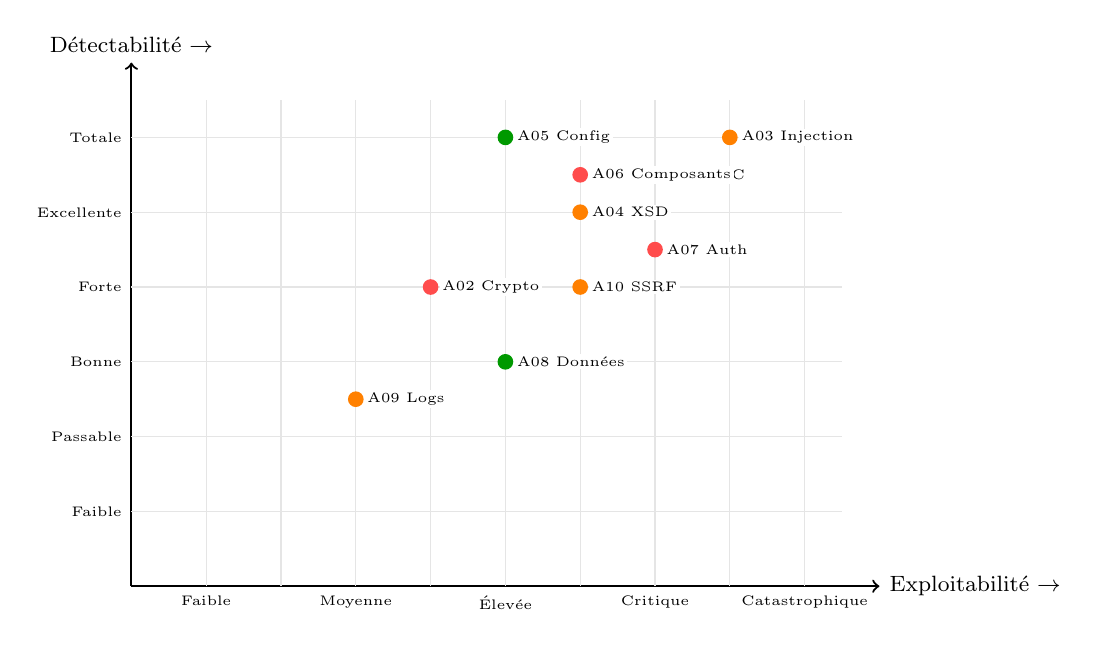
\begin{tikzpicture}[scale=0.95]
\draw[->, thick] (0,0) -- (10,0) node[right, font=\footnotesize]{Exploitabilit\'e $\rightarrow$};
\draw[->, thick] (0,0) -- (0,7) node[above, font=\footnotesize]{D\'etectabilit\'e $\rightarrow$};
\foreach \x in {1,2,3,4,5,6,7,8,9} \draw[gray!20] (\x,0) -- (\x,6.5);
\foreach \y in {1,2,3,4,5,6} \draw[gray!20] (0,\y) -- (9.5,\y);
\foreach \x/\l in {1/Faible,3/Moyenne,5/\'Elev\'ee,7/Critique,9/Catastrophique}
    \node[font=\tiny, below] at (\x,0) {\l};
\foreach \y/\l in {1/Faible,2/Passable,3/Bonne,4/Forte,5/Excellente,6/Totale}
    \node[font=\tiny, left] at (0,\y) {\l};
\node[circle, fill=red!70, inner sep=2pt, label={[font=\tiny, fill=white, inner sep=1pt]right:A01 BAC}] at (7,5.5) {};
\node[circle, fill=red!70, inner sep=2pt, label={[font=\tiny, fill=white, inner sep=1pt]right:A02 Crypto}] at (4,4) {};
\node[circle, fill=orange, inner sep=2pt, label={[font=\tiny, fill=white, inner sep=1pt]right:A03 Injection}] at (8,6) {};
\node[circle, fill=orange, inner sep=2pt, label={[font=\tiny, fill=white, inner sep=1pt]right:A04 XSD}] at (6,5) {};
\node[circle, fill=green!60!black, inner sep=2pt, label={[font=\tiny, fill=white, inner sep=1pt]right:A05 Config}] at (5,6) {};
\node[circle, fill=red!70, inner sep=2pt, label={[font=\tiny, fill=white, inner sep=1pt]right:A06 Composants}] at (6,5.5) {};
\node[circle, fill=red!70, inner sep=2pt, label={[font=\tiny, fill=white, inner sep=1pt]right:A07 Auth}] at (7,4.5) {};
\node[circle, fill=green!60!black, inner sep=2pt, label={[font=\tiny, fill=white, inner sep=1pt]right:A08 Donn\'ees}] at (5,3) {};
\node[circle, fill=orange, inner sep=2pt, label={[font=\tiny, fill=white, inner sep=1pt]right:A09 Logs}] at (3,2.5) {};
\node[circle, fill=orange, inner sep=2pt, label={[font=\tiny, fill=white, inner sep=1pt]right:A10 SSRF}] at (6,4) {};
\end{tikzpicture}
\caption{Matrice des Risques OWASP Top 10 (2021) -- Exploitabilit\'e vs D\'etectabilit\'e}
\label{fig:owasp_heat}
\end{figure}

\section{Gestion Continue de la Surface d'Attaque (ASM)}
\subsection{D\'efinition et Principes}
\par La surface d'attaque d'une organisation repr\'esente l'ensemble cumul\'e des points d'entr\'ee et vecteurs d'exposition par lesquels un attaquant potentiel peut tenter d'infiltrer un r\'eseau, de corrompre un syst\`eme ou d'exfiltrer des donn\'ees. L'\textit{Attack Surface Management} (ASM) est la discipline d'ing\'enierie consistant \`a identifier, cartographier, analyser et r\'eduire en continu cette surface d'exposition num\'erique externe.

\subsection{Cycle de Vie du Processus ASM}
\par Une d\'emarche ASM mature s'organise selon un cycle it\'eratif structur\'e en six phases interd\'ependantes, illustr\'e sur la figure~\ref{fig:asm_flow} :
\begin{enumerate}
    \item \textbf{D\'ecouverte (Discovery) :} Recherche et d\'etection exhaustive de tous les actifs expos\'es sur Internet associ\'es \`a l'organisation (domaines, sous-domaines, plages IP, services Cloud, certificats).
    \item \textbf{Inventaire (Inventory) :} Structuration et centralisation des donn\'ees d'actifs au sein d'un r\'ef\'erentiel d'inventaire unifi\'e.
    \item \textbf{Classification (Classification) :} \'Evaluation de la nature des actifs, de leur niveau d'exposition et de leur criticit\'e m\'etier.
    \item \textbf{Audit et Analyse (Assessment) :} Ex\'ecution de scans techniques cibl\'es pour d\'etecter les vuln\'erabilit\'es, faiblesses applicatives et d\'efauts de configuration.
    \item \textbf{Priorisation (Prioritization) :} \'Evaluation du rayon d'impact (\textit{blast radius}) et corr\'elation relationnelle pour hi\'erarchiser les alertes en fonction de la menace r\'eelle.
    \item \textbf{Rem\'ediation (Remediation) :} D\'eploiement de correctifs logiciels, durcissement des r\`egles de filtrage et validation post-rem\'ediation.
\end{enumerate}

\begin{figure}[H]
    \centering
    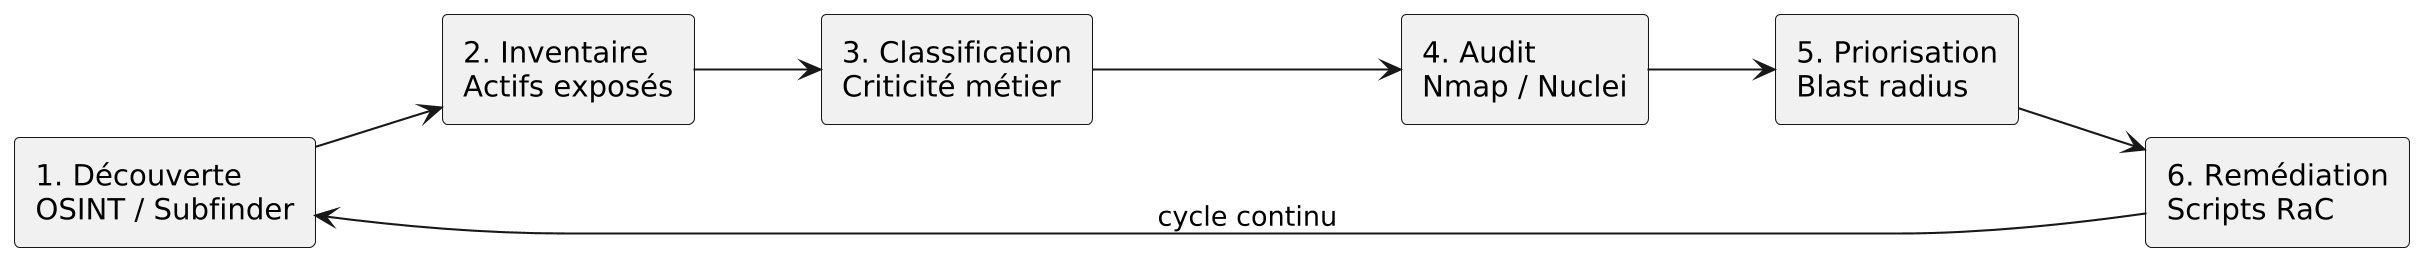
\includegraphics[width=0.95\textwidth]{img/fig_2_2_asm.png}
    \caption{Cycle de Vie du Processus d'Attack Surface Management (ASM)}
    \label{fig:asm_flow}
\end{figure}

\section{Reconnaissance et Outils d'Audit de S\'ecurit\'e}
\subsection{R\^ole et Typologie de la Reconnaissance}
\par La reconnaissance constitue la premi\`ere phase incontournable de tout audit technique de s\'ecurit\'e. Elle se d\'ecompose en deux grandes modalit\'es :
\begin{itemize}
    \item \textbf{Reconnaissance Passive (OSINT) :} Collecte d'informations sans interaction r\'eseau directe avec l'infrastructure de la cible (interrogation des registres WHOIS, des serveurs DNS publics, des registres de transparence de certificats \texttt{crt.sh}). Elle garantit une discr\'etion op\'erationnelle totale.
    \item \textbf{Reconnaissance Active :} \'Emission de paquets r\'eseau et de requ\^etes applicatives directement vers les h\^otes cibles (balayage de ports SYN, requ\^etes HTTP/HTTPS, \'enum\'eration de r\'epertoires). Elle fournit une cartographie technique exacte des services et versions expos\'es.
\end{itemize}

\subsection{Outils d'Audit Int\'egr\'es dans la Plateforme}
\par Notre plateforme int\`egre cinq outils de reconnaissance et d'audit de s\'ecurit\'e de r\'ef\'erence, encapsul\'es au sein de conteneurs isol\'es :

\begin{itemize}
    \item \textbf{\color{blue!80!black}[\,Nmap\,] -- Network Mapper~\cite{nmap} :} Outil d'exploration r\'eseau mondialement reconnu. Il utilise l'\'emission de paquets TCP SYN bruts (\textit{SYN stealth scan}) pour d\'eterminer l'\'etat des ports, identifie les banni\`eres applicatives et d\'etecte les syst\`emes d'exploitation via l'analyse de signatures TCP/IP. Son moteur NSE (\textit{Nmap Scripting Engine}) permet d'ex\'ecuter des scripts Lua pour \'evaluer des vuln\'erabilit\'es connues.
    \item \textbf{\color{purple!80!black}[\,Nuclei\,] -- Vulnerability Scanner~\cite{nuclei} :} Moteur d'\'evaluation de vuln\'erabilit\'es pilot\'e par des mod\`eles d\'eclaratifs YAML communautaires. Con\c{c}u en langage Go, il excelle dans la d\'etection rapide de failles web complexes (CVEs r\'ecentes, faiblesses d'authentification, fuites de donn\'ees d'infrastructure) en envoyant des requ\^etes cibl\'ees avec un taux de faux positifs inf\'erieur aux scanners g\'en\'eriques.
    \item \textbf{\color{cyan!80!black}[\,Gobuster\,] -- Content \& DNS Enumeration~\cite{gobuster} :} Outil d'\'enum\'eration brute rapide d\'evelopp\'e en Go exploitant des routines concurrentes. Il permet d'identifier les chemins, r\'epertoires cach\'es, fichiers sensibles d'environnement (\texttt{.env}, \texttt{.git}, sauvegardes \texttt{.bak}) et sous-domaines par confrontation \`a des dictionnaires volumineux (\textit{SecLists}).
    \item \textbf{\color{green!60!black}[\,Subfinder\,] -- Passive OSINT Subdomains~\cite{subfinder} :} Outil d'\'enum\'eration passive de sous-domaines. Il agr\`ege les donn\'ees issues de dizaines de sources passives ouvertes sans jamais contacter directement la cible, assurant la d\'ecouverte exhaustive des p\'erim\`etres oubli\'es.
    \item \textbf{\color{orange!80!black}[\,WPScan\,] -- WordPress Vulnerability Scanner~\cite{wpscan} :} Scanner sp\'ecialis\'e dans l'audit des syst\`emes WordPress. Il analyse le code source HTML, les en-t\^etes HTTP et les r\'epertoires standards pour recenser les th\`emes et extensions obsol\`etes r\'epertori\'es dans la base de donn\'ees WPScan Vulnerability Database.
\end{itemize}

\section{DevSecOps et S\'ecurit\'e de la Cha\^ine Logicielle}
\subsection{Origine et Philosophie Shift-Left}
\par Le mod\`ele traditionnel de d\'eveloppement logiciel r\'eservait les contr\^oles de s\'ecurit\'e \`a la fin du cycle de livraison, juste avant le passage en production. Cette approche tardive engendrait des goulots d'\'etranglement op\'erationnels majeurs : la correction d'une faille architecturale ou d'une d\'ependance vuln\'erable d\'ecouverte tardivement entra\^inant des co\^uts prohibitifs et des retards de d\'eploiement importants.
\par Le paradigme \textbf{DevSecOps}~\cite{devsecops} propose de fusionner le d\'eveloppement (\textit{Dev}), la s\'ecurit\'e (\textit{Sec}) et les op\'erations (\textit{Ops}) en int\'egrant des contr\^oles automatis\'es \`a chaque \'etape du cycle de vie logiciel, comme l'illustre la figure~\ref{fig:devsecops_cycle}. Cette philosophie, qualifi\'ee de \textbf{\textit{Shift-Left Security}}, consiste \`a d\'eplacer les v\'erifications de s\'ecurit\'e le plus t\^ot possible dans la cha\^ine de fabrication logicielle, permettant aux d\'eveloppeurs d'identifier et de corriger les vuln\'erabilit\'es d\`es la phase d'\'ecriture du code source.

\begin{figure}[H]
\centering
\begin{tikzpicture}[
    node distance=5mm and 6mm,
    stage/.style={draw, rounded corners=3pt, fill=blue!8, draw=blue!50, thick, minimum width=24mm, minimum height=10mm, align=center, font=\tiny\bfseries},
    secgate/.style={draw, rounded corners=3pt, fill=red!10, draw=red!60, thick, minimum width=24mm, minimum height=8mm, align=center, font=\tiny},
    arrow/.style={-{Stealth[length=2mm]}, thick, draw=blue!70}
]
\node[stage] (plan) {1. Planifier\\\& Coder};
\node[stage, right=of plan] (build) {2. Construire\\\& Tester};
\node[stage, right=of build] (scan) {3. Scanner\\\& Valider};
\node[stage, right=of scan] (sign) {4. Signer\\\& Publier};
\node[stage, right=of sign] (deploy) {5. D\'eployer\\en Prod};

\node[secgate, below=4mm of plan] (g1) {IDE Linting\\Pre-commit};
\node[secgate, below=4mm of build] (g2) {SAST (Psalm/Bandit)\\SCA D\'ependances};
\node[secgate, below=4mm of scan] (g3) {SBOM (Syft)\\Trivy Container};
\node[secgate, below=4mm of sign] (g4) {Cosign Signature\\Attestation OCI};
\node[secgate, below=4mm of deploy] (g5) {UFW + Nginx TLS\\Audit Logs};

\draw[arrow] (plan) -- (build);
\draw[arrow] (build) -- (scan);
\draw[arrow] (scan) -- (sign);
\draw[arrow] (sign) -- (deploy);

\draw[dashed, ->, draw=red!70] (g1) -- (plan);
\draw[dashed, ->, draw=red!70] (g2) -- (build);
\draw[dashed, ->, draw=red!70] (g3) -- (scan);
\draw[dashed, ->, draw=red!70] (g4) -- (sign);
\draw[dashed, ->, draw=red!70] (g5) -- (deploy);
\end{tikzpicture}
\caption{Cycle de Livraison DevSecOps : Int\'egration Continue des Portes de S\'ecurit\'e (Shift-Left)}
\label{fig:devsecops_cycle}
\end{figure}

\subsection{S\'ecurit\'e de la Cha\^ine d'Approvisionnement Logicielle (Software Supply Chain)}
\par Dans les applications modernes, plus de 80\,\% du code d\'eploy\'e provient de d\'ependances open-source et de conteneurs tiers. Les attaquants ciblent d\'esormais fr\'equemment la cha\^ine d'approvisionnement logicielle (\textit{Supply Chain Attacks}) en injectant du code malveillant dans des biblioth\`eques populaires. Pour r\'epondre \`a ce risque, le cadre DevSecOps d\'eploie cinq m\'ecanismes de d\'efense compl\'ementaires :
\begin{itemize}
    \item \textbf{SAST (Static Application Security Testing) :} Analyse statique automatis\'ee du code source au repos sans l'ex\'ecuter. Elle r\'ev\`ele les failles d'impl\'ementation (injections, d\'er\'ef\'erencements de pointeurs nuls, gestion de secrets en clair). Dans notre environnement, \textbf{Psalm}~\cite{psalm} analyse le code PHP/Laravel et \textbf{Bandit}~\cite{bandit} audite le code Python/Flask.
    \item \textbf{SCA (Software Composition Analysis) :} Analyse de la composition logicielle identifiant les d\'ependances tierces obsol\`etes ou affect\'ees par des CVEs connues r\'epertori\'ees dans la base NVD.
    \item \textbf{SBOM (Software Bill of Materials) :} Inventaire exhaustif, standardis\'e et lisible par machine de l'ensemble des composants logiciels, versions et licences int\'egr\'es \`a l'artefact de livraison. Nous exploitons l'outil \textbf{Syft}~\cite{syft} pour g\'en\'erer des fichiers SBOM au standard ouvert \textbf{CycloneDX}.
    \item \textbf{Scan d'Images de Conteneurs :} Analyse multicouche des images Docker permettant d'identifier les vuln\'erabilit\'es pr\'esentes dans le syst\`eme d'exploitation sous-jacent et les packages syst\`eme via l'analyseur de r\'ef\'erence \textbf{Trivy}~\cite{trivy}.
    \item \textbf{Signature Cryptographique de Conteneurs :} Application d'une signature num\'erique immuable sur les images conteneuris\'ees valid\'ees gr\^ace \`a \textbf{Cosign (Sigstore)}~\cite{cosign}. Seules les images d\^ument sign\'ees et v\'erifi\'ees sont autoris\'ees \`a \^etre d\'eploy\'ees sur le serveur de production.
\end{itemize}

\section{Intelligence Artificielle Locale et Grands Mod\`eles de Langage (LLM)}
\subsection{Apport des LLM dans l'Audit de S\'ecurit\'e}
\par L'int\'egration des grands mod\`eles de langage (\textit{Large Language Models} -- LLM) dans les plateformes de s\'ecurit\'e apporte une valeur ajout\'ee d\'ecisive : capacit\'e de synth\'etiser des volumes massifs de journaux techniques pour les d\'ecideurs manag\'eriaux, explication vulgaris\'ee du m\'ecanisme des failles d\'etect\'ees, et g\'en\'eration automatis\'ee de scripts durcis de rem\'ediation (\textit{Remediation-as-Code}).

\subsection{Imp\'eratif de Confidentialit\'e et Mod\`eles Contraints}
\par Le recours \`a des API d'IA h\'eberg\'ees dans le Cloud public (telles qu'OpenAI ou Anthropic) soul\`eve des probl\`emes majeurs de confidentialit\'e industrielle : les vuln\'erabilit\'es critiques d'infrastructures sensibles et les adresses IP d'actifs audit\'es seraient transmises \`a des serveurs tiers.
\par Pour r\'esoudre ce d\'efi, nous avons fait le choix strat\'egique d'un moteur d'inf\'erence local (\textbf{Ollama}) h\'ebergeant le mod\`ele \textbf{\texttt{qwen2.5-coder}}. Cette approche contribue \`a pr\'eserver la confidentialit\'e des donn\'ees en \'evitant leur transmission \`a un fournisseur externe de LLM. De plus, le microservice contribue \`a r\'eduire le risque d'hallucination inh\'erent aux mod\`eles g\'en\'eratifs en imposant un gabarit de prompt syst\`eme (\textit{system prompt}) contraignant la sortie \`a un format JSON strict et exigeant des r\'ef\'erences explicites aux num\'eros de lignes des journaux bruts d'audit (figure~\ref{fig:ai_pipeline}).

\begin{figure}[H]
\centering
\resizebox{0.97\textwidth}{!}{%
\begin{tikzpicture}[
    node distance=5mm and 7mm,
    ibox/.style={draw, rounded corners=3pt, fill=purple!8, draw=purple!50, thick, minimum width=28mm, minimum height=9mm, align=center, font=\tiny},
    arrow/.style={-{Stealth[length=2mm]}, thick, draw=purple!70}
]
\node[ibox] (in) {1. Constat Brut\\+ Contexte Faille};
\node[ibox, right=of in] (prompt) {2. Prompt Contraint\\(R\`egles \& Guardrails)};
\node[ibox, right=of prompt] (llm) {3. LLM Local\\(Ollama / Qwen2.5)};
\node[ibox, right=of llm] (val) {4. Validation Pydantic\\+ V\'erif. Citations};
\node[ibox, right=of val] (out) {5. Remediation-as-Code\\(Bash / Ansible / Docker)};

\draw[arrow] (in) -- (prompt);
\draw[arrow] (prompt) -- (llm);
\draw[arrow] (llm) -- (val);
\draw[arrow] (val) -- (out);
\draw[dashed, ->, draw=red!60] (val.south) .. controls +(0,-6mm) and +(0,-6mm) .. (prompt.south) node[midway, below, font=\tiny]{Rejet \& Fallback si JSON invalide};
\end{tikzpicture}}
\caption{Pipeline de l'IA Locale Contrainte pour la Production de Remediation-as-Code}
\label{fig:ai_pipeline}
\end{figure}

\section{Architectures Microservices et Syst\`emes \'Ev\'enementiels}
\par L'architecture microservices d\'ecompose une application complexe en un ensemble de services autonomes, ind\'ependamment d\'eployables et hautement sp\'ecialis\'es, communiquant via des protocoles r\'eseau l\'egers.
\par Pour une plateforme d'audit o\`u les t\^aches de balayage (scans Nmap, Gobuster) peuvent durer de plusieurs secondes \`a plusieurs dizaines de minutes, une architecture purement synchrone HTTP conduirait in\'evitablement \`a des blocages de requ\^etes (\textit{timeouts}). L'adoption d'un mod\`ele asynchrone pilot\'e par \'ev\'enements via \textbf{Redis Streams} permet de d\'ecoupler le portail web de l'ex\'ecution des scanners (figure~\ref{fig:microservices_pattern}) : les requ\^etes d'audit sont ins\'er\'ees dans un flux persistant, puis consomm\'ees par des processus d\'edi\'es (\textit{workers}) capables de g\'erer les r\'eessais automatiques avec repli exponentiel.

\begin{figure}[H]
\centering
\begin{tikzpicture}[
    node distance=6mm and 8mm,
    cbox/.style={draw, rounded corners=3pt, fill=blue!10, draw=blue!60, thick, minimum width=32mm, minimum height=9mm, align=center, font=\scriptsize\bfseries},
    mbox/.style={draw, rounded corners=3pt, fill=green!10, draw=green!60!black, thick, minimum width=28mm, minimum height=8mm, align=center, font=\tiny},
    rbox/.style={draw, rounded corners=3pt, fill=orange!10, draw=orange!60, thick, minimum width=30mm, minimum height=8mm, align=center, font=\tiny\bfseries},
    arrow/.style={-{Stealth[length=2mm]}, thick}
]
\node[cbox] (client) {Utilisateur / SOC};
\node[cbox, right=14mm of client] (backend) {Back-end Laravel 11\\(Portail + API)};
\node[rbox, below=10mm of backend] (redis) {Redis Streams 7\\(Message Broker)};
\node[mbox, below=10mm of redis] (worker) {Worker Asynchrone\\(Consommation XREADGROUP)};
\node[mbox, left=10mm of worker] (recon) {Microservice Recon\\(Nmap, Nuclei, Gobuster)};
\node[mbox, right=10mm of worker] (ai) {Microservice IA\\(Ollama LLM)};

\draw[arrow, draw=blue!70] (client) -- (backend) node[midway, above, font=\tiny]{HTTPS};
\draw[arrow, draw=orange!70] (backend) -- (redis) node[midway, right, font=\tiny]{XADD scan:requests};
\draw[arrow, draw=orange!70] (redis) -- (worker) node[midway, right, font=\tiny]{\'Ev\'enement de Scan};
\draw[arrow, draw=green!60!black] (worker) -- (recon) node[midway, above, font=\tiny]{REST POST};
\draw[arrow, draw=green!60!black] (worker) -- (ai) node[midway, above, font=\tiny]{REST POST};
\end{tikzpicture}
\caption{Patron d'Architecture Microservices et D\'ecouplage Asynchrone via Redis Streams}
\label{fig:microservices_pattern}
\end{figure}

\section{\'Etude Comparative et Justification des Choix Technologiques}
\par Afin de garantir la robustesse et la p\'erennit\'e du syst\`eme, nous avons men\'e des \'etudes comparatives syst\'ematiques sur chaque brique technologique.

\subsection{Comparatif des Frameworks Backend Web}
\par Le tableau~\ref{tab:comp_backend} synth\'etise l'analyse comparative des principaux frameworks web du march\'e.

\begin{table}[H]
\centering
\caption{Analyse Comparative des Frameworks Web Backend}
\label{tab:comp_backend}
\resizebox{\textwidth}{!}{%
\begin{tabular}{|L|L|L|L|L|}
\hline
\textbf{Crit\`ere} & \textbf{Laravel 11 (PHP)} & \textbf{Django 5 (Python)} & \textbf{Spring Boot (Java)} & \textbf{Express.js (Node)} \\
\hline
ORM \& Mod\'elisation & Eloquent (tr\`es intuitif) & Django ORM (puissant) & Hibernate / JPA (complexe) & Prisma / TypeORM \\
\hline
Syst\`eme de Files / Queues & Natif (Redis, DB) & Celery (externe) & Spring JMS / RabbitMQ & BullMQ (externe) \\
\hline
Authentification \& RBAC & Sanctum + Spatie Permission & Int\'egr\'e & Spring Security (lourd) & Passport.js (manuel) \\
\hline
Moteur de Templates & Blade (performant) & Django Templates & Thymeleaf & EJS / Pug \\
\hline
Courbe d'apprentissage & Mod\'er\'ee & Mod\'er\'ee & \'Elev\'ee & Faible \\
\hline
Expertise Organisme & \'Elev\'ee (Designet Web) & Mod\'er\'ee & Faible & Mod\'er\'ee \\
\hline
\rowcolor{green!15} \textbf{Retenu} & \textbf{Oui} & Non & Non & Non \\
\hline
\end{tabular}}%
\end{table}
\par \textbf{Justification du Choix de Laravel 11 :} Laravel 11 a \'et\'e retenu car il offre une gestion native et \'eprouv\'ee de l'authentification et du contr\^ole d'acc\`es RBAC via Spatie Permission, un ORM Eloquent permettant de manipuler de fa\c{c}on expressive les 14 entit\'es m\'etier du mod\`ele (25 tables physiques au total), et une int\'egration directe des files de messages Redis. Enfin, ce choix capitalise sur l'expertise forte de Designet Web Agency, garantissant la maintenabilit\'e \`a long terme.

\subsection{Comparatif des Frameworks de Microservices Python}
\par Le tableau~\ref{tab:comp_micro} d\'etaille l'\'etude comparative des frameworks l\'egers pour le d\'eveloppement des microservices.

\begin{table}[H]
\centering
\caption{Analyse Comparative des Frameworks de Microservices}
\label{tab:comp_micro}
\resizebox{\textwidth}{!}{%
\begin{tabular}{|L|L|L|L|L|}
\hline
\textbf{Crit\`ere} & \textbf{Flask} & \textbf{FastAPI} & \textbf{Django REST} & \textbf{Nameko} \\
\hline
Empreinte m\'emoire & Tr\`es l\'eg\`ere ($\sim$100 Mo) & L\'eg\`ere ($\sim$120 Mo) & Lourde ($\sim$300 Mo) & Mod\'er\'ee ($\sim$200 Mo) \\
\hline
Gestion des subprocess & Contr\^ole total synchrone & Async / Subprocess & Bloquant & Bas\'ee sur workers \\
\hline
Int\'egration outils CLI & Directe et robuste & Tr\`es bonne & Mod\'er\'ee & Mod\'er\'ee \\
\hline
Courbe d'apprentissage & Tr\`es faible & Mod\'er\'ee & \'Elev\'ee & \'Elev\'ee \\
\hline
\rowcolor{green!15} \textbf{Retenu} & \textbf{Oui} & Non & Non & Non \\
\hline
\end{tabular}}%
\end{table}
\par \textbf{Justification du Choix de Flask :} Flask a \'et\'e s\'electionn\'e pour sa l\'eg\`eret\'e, sa stabilit\'e et son contr\^ole absolu sur les processus syst\`eme (\texttt{subprocess.Popen}) encapsulant Nmap, Nuclei et Gobuster. L'ex\'ecution d'outils CLI lourds s'accommode id\'ealement du mod\`ele synchrone ma\^itris\'e de Flask au sein de conteneurs d\'edi\'es.

\subsection{Comparatif des Moteurs d'IA Locale (LLM)}
\par Le tableau~\ref{tab:comp_ai} pr\'esente la comparaison des moteurs d'inf\'erence locale h\'ebergeant des mod\`eles de langage.

\begin{table}[H]
\centering
\caption{Analyse Comparative des Moteurs d'IA Locale}
\label{tab:comp_ai}
\resizebox{\textwidth}{!}{%
\begin{tabular}{|L|L|L|L|L|}
\hline
\textbf{Crit\`ere} & \textbf{Ollama} & \textbf{LM Studio} & \textbf{LocalAI} & \textbf{vLLM} \\
\hline
Licence Open Source & Oui (MIT) & Propri\'etaire & Oui (MIT) & Oui (Apache 2.0) \\
\hline
Int\'egration Docker & Image officielle durcie & Application bureau & Image officielle & Complexe (CUDA) \\
\hline
Mode Serveur Headless & Natif (API REST :11434) & Limit\'e & Natif & Natif \\
\hline
Gestion des mod\`eles & Int\'egr\'ee (\texttt{pull}, \texttt{run}) & Manuelle & Manuelle & Manuelle \\
\hline
\rowcolor{green!15} \textbf{Retenu} & \textbf{Oui} & Non & Non & Non \\
\hline
\end{tabular}}%
\end{table}
\par \textbf{Justification du Choix d'Ollama et de Qwen2.5-Coder :} Ollama s'int\`egre parfaitement dans un environnement Docker Compose en mode conteneuris\'e sans interface graphique. Le mod\`ele \texttt{qwen2.5-coder} offre un ratio performances/taille optimal pour la production de code syst\`eme (Bash, Ansible, Dockerfile) et respecte fid\`element les structures JSON impos\'ees.

\subsection{Comparatif de la Base de Donn\'ees et du Moteur de Graphe}
\par Le tableau~\ref{tab:comp_db} compare les architectures de persistance de donn\'ees et de mod\'elisation de graphe.

\begin{table}[H]
\centering
\caption{Analyse Comparative des Solutions de Base de Donn\'ees et Graphes}
\label{tab:comp_db}
\resizebox{\textwidth}{!}{%
\begin{tabular}{|L|L|L|L|}
\hline
\textbf{Crit\`ere} & \textbf{PostgreSQL 16 + Apache AGE} & \textbf{MySQL + Neo4j} & \textbf{MongoDB} \\
\hline
Architecture & Instance unifi\'ee (Relationnel + Graphe) & 2 serveurs distincts & Base documentaire seule \\
\hline
Langage Graphe & openCypher natif & Cypher (Neo4j) & Agr\'egations complexes \\
\hline
Support JSONB & Excellent (Index GIN) & Mod\'er\'e & Natif \\
\hline
Empreinte m\'emoire & R\'eduite (une seule instance DB) & \'Elev\'ee (JVM Neo4j + MySQL) & Mod\'er\'ee \\
\hline
\rowcolor{green!15} \textbf{Retenu} & \textbf{Oui} & Non & Non \\
\hline
\end{tabular}}%
\end{table}
\par \textbf{Justification du Choix de PostgreSQL 16 avec Apache AGE :} L'extension Apache AGE permet de manipuler des requ\^etes relationnelles SQL et des graphes openCypher au sein d'une seule et m\^eme instance PostgreSQL. Cette architecture \'evite la redondance et la surcharge m\'emoire li\'ees au d\'eploiement d'un moteur de graphe d\'edi\'e sous JVM (comme Neo4j).

\subsection{Comparatif du Message Broker pour Traitement Asynchrone}
\par Le tableau~\ref{tab:comp_broker} pr\'esente le comparatif des solutions de messagerie et de files d'attente asynchrones.

\begin{table}[H]
\centering
\caption{Analyse Comparative des Syst\`emes de Message Broker}
\label{tab:comp_broker}
\resizebox{\textwidth}{!}{%
\begin{tabular}{|L|L|L|L|}
\hline
\textbf{Crit\`ere} & \textbf{Redis 7 (Streams)} & \textbf{RabbitMQ} & \textbf{Apache Kafka} \\
\hline
Persistance & Oui (AOF / RDB) & Oui & Oui (Partitionn\'ee) \\
\hline
Groupes de Consommateurs & Natif (\texttt{XREADGROUP}) & Natif & Natif \\
\hline
Empreinte m\'emoire & Tr\`es faible ($<$50 Mo) & Mod\'er\'ee ($\sim$150 Mo) & Tr\`es lourde (JVM + Zookeeper/Kraft) \\
\hline
Usage multifonction & Broker + Cache + Sessions & Broker uniquement & Streaming uniquement \\
\hline
\rowcolor{green!15} \textbf{Retenu} & \textbf{Oui} & Non & Non \\
\hline
\end{tabular}}%
\end{table}
\par \textbf{Justification du Choix de Redis 7 Streams :} Redis 7 offre \`a la fois un r\^ole de Message Broker avec persistance et acquittement (\texttt{XACK}), de cache de requ\^etes IHM et de gestionnaire de sessions, r\'eduisant ainsi le nombre de composants d'infrastructure requis.

\subsection{Synth\`ese Globale des Choix Technologiques}
\par Le tableau~\ref{tab:tech_summary} r\'ecapitule l'ensemble des choix technologiques adopt\'es pour la r\'ealisation de la plateforme avec leur justification strat\'egique.

\begin{table}[H]
\centering
\caption{Tableau R\'ecapitulatif de la Pile Technologique Retenue}
\label{tab:tech_summary}
\resizebox{\textwidth}{!}{%
\begin{tabular}{|L|L|L|}
\hline
\textbf{Composant / Couche} & \textbf{Technologie Retenue} & \textbf{Justification Strat\'egique} \\
\hline
Portail Web Backend & Laravel 11 (PHP 8.3) & ORM Eloquent expressif, RBAC Spatie, queues Redis natives. \\
\hline
Microservices d'Audit & Flask 3.1 (Python 3.12) & Empreinte m\'emoire tr\`es l\'eg\`ere, conteneurisation isol\'ee, contr\^ole absolu sur les sous-processus CLI. \\
\hline
Base de Donn\'ees & PostgreSQL 16 + Apache AGE & Instance unifi\'ee supportant \`a la fois SQL relationnel et graphe openCypher. \\
\hline
Message Broker \& Cache & Redis 7 (Streams) & Files persistantes asynchrones, reprise sur panne et cache performant. \\
\hline
Calcul de Rayon d'Impact & NetworkX 3.2 & Algorithmes de parcours en largeur (BFS) ultra-rapides en m\'emoire ($<$75 ms). \\
\hline
IA Locale \& Remediation & Ollama / \texttt{qwen2.5-coder} & Confidentialit\'e totale 100\,\% locale, mod\`ele sp\'ecialiste code, sch\'emas JSON stricts. \\
\hline
Front-end \& Rendu IHM & Blade + Tailwind CSS + Cytoscape.js & Rendu serveur r\'eactif, visualisation dynamique et interactive du graphe. \\
\hline
Conteneurisation \& Proxy & Docker + Docker Socket Proxy & Isolation herm\'etique des conteneurs non-root et filtrage de l'API Docker. \\
\hline
Pipeline DevSecOps & GitHub Actions, Psalm, Bandit, Trivy, Cosign & Automatisation des portes bloquantes (SAST, SCA, SBOM CycloneDX, signature). \\
\hline
\end{tabular}}%
\end{table}

\section*{Conclusion}
\par Ce chapitre a \'etabli l'\'etat de l'art scientifique et conceptuel de la cybers\'ecurit\'e, de l'ASM, des scanners d'audit, du DevSecOps, de l'IA locale et des microservices. Les \'etudes comparatives syst\'ematiques ont justifi\'e l'ensemble des choix technologiques retenus. Le chapitre suivant d\'etaillera l'analyse approfondie des besoins, la mod\'elisation formelle des menaces STRIDE et la conception architecturale de la plateforme.

        \clearpage
        
        \chapter{Analyse des Besoins et Conception du Syst\`eme}

\section*{Introduction}
\par Ce troisi\`eme chapitre pr\'esente la d\'emarche rigoureuse d'analyse des exigences et de conception architecturale de notre plateforme. Nous d\'ebutons par l'analyse exhaustive des besoins fonctionnels, non fonctionnels, des contraintes de s\'ecurit\'e et des exigences l\'egales (PoA). Nous formalisons ensuite la mod\'elisation fonctionnelle \`a travers les diagrammes de cas d'utilisation UML. Par la suite, nous d\'etaillons l'architecture globale en distinguant explicitement les \textbf{7 composants applicatifs m\'etier} et les \textbf{12 conteneurs Docker d'infrastructure}. Nous exposons la conception des donn\'ees (mod\`ele relationnel sur 14 tables, diagramme de classes, graphe openCypher, s\'equences d'ex\'ecution, machine \`a \'etats et DFD). Nous d\'eveloppons l'architecture de s\'ecurit\'e multicouche et menons une mod\'elisation formelle des menaces selon la m\'ethodologie STRIDE. Enfin, nous d\'etaillons la cha\^ine DevSecOps int\'egr\'ee au pipeline de livraison logicielle.

\section{Analyse des Besoins}
\subsection{Identification des Acteurs}
\par Le syst\`eme interagit avec quatre profils d'acteurs op\'erationnels distincts :
\begin{itemize}
    \item \textbf{L'Analyste de S\'ecurit\'e (Security Analyst) :} Utilisateur op\'erationnel principal qui configure les cibles d'audit, t\'el\'everse les preuves d'autorisation (PoA), lance les scans, analyse les r\'esultats techniques, explore le graphe de connaissances, valide les scripts de rem\'ediation IA et exporte les rapports d'expertise.
    \item \textbf{Le Client / Lecteur (Client / Viewer) :} B\'en\'eficiaire des audits, consultant en lecture seule les tableaux de bord synth\'etiques, les rapports valid\'es et acquittant les alertes de s\'ecurit\'e li\'ees \`a son p\'erim\`etre d'actifs.
    \item \textbf{L'Administrateur Syst\`eme (System Administrator) :} Supervise la gouvernance globale de la plateforme, la gestion des comptes utilisateurs, l'attribution des r\^oles RBAC, la configuration des quotas de scan et la surveillance de l'\'etat de sant\'e des microservices conteneuris\'es.
    \item \textbf{L'Auditeur / Responsable Conformit\'e (Auditor / Compliance) :} Profil d\'edi\'e au contr\^ole r\'eglementaire, consultant en lecture seule les journaux d'audit immuables (\textit{Audit Logs}), contr\^olant la validit\'e juridique des mandats PoA et v\'erifiant la tra\c{c}abilit\'e exhaustive de l'ensemble des actions men\'ees.
\end{itemize}
\par \textit{Remarque :} Le Responsable Technique (CTO) de l'entreprise d'accueil assure l'encadrement industriel, la revue d'architecture et la gouvernance globale du projet, sans constituer un acteur op\'erationnel direct au sens de la mod\'elisation UML du syst\`eme.

\subsection{Besoins Fonctionnels}
\par Conform\'ement au cahier des charges valid\'e avec Designet Web Agency, les besoins fonctionnels prioritaires couvrent :
\begin{itemize}
    \item \textbf{Gestion des Cibles et Mandats :} Enregistrement s\'ecuris\'e des cibles d'audit (domaines, sous-domaines, plages IP) avec t\'el\'eversement et validation obligatoire d'une preuve d'autorisation (PoA).
    \item \textbf{Orchestration des Scans :} Configuration et d\'eclenchement asynchrone des scanners (Nmap, Nuclei, Gobuster, Subfinder, WPScan) selon 3 profils d'intensit\'e (Silent, Balanced, Aggressive) avec gestion du jitter anti-blocage.
    \item \textbf{Normalisation des Constats :} Transformation automatique des sorties brutes h\'et\'erog\`enes en entit\'es normalis\'ees \textit{Finding} avec score de s\'ev\'erit\'e, mapping CVE/CWE et citations des num\'eros de lignes de logs bruts.
    \item \textbf{Mod\'elisation en Graphe de Connaissances :} Projection de la topologie de la cible sous forme de graphe relationnel avec calcul du rayon d'impact (\textit{blast radius}) par l'algorithme BFS sous NetworkX.
    \item \textbf{Assistance IA et Remediation-as-Code :} G\'en\'eration automatis\'ee de synth\`eses manag\'eriales et de scripts durcis de correction (Bash, Ansible, Dockerfile, Terraform) via un mod\`ele de langage local contraint.
    \item \textbf{Modules de S\'ecurit\'e Offensive et Sandbox :} Tests d'injection (SQL, commandes, XSS), analyse de WAF et d\'eploiement \`a la demande d'environnements vuln\'erables isol\'es (DVWA, SQLi-Labs, WebGoat, bWAPP).
    \item \textbf{G\'en\'eration et Export de Rapports :} Production de rapports d'audit complets aux formats PDF sign\'e, HTML et JSON, avec m\'ecanisme de partage par liens temporaires s\'ecuris\'es.
\end{itemize}

\subsection{Besoins Non Fonctionnels}
\begin{itemize}
    \item \textbf{S\'ecurit\'e \& Confidentialit\'e :} Application du principe de moindre privil\`ege, conteneurs non-root (UID 1001), syst\`eme de fichiers en lecture seule, chiffrement des secrets et terminaison TLS 1.3.
    \item \textbf{Scalabilit\'e \& R\'esilience :} D\'ecouplage des t\^aches lourdes par files Redis Streams avec r\'eessais automatiques et repli exponentiel.
    \item \textbf{Performance :} Temps de r\'eponse de l'interface inf\'erieur \`a 200 ms (P95) pour les pages du tableau de bord.
    \item \textbf{Maintenabilit\'e :} Standardisation des microservices via la classe abstraite \texttt{BaseScannerService} et documentation compl\`ete des endpoints REST.
\end{itemize}

\subsection{Contraintes et Exigences de S\'ecurit\'e}
\par La plateforme manipule des outils et des informations hautement sensibles. Elle impose par cons\'equent une isolation herm\'etique des processus d'audit, l'interdiction stricte de toute action de d\'efacement ou de d\'eni de service, et une journalisation infalsifiable de toutes les requ\^etes administratives.

\subsection{Contraintes L\'egales et Preuve d'Autorisation (Proof of Authorization -- PoA)}
\par L'ex\'ecution d'activit\'es de reconnaissance offensive sur des syst\`emes d'information est strictement encadr\'ee par la l\'egislation (Code P\'enal tunisien, Convention de Budapest, r\'eglementations internationales). Afin de renforcer la conformit\'e l\'egale et \'ethique, notre plateforme impl\'emente une barri\`ere bloquante logicielle : aucun scan de reconnaissance actif ne peut \^etre lanc\'e sans qu'un document de preuve d'autorisation (PoA) valide, d\^ument sign\'e par le propri\'etaire de la cible, ne soit attach\'e et valid\'e dans le projet.

\section{Mod\'elisation Fonctionnelle UML}
\subsection{Diagramme Global des Cas d'Utilisation}
\par Le diagramme global mod\'elise l'ensemble des cas d'utilisation structur\'es selon les quatre r\^oles du syst\`eme.

\begin{figure}[!htbp]
    \centering
    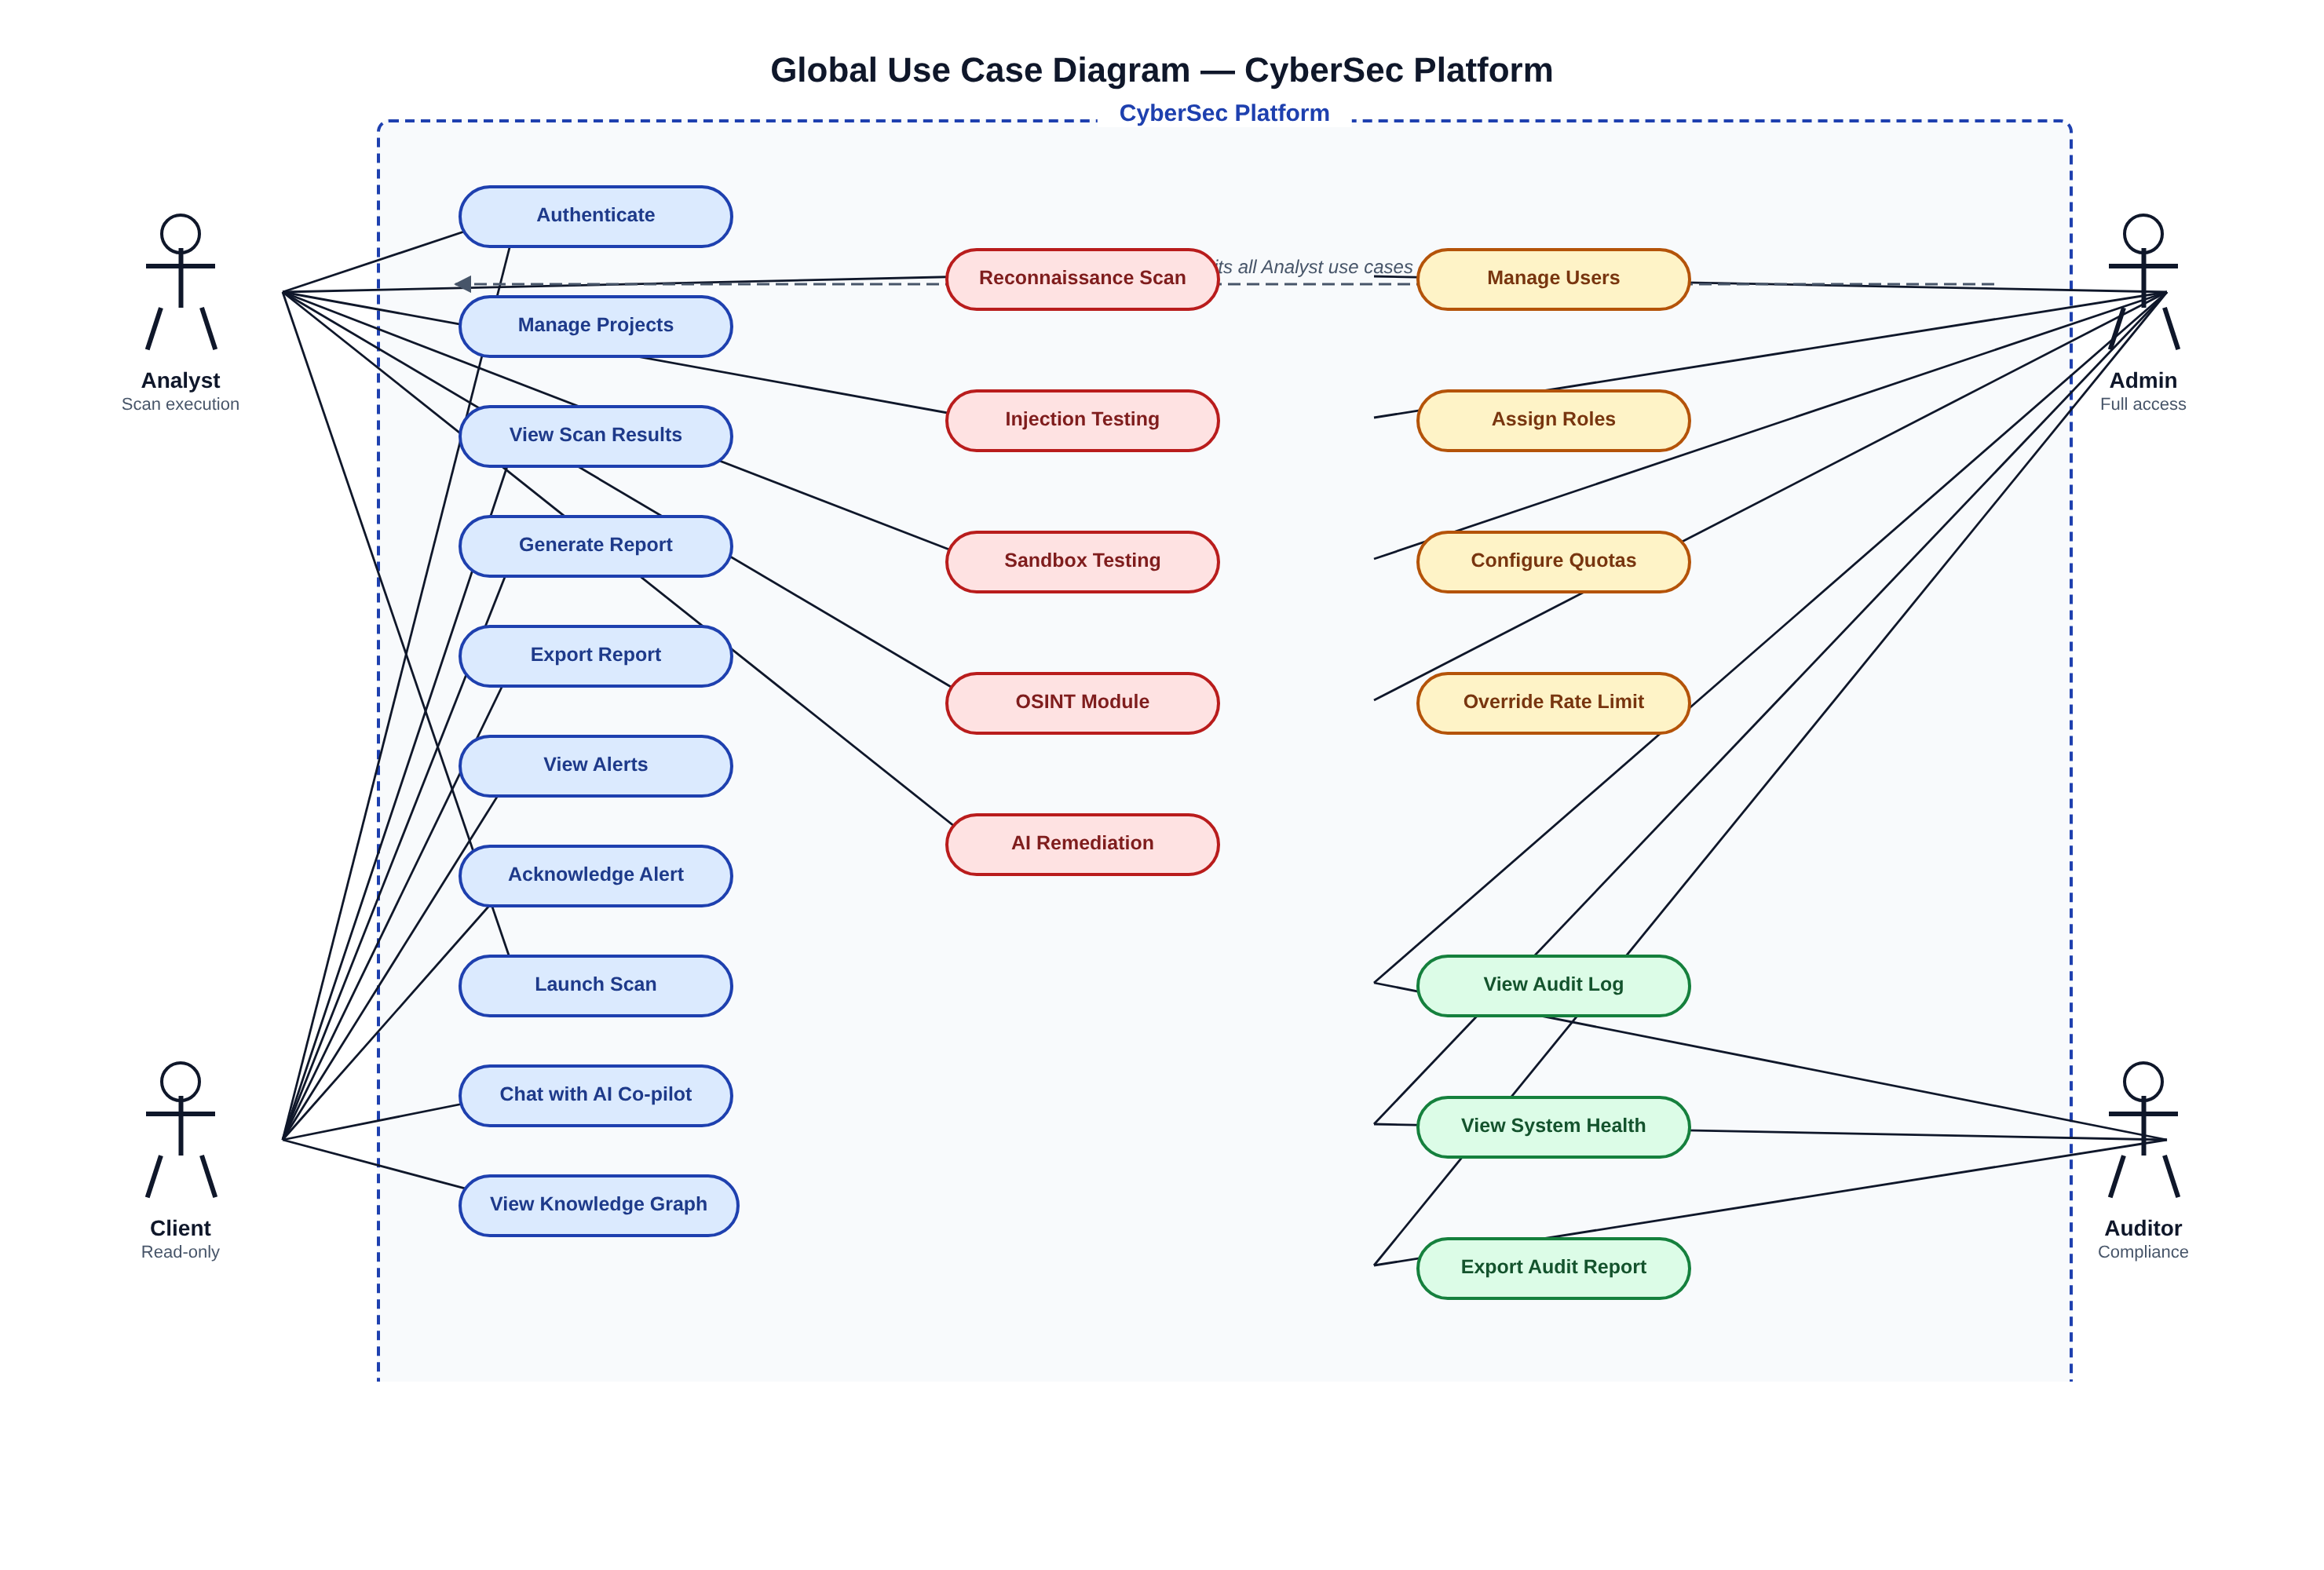
\includegraphics[width=0.82\textwidth]{img/usecase_global.png}
    \caption{Diagramme Global des Cas d'Utilisation -- Acteurs et Fonctionnalit\'es Cl\'es}
    \label{fig:usecase_global}
\end{figure}

\subsection{Cas d'Utilisation de l'Analyste de S\'ecurit\'e}
\par L'analyste configure les audits, explore les r\'esultats, manipule le graphe et valide les rem\'ediations.

\begin{figure}[!htbp]
    \centering
    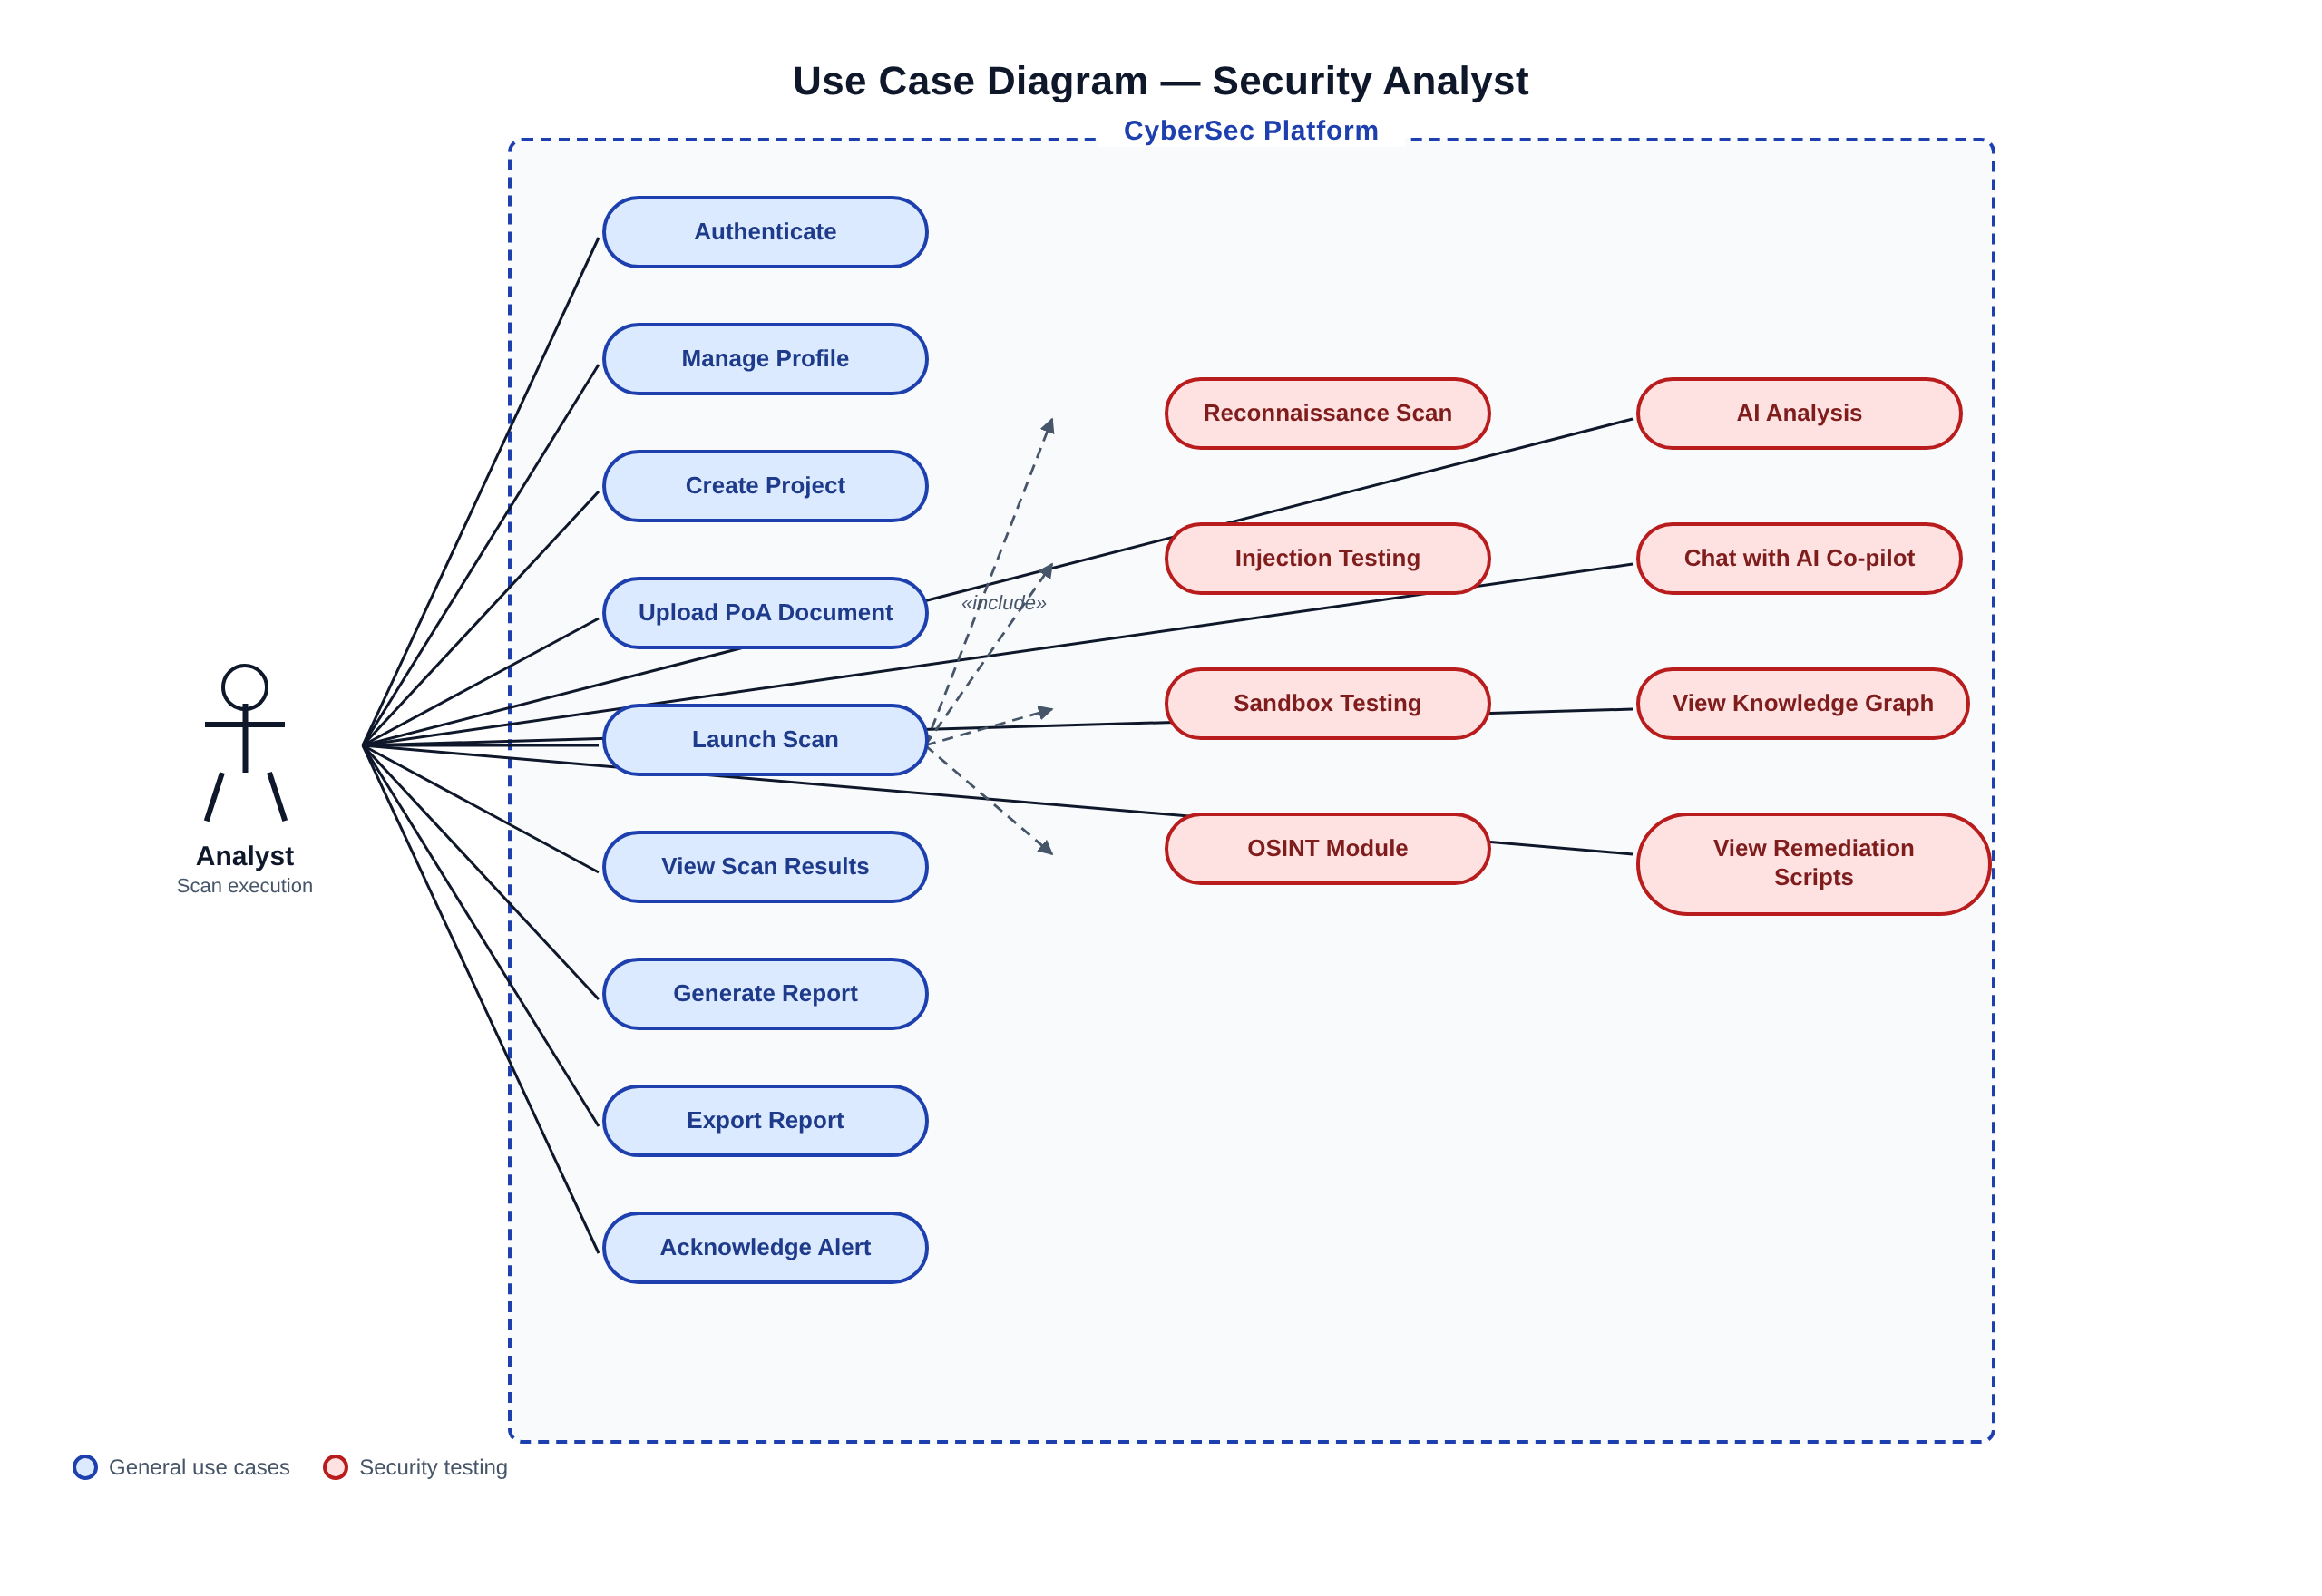
\includegraphics[width=0.82\textwidth]{img/usecase_analyst.png}
    \caption{Diagramme des Cas d'Utilisation -- Analyste de S\'ecurit\'e}
    \label{fig:usecase_analyst}
\end{figure}

\subsection{Cas d'Utilisation de l'Administrateur Syst\`eme}
\par L'administrateur g\`ere les privil\`eges, supervise la sant\'e des microservices et contr\^ole les pistes d'audit.

\begin{figure}[!htbp]
    \centering
    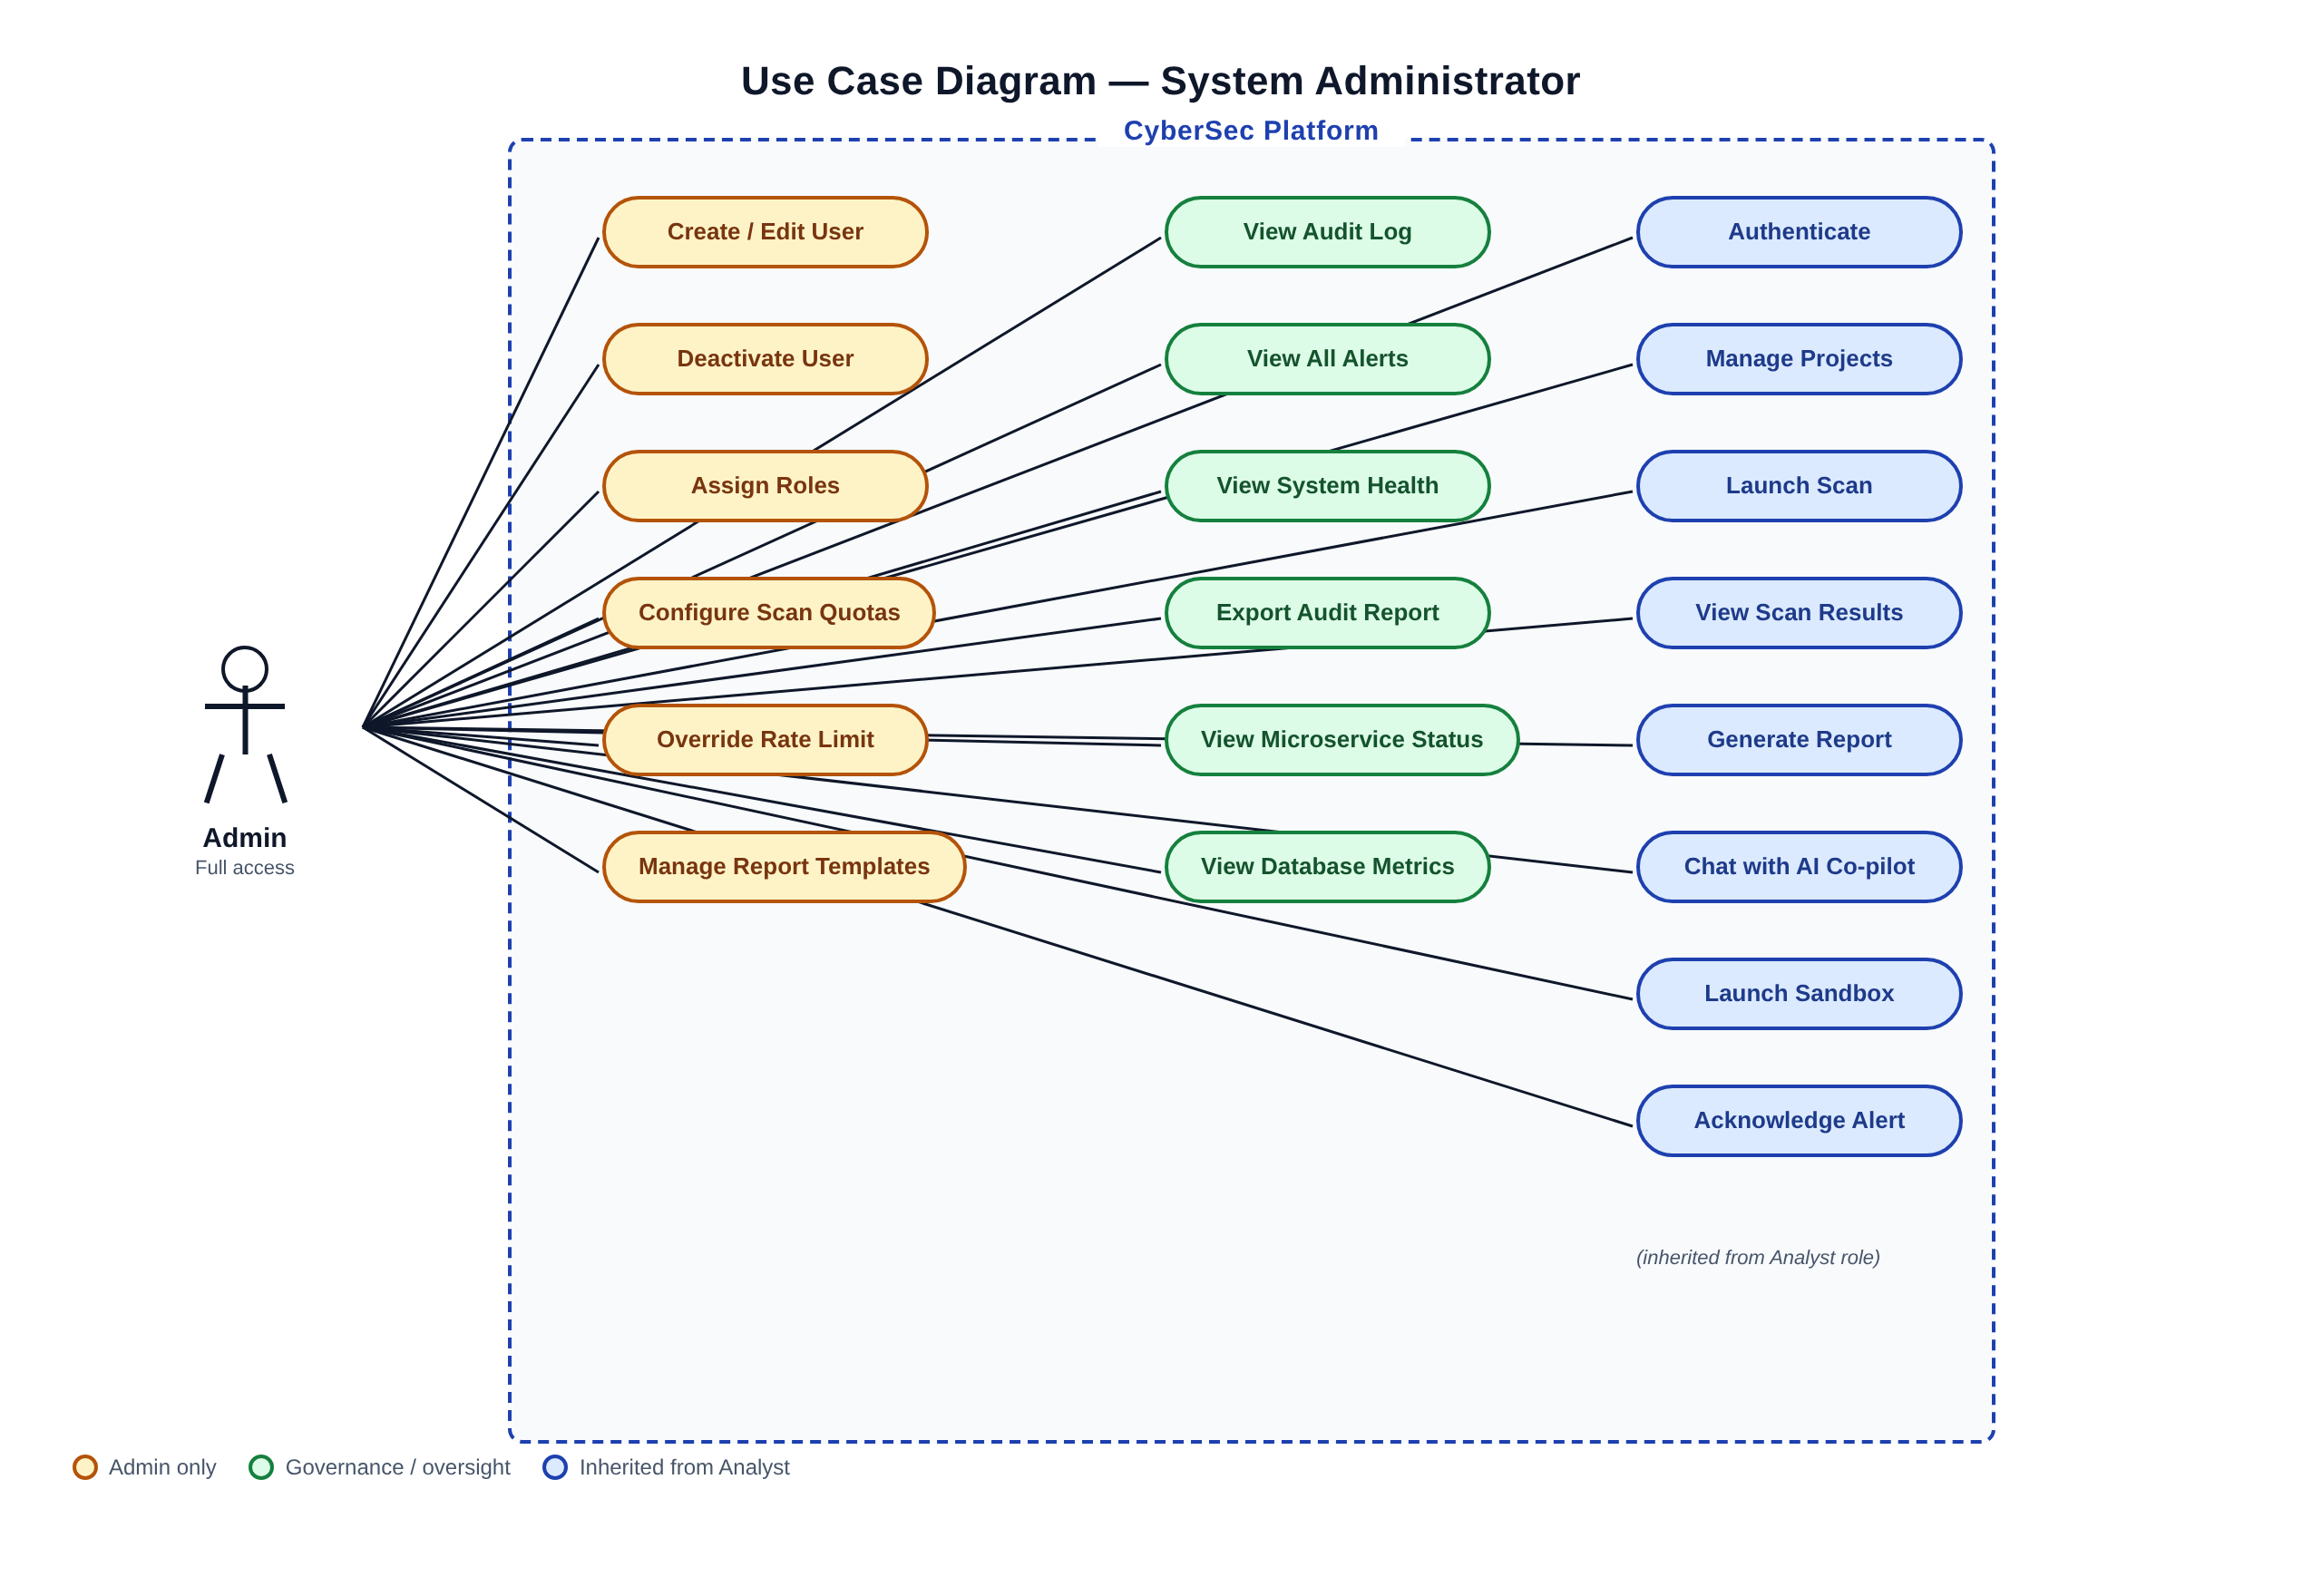
\includegraphics[width=0.82\textwidth]{img/usecase_admin.png}
    \caption{Diagramme des Cas d'Utilisation -- Administrateur Syst\`eme}
    \label{fig:usecase_admin}
\end{figure}

\subsection{Description Textuelle des Principaux Cas d'Utilisation}
\par \textbf{CU01 -- Lancement d'un Scan d'Audit :} L'analyste s\'electionne un projet et une cible, choisit le profil d'intensit\'e (Silent, Balanced, Aggressive), valide la pr\'esence de la PoA, et soumet la requ\^ete. Le back-end ins\`ere la commande dans Redis Streams et retourne un identifiant de session.
\par \textbf{CU02 -- G\'en\'eration de Remediation-as-Code :} L'analyste consulte un constat de vuln\'erabilit\'e et sollicite l'IA. Le microservice transmet le contexte technique \`a Ollama, r\'ecup\`ere le script structur\'e (Bash, Ansible, Dockerfile, Terraform) et l'affiche avec ses citations directes vers les logs bruts.

\section{Architecture Globale du Syst\`eme}
\subsection{Vue d'Ensemble du Syst\`eme}
\par La plateforme adopte une architecture microservices distribu\'ee et segment\'ee, assurant une s\'eparation nette des responsabilit\'es, une meilleure r\'esilience et une s\'ecurit\'e renforc\'ee par conception.

\subsection{Composants Applicatifs M\'etier (7 Composants Logiques)}
\par Sur le plan fonctionnel, l'application est r\'epartie en sept composants logiciels autonomes :
\begin{enumerate}
    \item \textbf{Back-end Web Applicatif (Laravel 11, Port 8000) :} Portail principal, gestion de l'authentification Sanctum, contr\^ole RBAC Spatie, mod\`ele ORM Eloquent, rendu des vues Blade et distribution des t\^aches vers les files de messages.
    \item \textbf{Microservice de Reconnaissance (Flask, Port 5000) :} Moteur d'ex\'ecution des scanners Nmap, Nuclei, Gobuster, Subfinder et WPScan, normalisation des r\'esultats (\texttt{ResultParser}) et initialisation de la topologie de graphe.
    \item \textbf{Microservice de S\'ecurit\'e Offensive (Flask, Port 5001) :} Modules d'\'evaluation des injections SQL/commandes/XSS, analyse de WAF et pilotage s\'ecuris\'e des bacs \`a sable conteneuris\'es.
    \item \textbf{Microservice OSINT (Flask, Port 5002) :} Renseignement passif (enregistrements DNS, requ\^etes WHOIS, certificats SSL/TLS via \texttt{crt.sh}, d\'etection d'empreintes technologiques).
    \item \textbf{Microservice d'IA Contrainte (Flask, Port 5003) :} Couche d'assistance intelligente connect\'ee au mod\`ele local \texttt{qwen2.5-coder} via Ollama pour la production de Remediation-as-Code.
    \item \textbf{Passerelle d'API (API Gateway, Flask, Port 8080) :} Point d'entr\'ee et routeur interne vers les microservices, assurant le contr\^ole de d\'ebit (\textit{rate limiting}) et la tra\c{c}abilit\'e par \texttt{X-Correlation-ID}.
    \item \textbf{Worker Asynchrone (Python) :} Processus d'arri\`ere-plan consommant les \'ev\'enements de scan via \texttt{XREADGROUP} sur Redis Streams, coordonnant les t\^aches longues et persistant les constats dans PostgreSQL.
\end{enumerate}

\subsection{Conteneurs d'Infrastructure Docker (12 Services Conteneuris\'es)}
\par Sur le plan infrastructurel, le d\'eploiement orchestre douze conteneurs Docker compl\'ementaires :
\begin{itemize}
    \item Les 7 conteneurs h\'ebergeant les 7 composants applicatifs d\'ecrits ci-dessus.
    \item \textbf{8. Nginx 1.27 :} Serveur mandataire inverse (\textit{reverse proxy}) assurant la terminaison TLS 1.3 et le durcissement des en-t\^etes HTTP.
    \item \textbf{9. PostgreSQL 16 + Apache AGE :} Syst\`eme de gestion de base de donn\'ees unifi\'e relationnel (14 tables) et graphe openCypher.
    \item \textbf{10. Redis 7 :} Magasin de donn\'ees en m\'emoire servant de Message Broker Streams, cache applicatif et gestionnaire de sessions.
    \item \textbf{11. Ollama :} Serveur d'inf\'erence local ex\'ecutant le mod\`ele d\'edi\'e au code \texttt{qwen2.5-coder}.
    \item \textbf{12. Docker-Socket-Proxy :} Proxy de s\'ecurit\'e interdisant les acc\`es directs au socket Unix de Docker pour pr\'evenir toute \'evasion de conteneur.
\end{itemize}

\begin{figure}[!htbp]
    \centering
    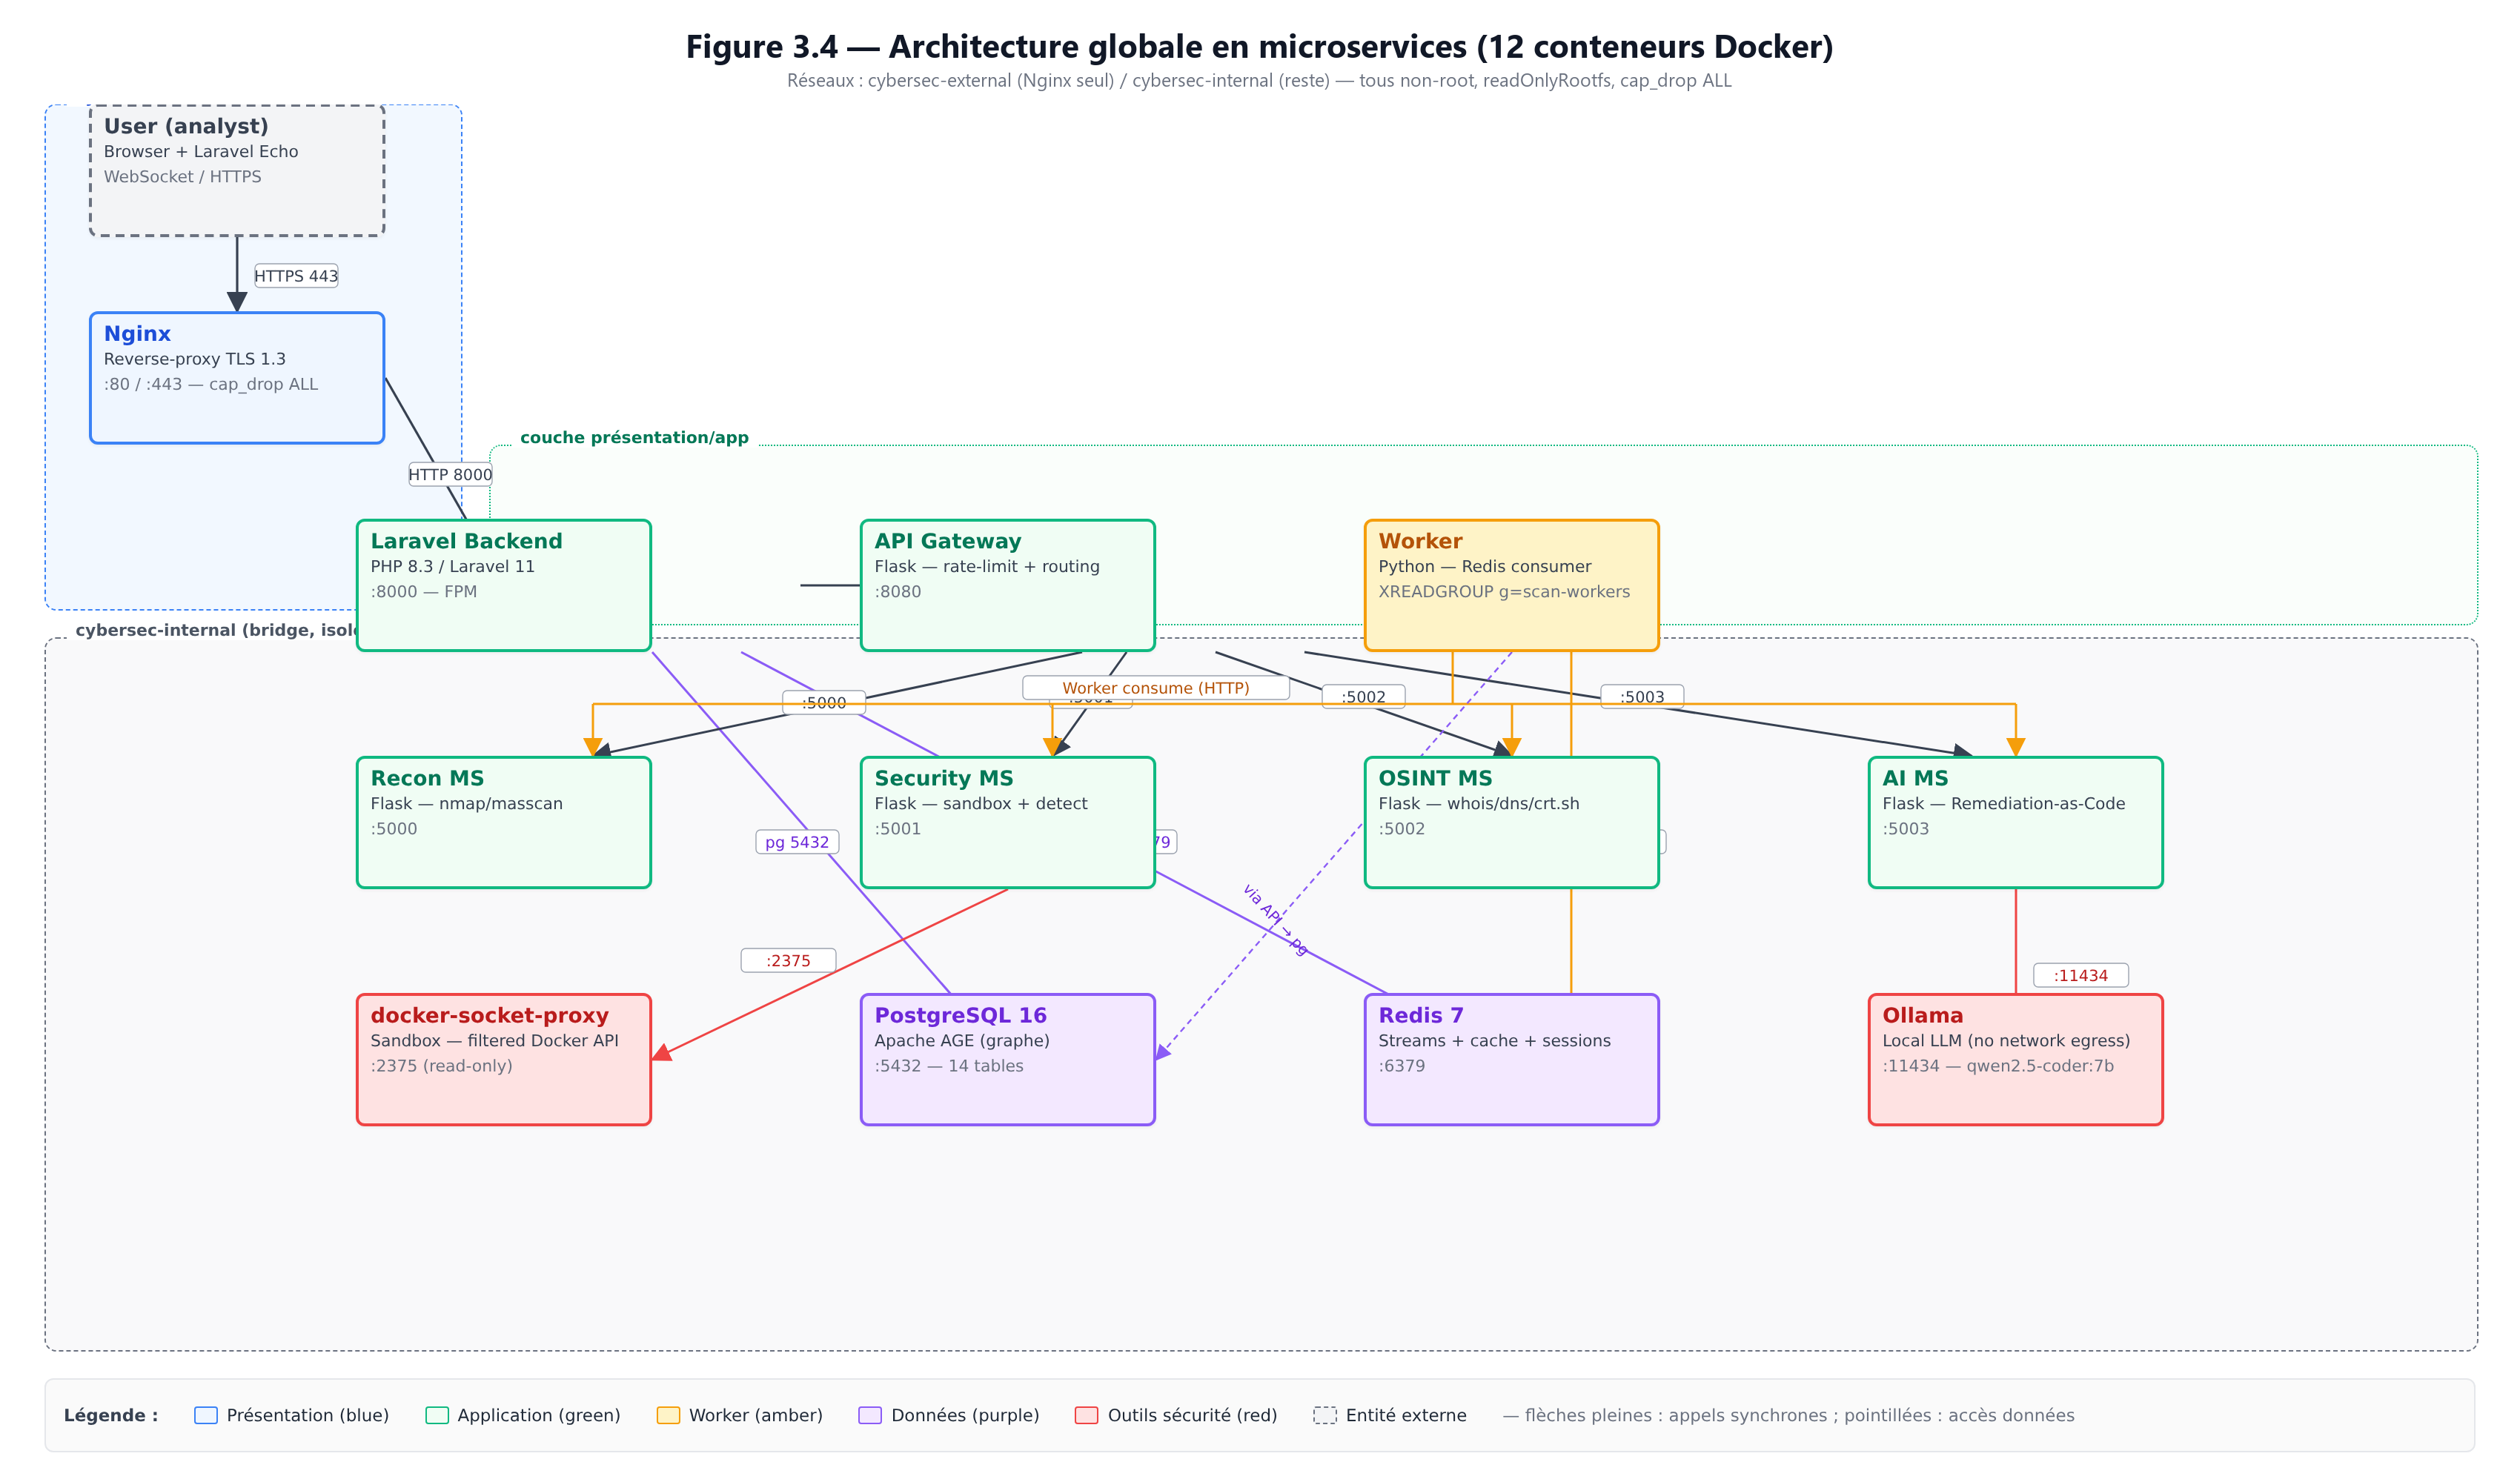
\includegraphics[width=0.92\textwidth]{img/component_diagram.png}
    \caption{Architecture Globale en Microservices -- Vue des 12 Conteneurs Docker et R\'eseaux Segment\'es}
    \label{fig:component_diagram}
\end{figure}

\subsection{Communication Inter-Services}
\par La figure~\ref{fig:ms_comms} pr\'esente la cartographie des flux d'\'echanges internes : requ\^etes REST synchrones, streaming d'\'ev\'enements asynchrones et notifications de mise \`a jour.

\begin{figure}[!htbp]
\centering
\begin{tikzpicture}[
    node distance=8mm and 14mm,
    box/.style={draw, rounded corners=2pt, fill=blue!8, draw=blue!50, thick, minimum width=28mm, minimum height=8mm, align=center, font=\footnotesize},
    sync/.style={-{Stealth[length=2mm]}, thick, draw=green!60!black},
    async/.style={-{Stealth[length=2mm]}, thick, dashed, draw=orange!80!black},
    notify/.style={-{Stealth[length=2mm]}, thick, dotted, draw=red!70!black},
]
\node[box] (browser) {Navigateur (Blade)};
\node[box, right=of browser] (laravel) {Back-end\\Laravel 11};
\node[box, above right=4mm and 16mm of laravel] (recon) {MS Recon\\(Flask :5000)};
\node[box, right=of laravel] (gateway) {Passerelle API\\(Flask :8080)};
\node[box, below right=4mm and 16mm of laravel] (ai) {MS IA\\(Flask :5003)};
\node[box, right=of gateway] (redis) {Redis 7\\Streams};
\node[box, below=of redis] (worker) {Worker\\(Python)};
\node[box, below=of laravel] (pg) {PostgreSQL 16\\+ Apache AGE};
\draw[sync] (browser) -- node[above, font=\tiny]{REST/HTTPS} (laravel);
\draw[sync] (laravel) -- node[above, font=\tiny]{REST} (gateway);
\draw[sync] (gateway) -- (recon);
\draw[sync] (gateway) -- (ai);
\draw[async] (laravel) -- node[right, font=\tiny]{XADD} (redis);
\draw[async] (redis) -- node[right, font=\tiny]{XREADGROUP} (worker);
\draw[async] (worker) -- node[below, font=\tiny]{r\'esultats} (pg);
\draw[notify] (pg) -- node[left, font=\tiny]{NOTIFY} (laravel);
\draw[notify] (recon) -- node[below, font=\tiny]{insert} (pg);
\end{tikzpicture}
\caption{Flux de Communication du Traitement Asynchrone d'un Scan -- REST Synchrone, Redis Streams et PostgreSQL NOTIFY}
\label{fig:ms_comms}
\end{figure}

\subsection{Communication Synchrone REST vs Asynchrone par \'Ev\'enements}
\par La plateforme combine deux paradigmes d'\'echange compl\'ementaires :
\begin{itemize}
    \item \textbf{Communication synchrone REST (HTTP/JSON) :} R\'eserv\'ee aux requ\^etes imm\'ediates (interrogation du tableau de bord, requ\^etes OSINT rapides, inf\'erence de dialogue IA).
    \item \textbf{Communication asynchrone (Redis Streams) :} Utilis\'ee pour l'ex\'ecution des scanners lourds. Le back-end publie un message (\texttt{XADD}), imm\'ediatement acquitt\'e pour l'utilisateur, tandis que le worker d\'epile le travail en arri\`ere-plan sans bloquer l'IHM.
\end{itemize}

\section{Conception des Donn\'ees et Dynamique du Syst\`eme}
\subsection{Mod\`ele Entit\'e-Association (ERD)}
\par La base de donn\'ees structure 14 tables relationnelles li\'ees par des contraintes d'int\'egrit\'e r\'ef\'erentielle strictes et enrichies de colonnes \texttt{JSONB} index\'ees par index GIN.

\begin{figure}[!htbp]
    \centering
    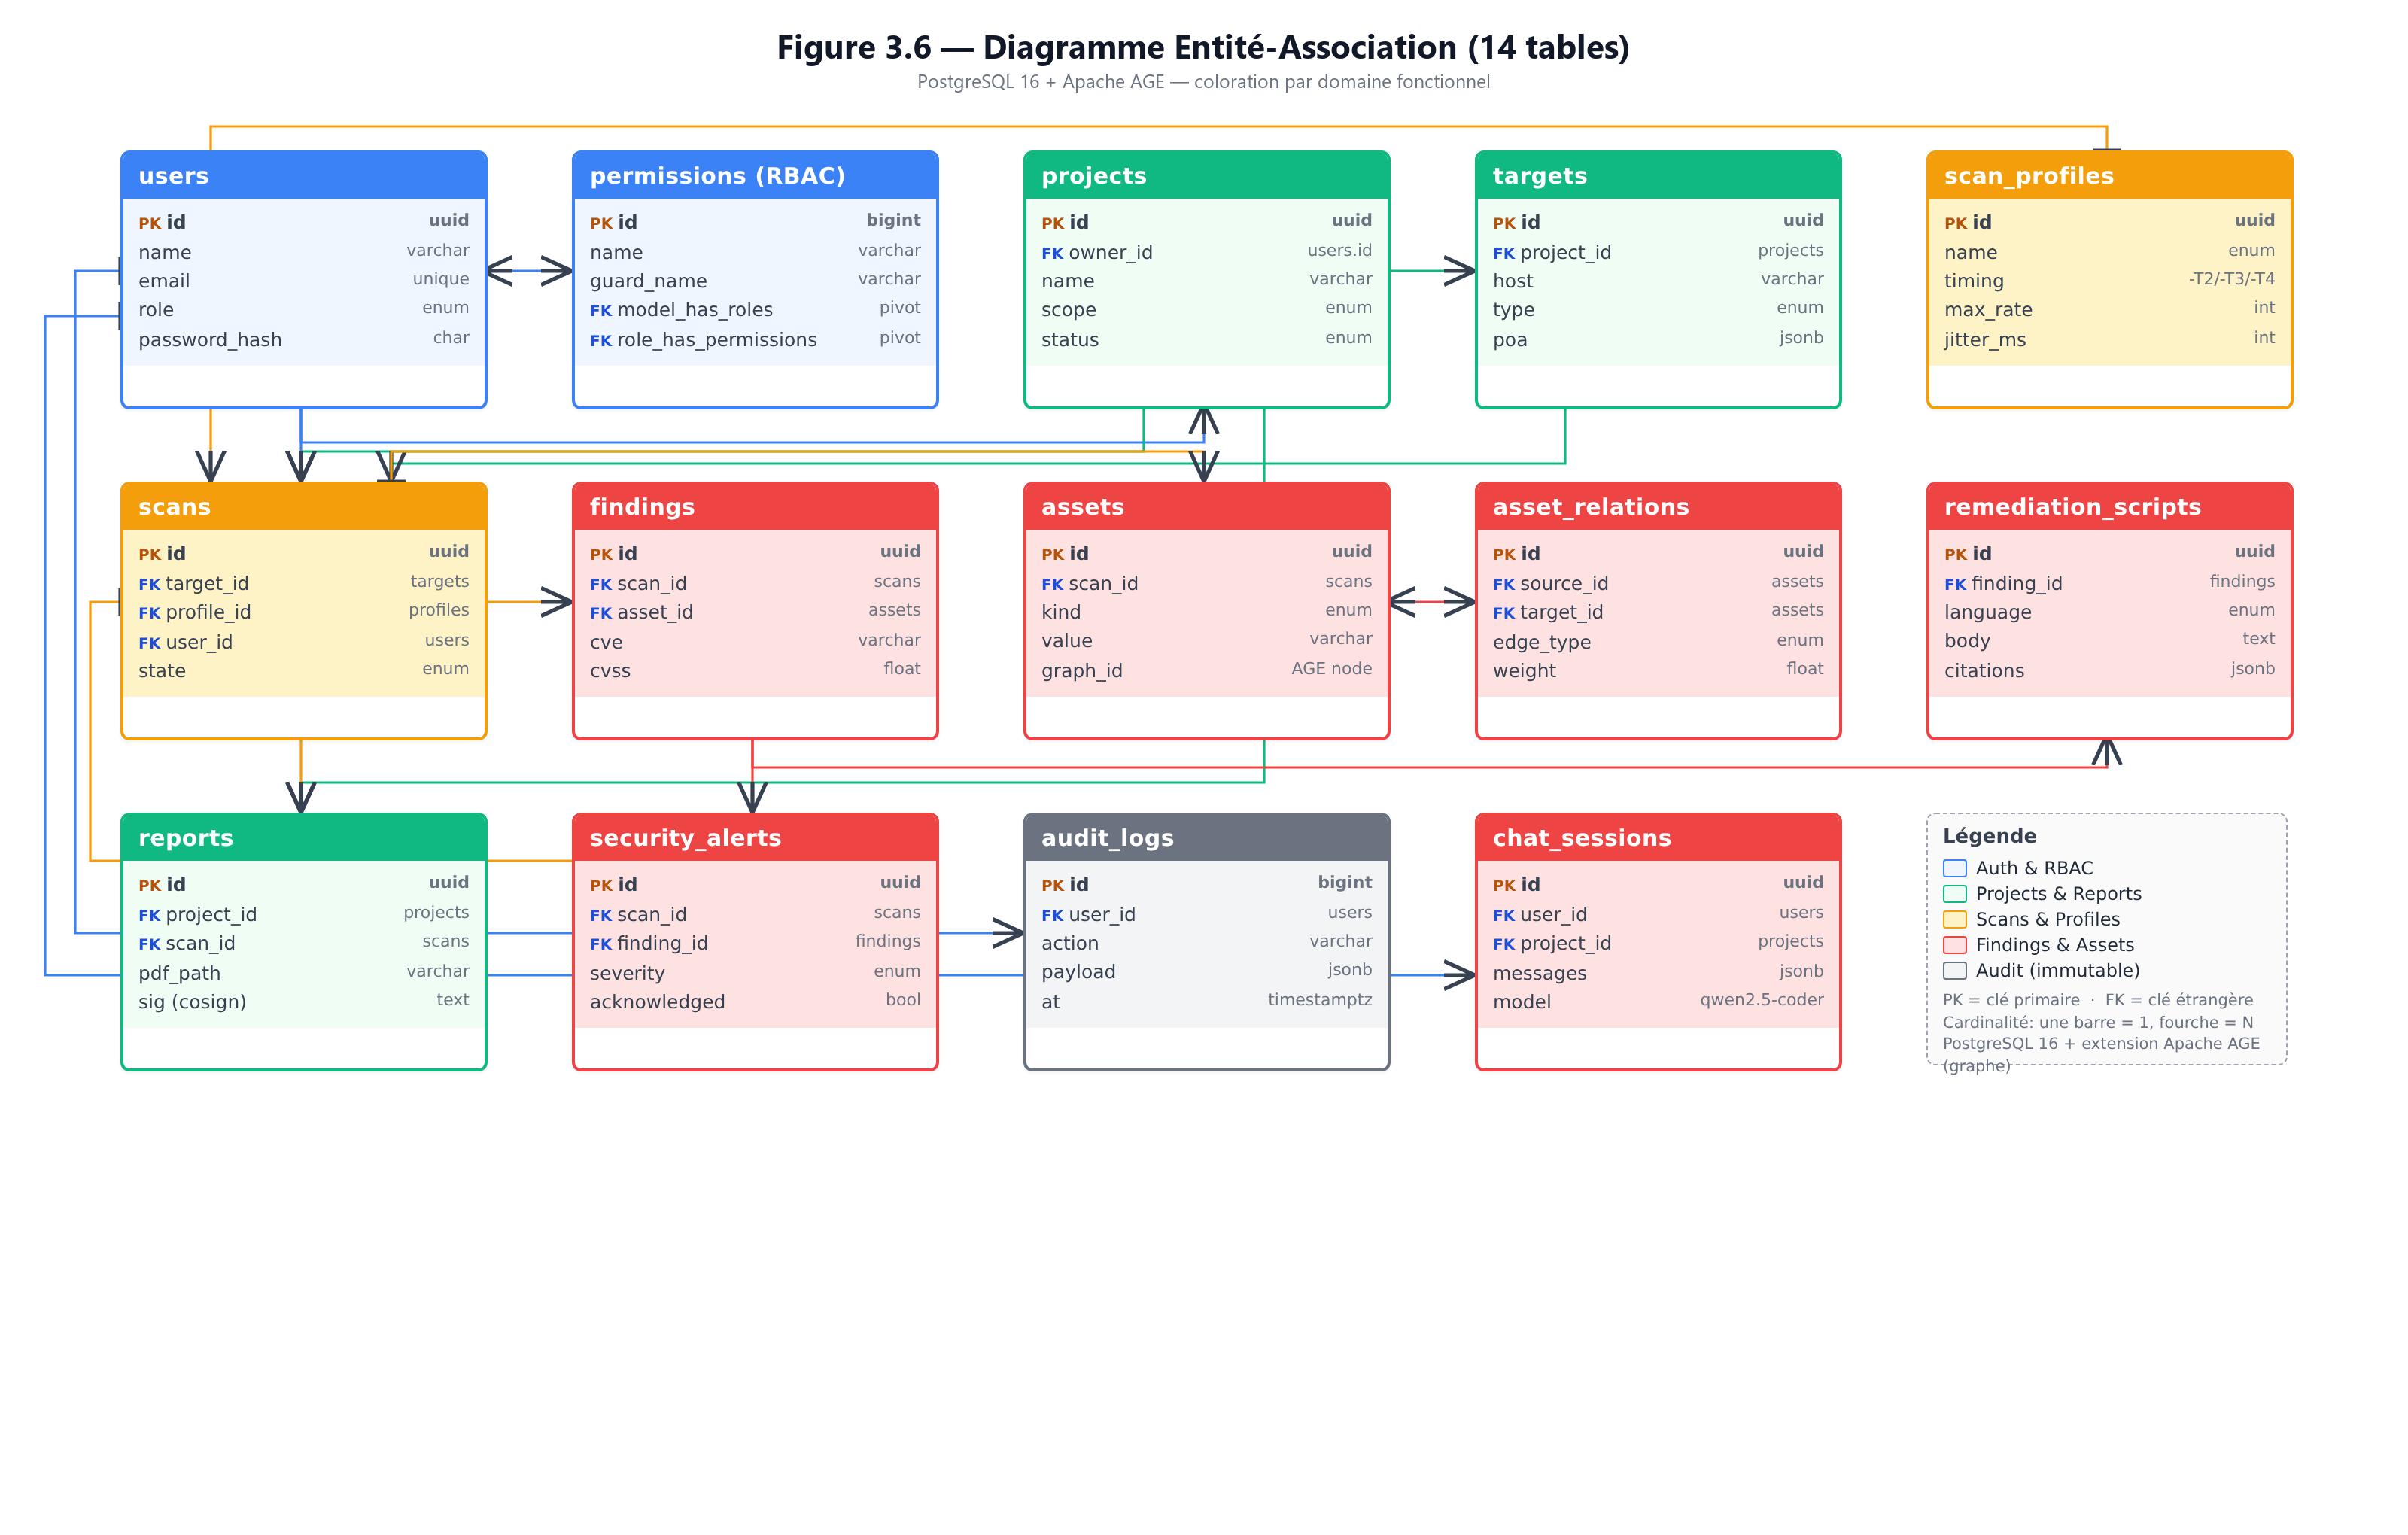
\includegraphics[width=0.92\textwidth]{img/erd.png}
    \caption{Mod\`ele Entit\'e-Association (ERD) -- Les 14 Tables de la Plateforme}
    \label{fig:erd_diagram}
\end{figure}

\subsection{Diagramme de Classes du Mod\`ele de Donn\'ees}
\par Tandis que le Mod\`ele Entit\'e-Association (ERD) formalise la structure relationnelle et physique de la base de donn\'ees, le diagramme de classes repr\'esente la structure logique des principales entit\'es m\'etier et leurs relations au sein du framework applicatif. La structure objet et les relations cardinales entre les entit\'es sont illustr\'ees dans la figure~\ref{fig:class_diagram}.

\begin{figure}[!htbp]
    \centering
    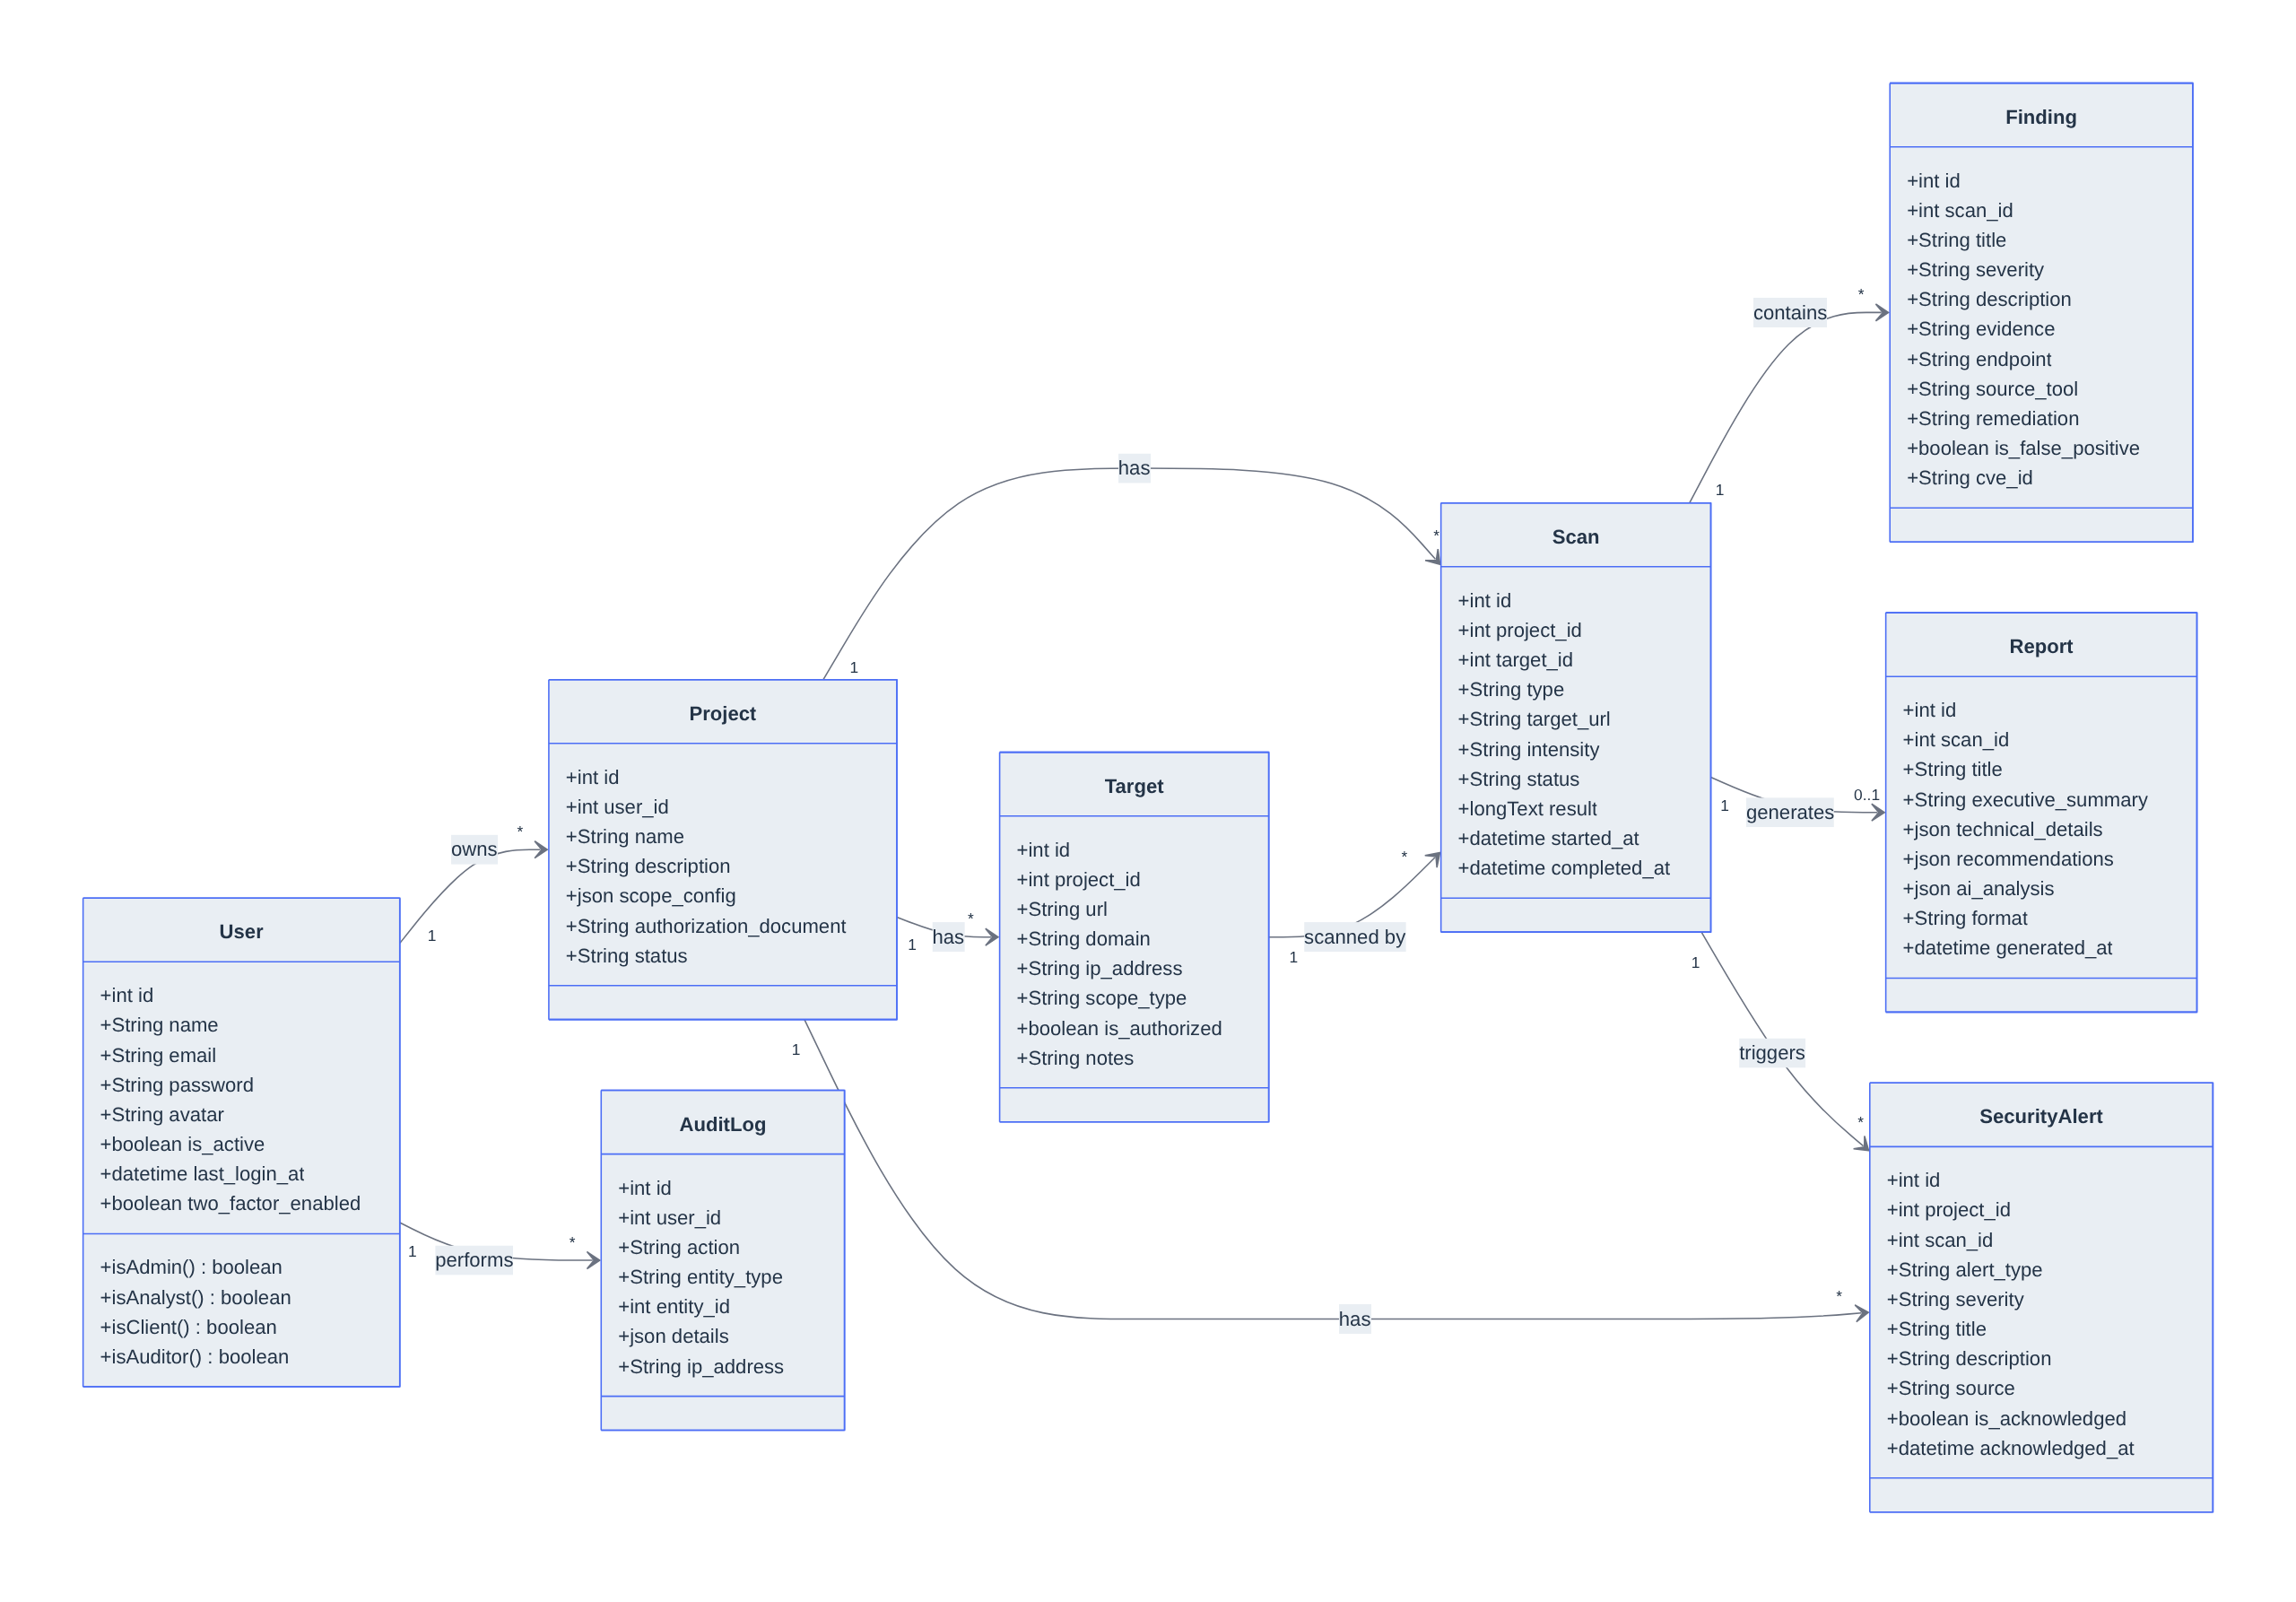
\includegraphics[width=0.90\textwidth]{img/class_diagram.png}
    \caption{Diagramme de Classes -- Entit\'es M\'etier et Relations du Mod\`ele}
    \label{fig:class_diagram}
\end{figure}

\subsection{Mod\`ele du Graphe de Connaissances et Projection Apache AGE}
\par Les relations de s\'ecurit\'e sont mod\'elis\'ees sous forme de n\oe uds (\textit{Target}, \textit{Asset}, \textit{Port}, \textit{Service}, \textit{Vulnerability}) et d'ar\^etes typ\'ees (\textit{RESOLVES\_TO}, \textit{HOSTS}, \textit{RUNS}, \textit{HAS\_VULN}, \textit{IMPACTS}). Cette mod\'elisation permet de calculer le rayon d'impact (\textit{blast radius}) par parcours de graphe en largeur (BFS) impl\'ement\'e sous NetworkX.

\subsection{Diagramme de S\'equence du D\'eroulement d'un Scan}
\par La figure~\ref{fig:sequence_scan} mod\'elise la s\'equence d'ex\'ecution compl\`ete d'un audit de reconnaissance, de la soumission initiale jusqu'\`a la persistance des constats et \`a l'analyse IA.

\begin{figure}[!htbp]
    \centering
    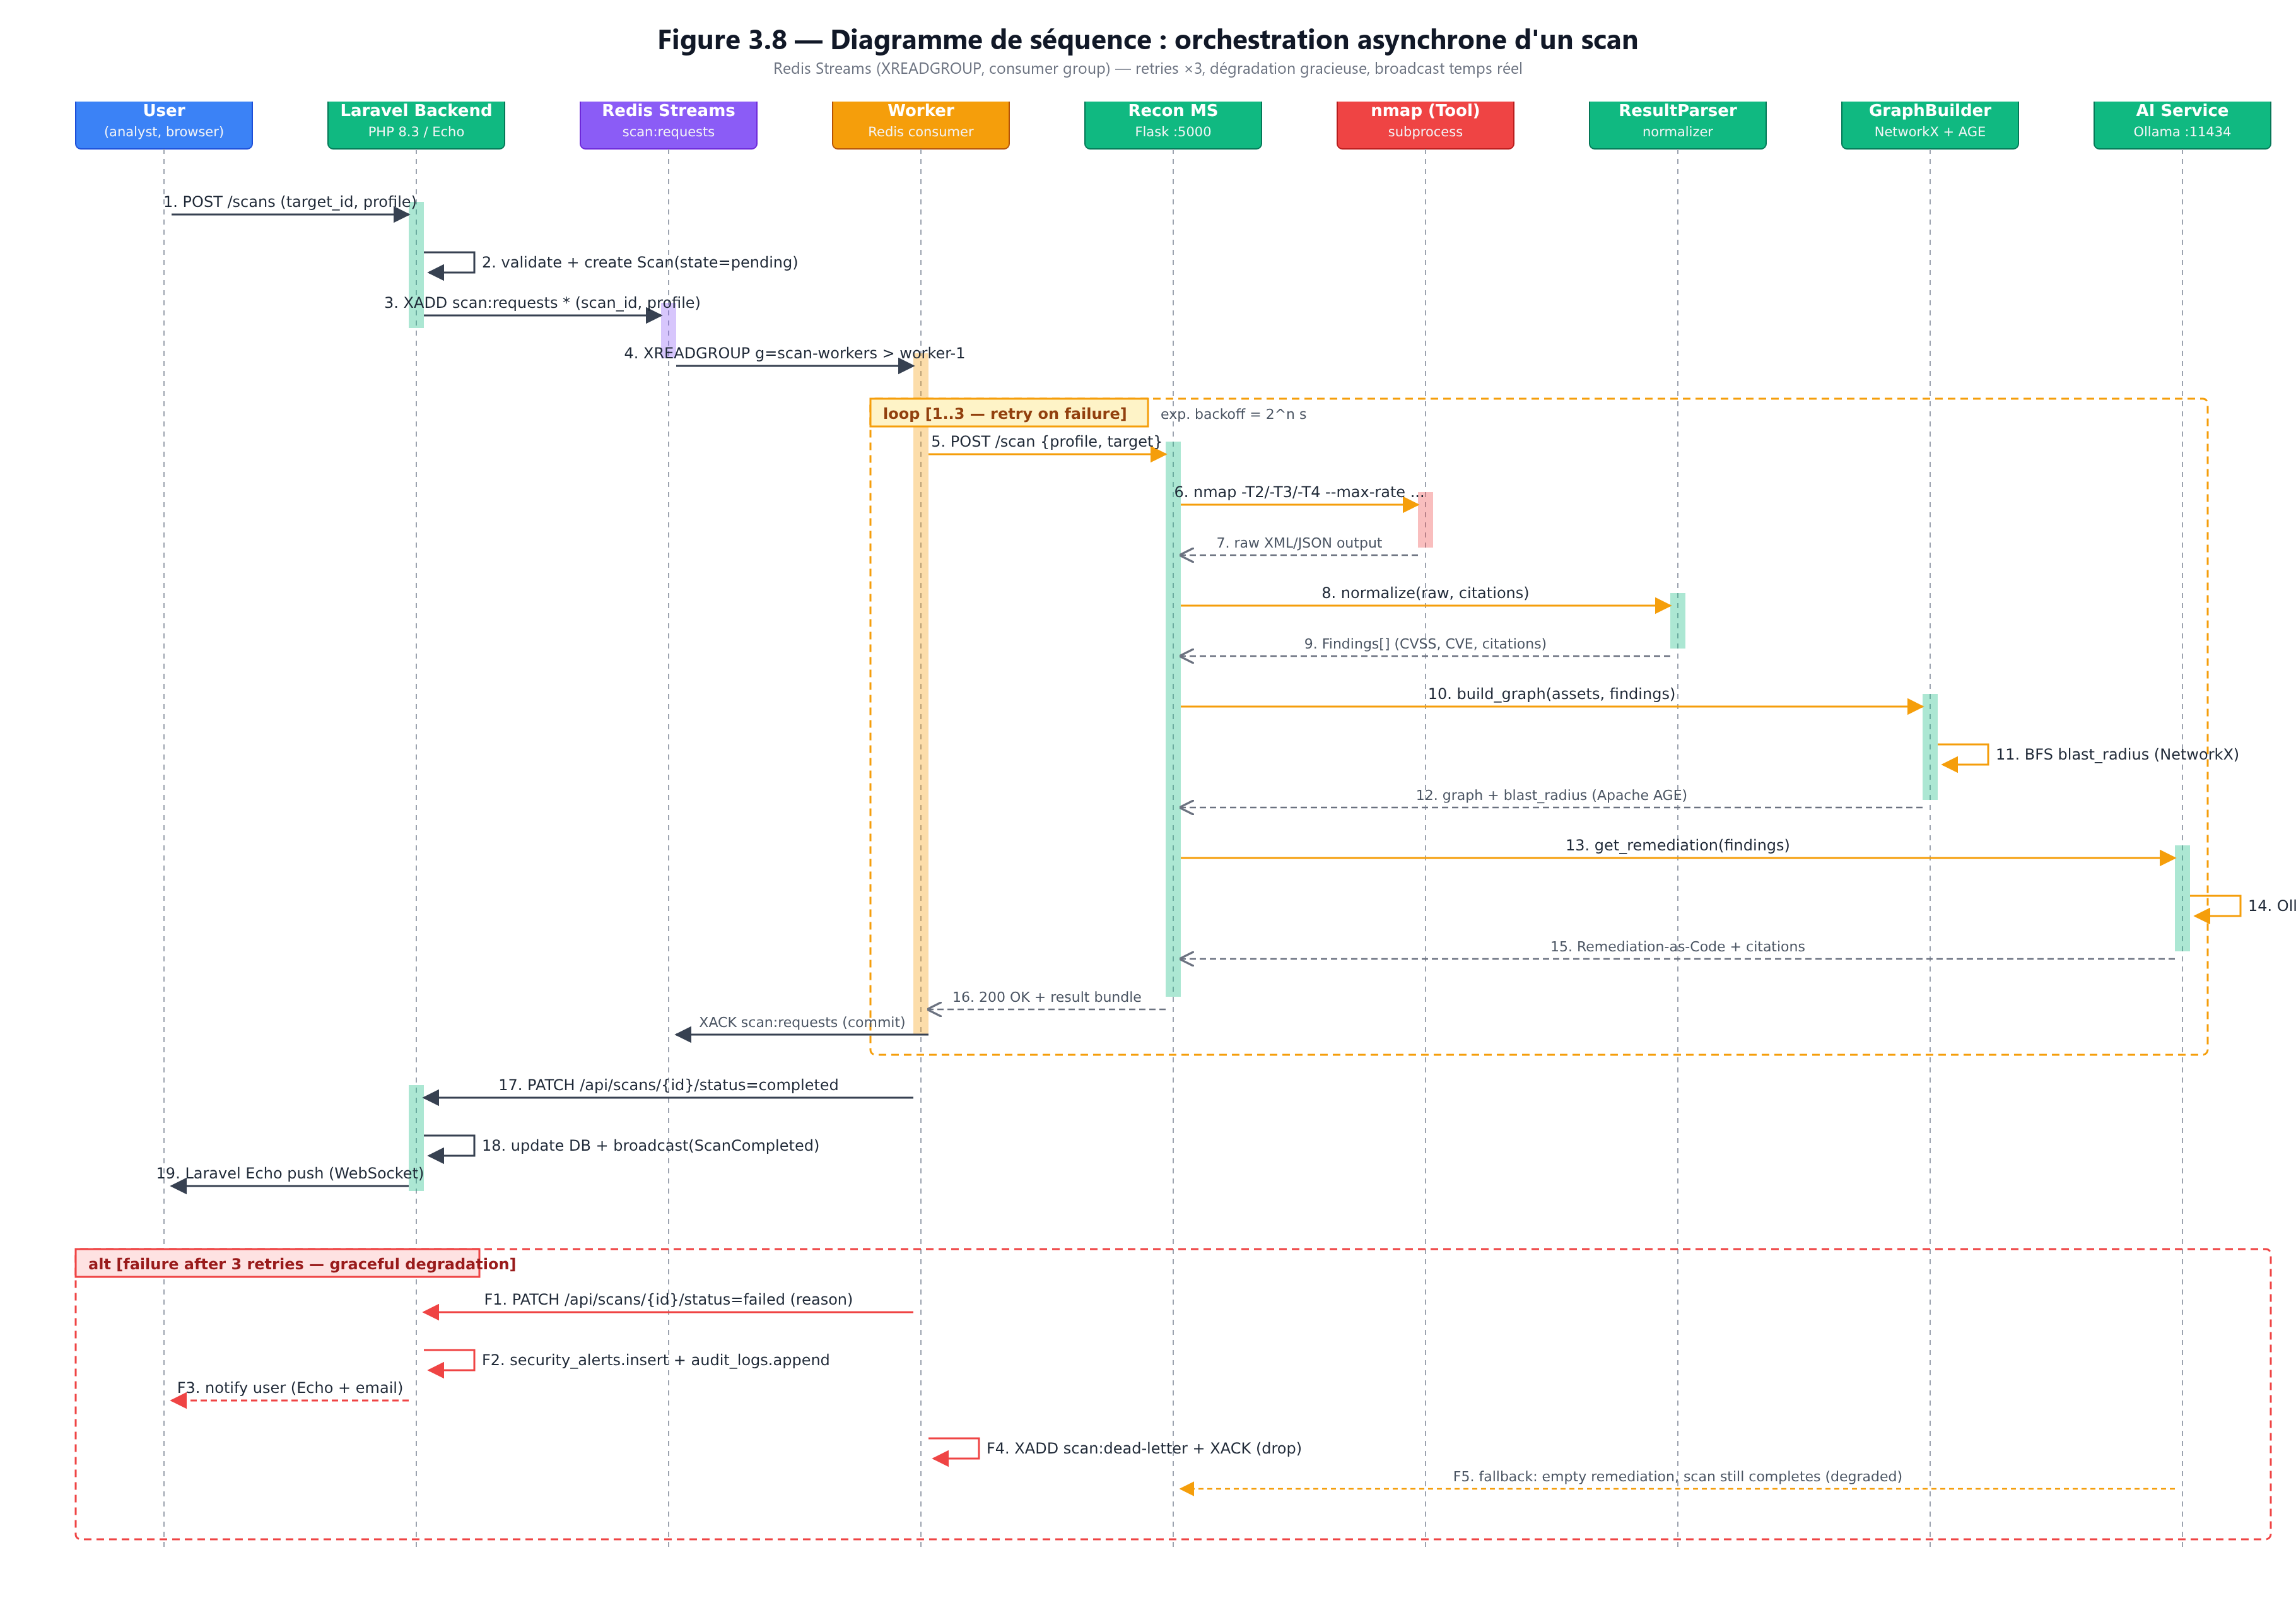
\includegraphics[width=0.92\textwidth]{img/sequence_scan.png}
    \caption{Diagramme de S\'equence -- Orchestration Asynchrone d'un Scan}
    \label{fig:sequence_scan}
\end{figure}

\subsection{Machine \`a \'Etats d'un Scan}
\par Le cycle de vie d'une t\^ache de scan est r\'egi par une machine \`a \'etats finis d\'eterministe comprenant les \'etats \texttt{Pending}, \texttt{Queued}, \texttt{Running}, \texttt{Completed}, \texttt{Failed} et \texttt{Cancelled}.

\begin{figure}[!htbp]
    \centering
    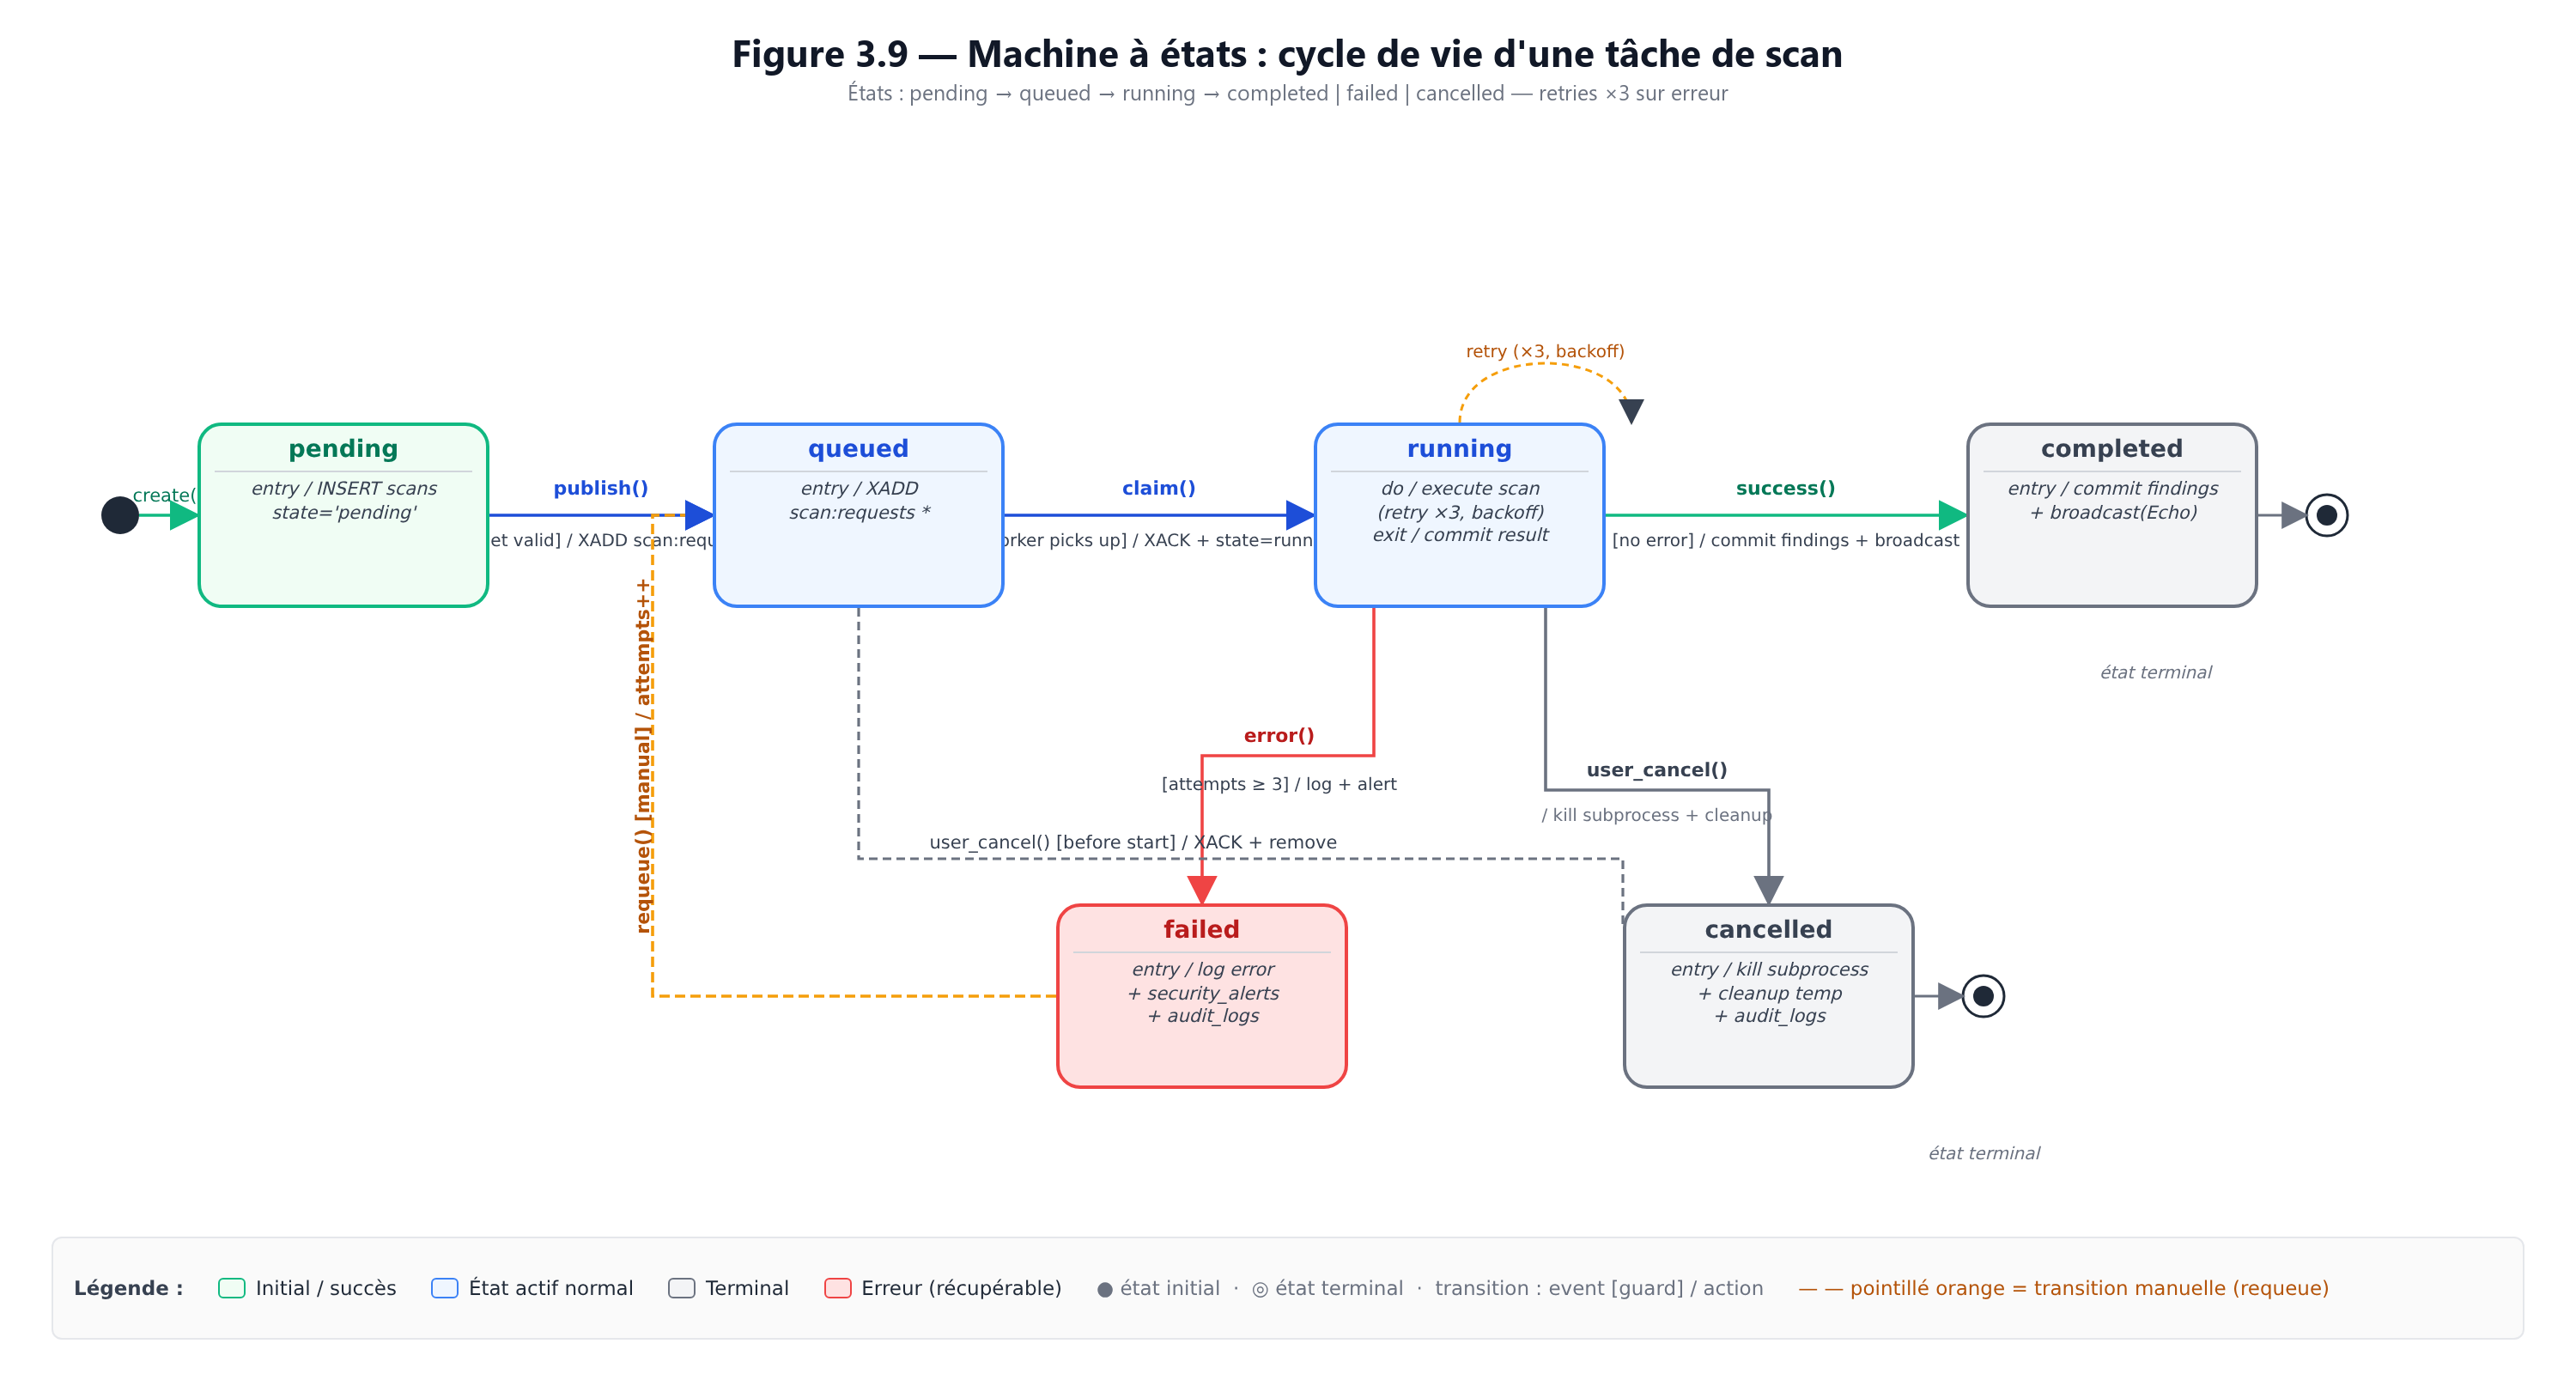
\includegraphics[width=0.85\textwidth]{img/state_machine.png}
    \caption{Machine \`a \'Etats -- Cycle de Vie d'une T\^ache de Scan}
    \label{fig:state_machine}
\end{figure}

\subsection{Diagramme de Flux de Donn\'ees (DFD)}
\par Le cheminement et les transformations successives des donn\'ees sont synth\'etis\'es dans le diagramme de flux de la figure~\ref{fig:data_flow}.

\begin{figure}[!htbp]
    \centering
    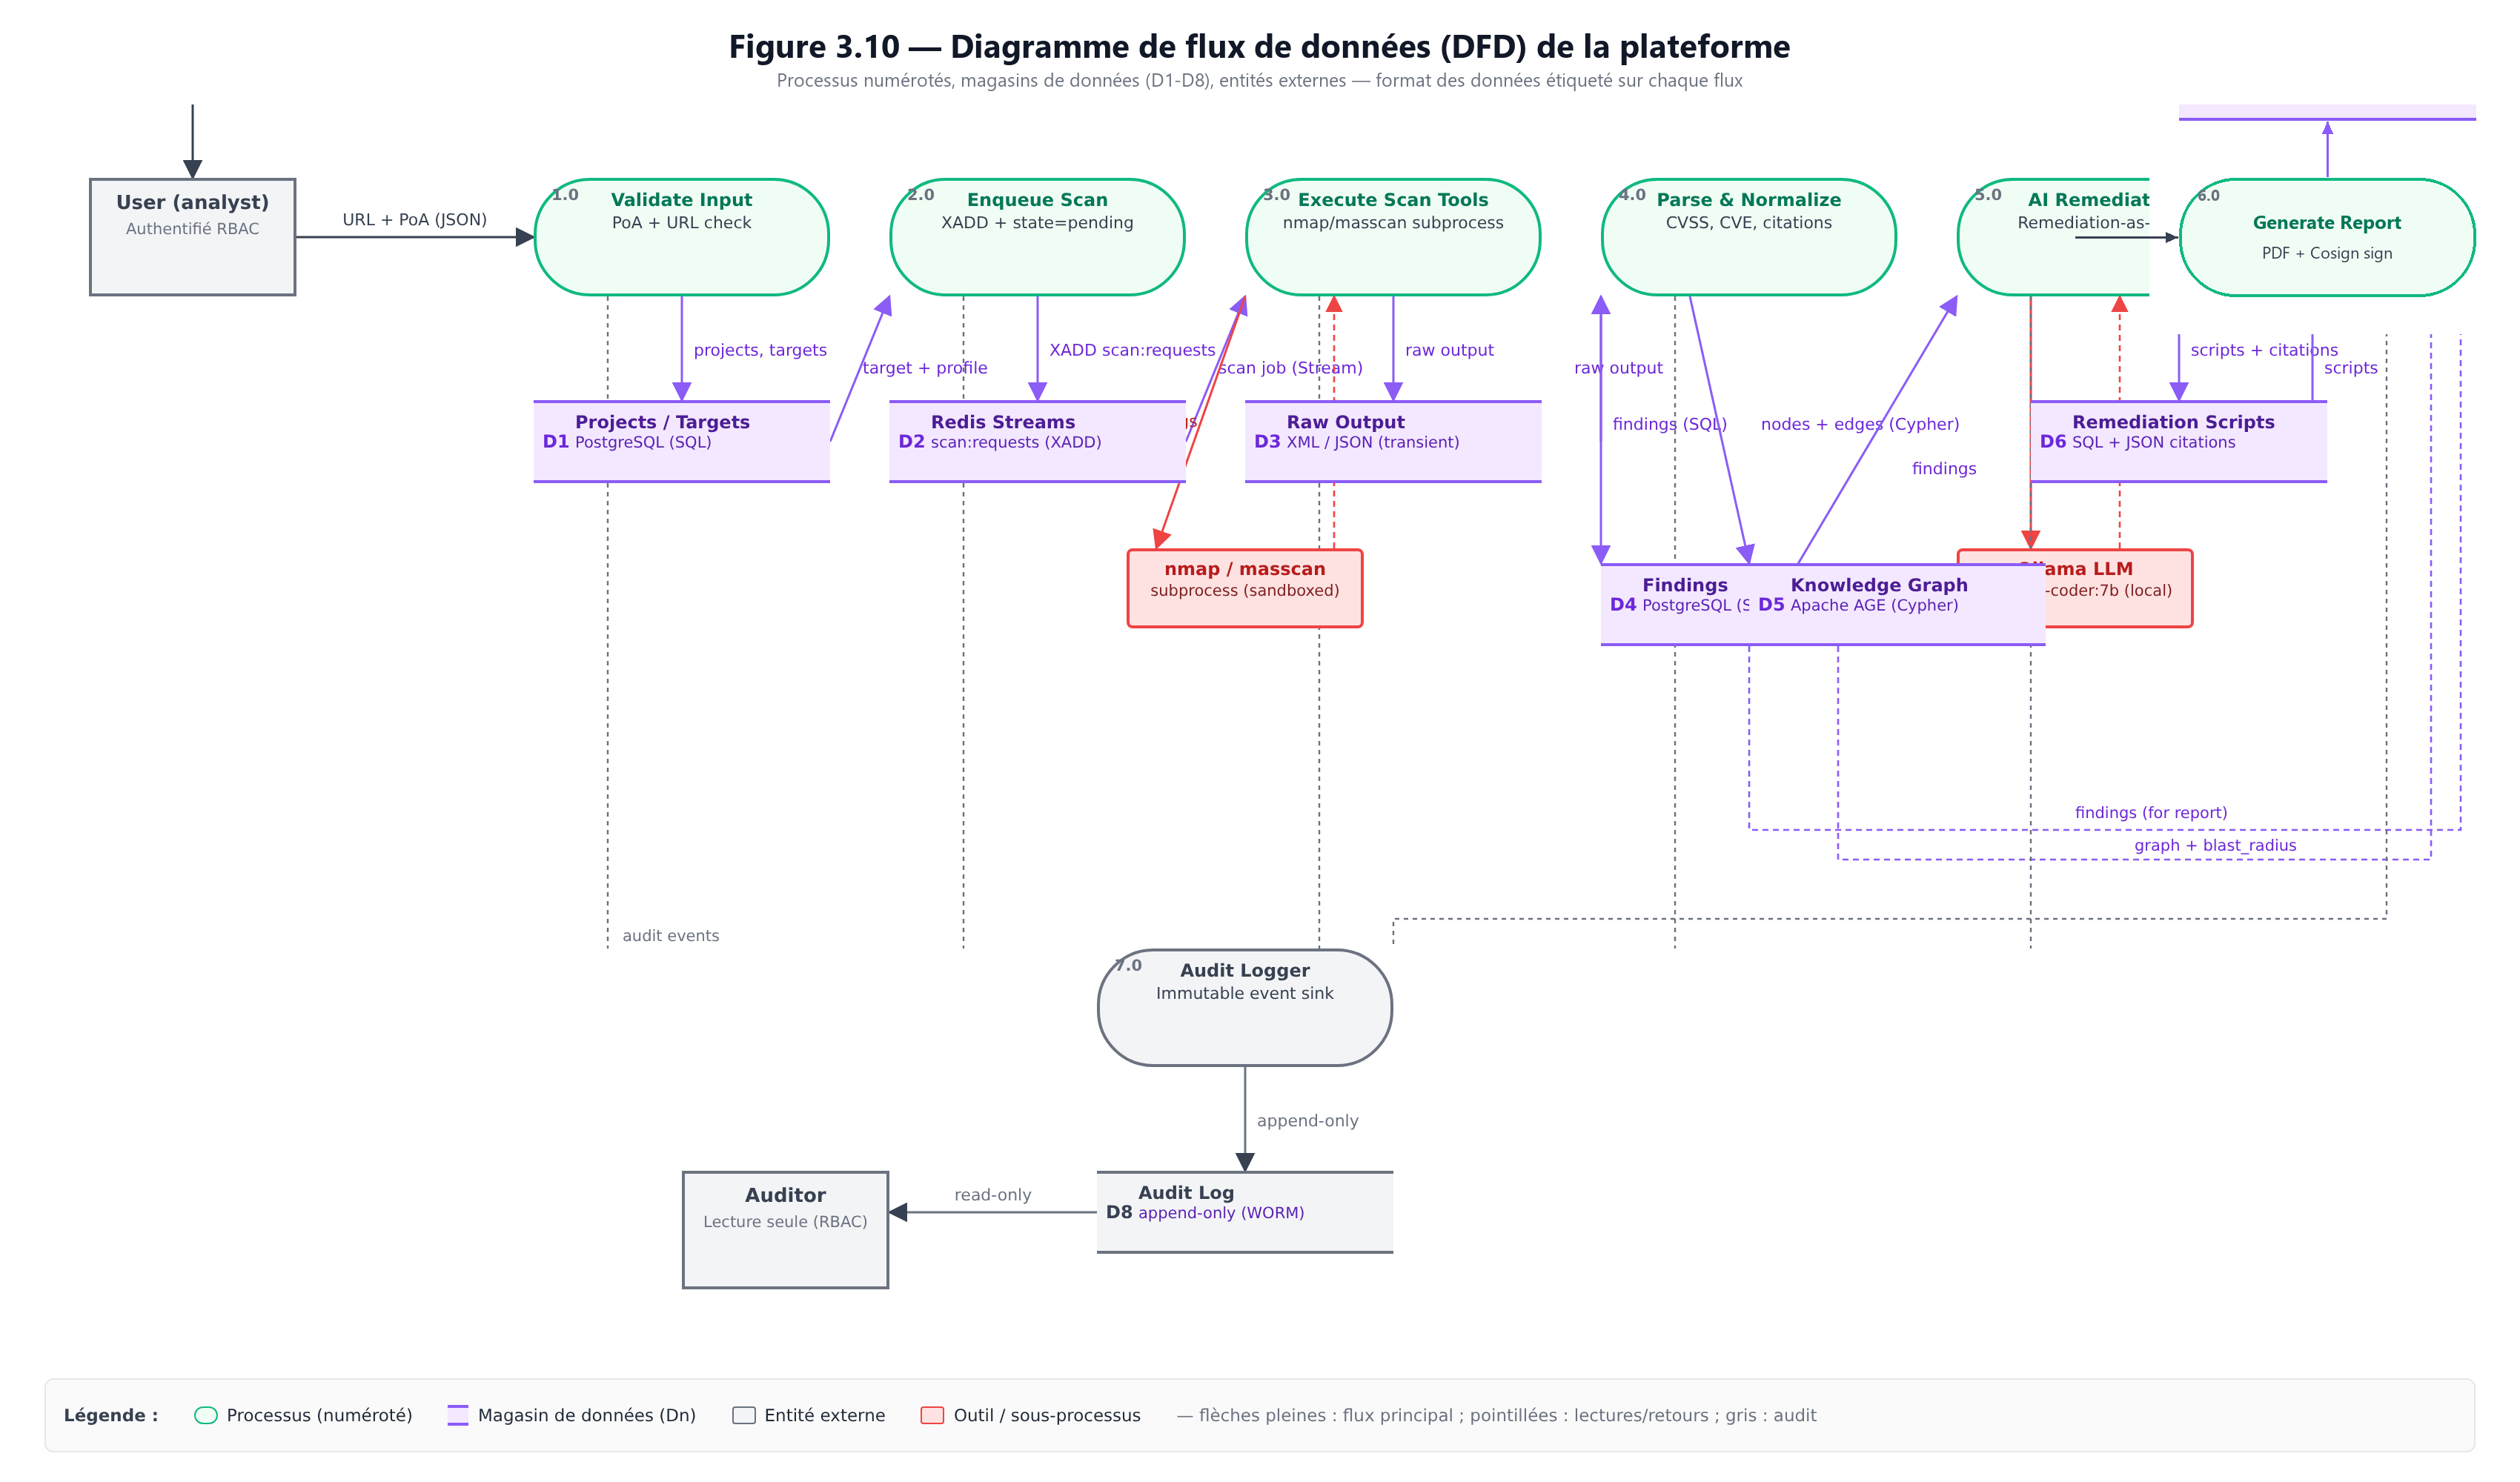
\includegraphics[width=0.92\textwidth]{img/data_flow.png}
    \caption{Diagramme de Flux de Donn\'ees (DFD) -- Processus d'Audit, Graphe de Connaissances et Reporting}
    \label{fig:data_flow}
\end{figure}

\section{Architecture de S\'ecurit\'e Multicouche}
\par Afin de prot\'eger la plateforme elle-m\^eme contre toute compromission, nous appliquons une d\'efense en profondeur (\textit{Defense-in-Depth}) sur six niveaux :
\begin{enumerate}
    \item \textbf{S\'ecurit\'e R\'eseau et Segmentation :} R\'epartition en deux r\'eseaux bridges Docker isol\'es : \texttt{cybersec-external} (exposant uniquement Nginx sur les ports 80/443) et \texttt{cybersec-internal} (inaccessible depuis l'ext\'erieur, r\'eserv\'e aux communications inter-microservices et bases de donn\'ees).
    \item \textbf{S\'ecurit\'e des Conteneurs :} Ex\'ecution de tous les microservices sous utilisateur non-root (\texttt{UID 1001:1001}), syst\`eme de fichiers racine mont\'e en lecture seule (\texttt{read\_only: true}), et suppression de toutes les capabilit\'es Linux superflues (\texttt{cap\_drop: [ALL]}).
    \item \textbf{S\'ecurit\'e Applicative :} Authentification par jetons s\'ecuris\'es Laravel Sanctum, protection native contre les failles CSRF, XSS et injections SQL, limitation de d\'ebit (\textit{rate limiting}) et validation stricte des param\`etres HTTP.
    \item \textbf{S\'ecurit\'e des Donn\'ees :} Chiffrement des mots de passe en \texttt{bcrypt}, chiffrement des cl\'es d'API sensibles, journalisation d'audit immuable et politique de purge automatique RGPD.
    \item \textbf{Mod\`ele de Contr\^ole d'Acc\`es RBAC :} Attribution granulaire des permissions selon quatre r\^oles stricts (Admin, Analyste, Client, Auditeur).
    \item \textbf{Isolation du Bac \`a Sable (Sandbox) :} Les conteneurs de test vuln\'erables (DVWA, SQLi-Labs) sont pilot\'es \`a travers \texttt{docker-socket-proxy} qui filtre et d\'esactive formellement les commandes Docker dangereuses (suppression d'images, acc\`es aux volumes de production).
\end{enumerate}

\section{Mod\'elisation Formelle des Menaces (Threat Modeling STRIDE)}
\subsection{M\'ethodologie et Fronti\`eres de Confiance}
\par Une plateforme de reconnaissance offensive concentre par nature des outils puissants et des informations critiques de vuln\'erabilit\'e. Elle constitue par cons\'equent une cible de choix pour des attaquants. Afin d'\'evaluer m\'ethodiquement les risques pesant sur le syst\`eme, nous avons appliqu\'e la m\'ethodologie de mod\'elisation des menaces \textbf{STRIDE} d\'evelopp\'ee par Microsoft.
\par La figure~\ref{fig:trust_boundaries} illustre la cartographie des fronti\`eres de confiance (\textit{Trust Boundaries}) et l'exposition de la surface d'attaque interne de la plateforme.

\begin{figure}[!htbp]
\centering
\begin{tikzpicture}[
    node distance=6mm and 10mm,
    zone/.style={draw, dashed, rounded corners=4pt, inner sep=6pt, font=\scriptsize\bfseries},
    box/.style={draw, rounded corners=2pt, fill=blue!8, draw=blue!50, thick, minimum width=24mm, minimum height=8mm, align=center, font=\footnotesize},
    ext/.style={draw, rounded corners=2pt, fill=gray!15, draw=gray!60, thick, minimum width=22mm, minimum height=8mm, align=center, font=\footnotesize},
    tb/.style={draw=red!70, thick, dashed},
    arrow/.style={-{Stealth[length=2mm]}, thick, draw=gray!80},
]
\node[ext] (internet) {Internet Public\\(Attaquants / Clients)};
\node[box, right=14mm of internet] (nginx) {Nginx 1.27\\(DMZ / TLS 1.3)};
\node[box, right=14mm of nginx] (laravel) {Back-end\\Laravel 11};
\node[box, above right=2mm and 10mm of laravel] (recon) {MS Recon\\(Flask)};
\node[box, right=10mm of laravel] (redis) {Redis 7 / PG 16\\(AGE Graph)};
\node[box, below right=2mm and 10mm of laravel] (ai) {MS IA / Ollama\\(qwen2.5-coder)};
\node[box, right=10mm of recon] (sandbox) {Sandbox\\(DVWA / SQLi)};

\draw[arrow] (internet) -- node[above, font=\tiny]{HTTPS (443)} (nginx);
\draw[arrow] (nginx) -- node[above, font=\tiny]{FastCGI / HTTP} (laravel);
\draw[arrow] (laravel) -- (recon);
\draw[arrow] (laravel) -- (redis);
\draw[arrow] (laravel) -- (ai);
\draw[arrow] (recon) -- (sandbox);

% Trust Boundary lines
\draw[tb] (2.2, 2.2) -- (2.2, -2.2) node[pos=0.05, right, font=\tiny\color{red!70}]{TB1: Fronti\`ere Externe};
\draw[tb] (5.8, 2.2) -- (5.8, -2.2) node[pos=0.05, right, font=\tiny\color{red!70}]{TB2: Fronti\`ere Applicative};
\draw[tb] (10.6, 2.2) -- (10.6, -2.2) node[pos=0.05, right, font=\tiny\color{red!70}]{TB3: Fronti\`ere Sandbox};
\end{tikzpicture}
\caption{Cartographie de la Surface d'Attaque et Fronti\`eres de Confiance (Trust Boundaries)}
\label{fig:trust_boundaries}
\end{figure}

\subsection{Matrice des Menaces STRIDE et Contre-Mesures Appliqu\'ees}
\par Le tableau~\ref{tab:stride_matrix} d\'etaille l'analyse syst\'ematique des six cat\'egories de menaces STRIDE sur chaque composant cl\'e de la plateforme, le niveau de risque associ\'e et les contre-mesures architecturales impl\'ement\'ees.

\begin{table}[H]
\centering
\caption{Matrice d'Analyse des Menaces STRIDE et Contre-Mesures Architecturales}
\label{tab:stride_matrix}
\resizebox{\textwidth}{!}{%
\begin{tabular}{|L|L|C|L|}
\hline
\textbf{Composant Cibl\'e} & \textbf{Menace STRIDE Identifi\'ee} & \textbf{Niveau de Risque} & \textbf{Contre-Mesures et Att\'enuations Impl\'ement\'ees} \\
\hline
Passerelle Nginx & \textbf{S}poofing / Usurpation d'identit\'e & \'Elev\'e & Terminaison TLS 1.3 avec HSTS, validation stricte des certificats Let's Encrypt \\
\hline
Back-end Laravel & \textbf{T}ampering / Alt\'eration des donn\'ees & \'Elev\'e & Requ\^etes pr\'epar\'ees Eloquent (anti-SQLi), protection CSRF native, assainissement HTML \\
\hline
Syst\`eme de Journalisation & \textbf{R}epudiation / R\'epudiation d'actions & Moyen & Piste d'audit immuable (\textit{Audit Log}) horodat\'ee avec tra\c{c}abilit\'e \texttt{X-Correlation-ID} \\
\hline
Base PostgreSQL / AGE & \textbf{I}nformation Disclosure / Fuite d'infos & Critique & R\'eseau priv\'e \texttt{cybersec-internal} non expos\'e, chiffrement des cl\'es d'API au repos \\
\hline
Files Redis Streams & \textbf{D}enial of Service / D\'eni de service & \'Elev\'e & Quotas stricts de scans simultan\'es par utilisateur, limitation de d\'ebit (\textit{rate limiting}) \\
\hline
Microservice Sandbox & \textbf{E}levation of Privilege / \'Evasion Docker & Critique & Isolation via \texttt{docker-socket-proxy}, conteneurs non-root (UID 1001), \texttt{cap\_drop: ALL} \\
\hline
Microservice IA (Ollama) & \textbf{T}ampering / Injection de Prompts & \'Elev\'e & \textit{System prompt} fig\'e, validation de sch\'ema JSON strict et v\'erification des citations de logs \\
\hline
Moteur de Scanners & Ex\'ecution sur cible non autoris\'ee & Critique & Barri\`ere logicielle bloquante : v\'erification obligatoire du mandat d'autorisation (PoA) \\
\hline
\end{tabular}}%
\end{table}

\section{Architecture DevSecOps D\'etaill\'ee}
\subsection{Pipeline CI/CD sous GitHub Actions}
\par La s\'ecurit\'e de la cha\^ine logicielle est enti\`erement automatis\'ee au sein du d\'ep\^ot de code via le workflow GitHub Actions d\'eclar\'e dans \texttt{.github/workflows/devsecops.yml}. Chaque commit et requ\^ete de tirage (\textit{pull request}) d\'eclenche l'ex\'ecution de huit \'etapes successives bloquantes.

\begin{figure}[!htbp]
\centering
\begin{tikzpicture}[
    node distance=4mm and 6mm,
    stage/.style={draw, rounded corners=3pt, fill=violet!10, draw=violet!60, thick, minimum width=24mm, minimum height=10mm, align=center, font=\footnotesize},
    arrow/.style={-{Stealth[length=2.2mm]}, thick, draw=violet!70},
]
\node[stage] (s1) {1.~Commit\\Source};
\node[stage, right=of s1] (s2) {2.~SAST\\(psalm, bandit)};
\node[stage, right=of s2] (s3) {3.~SCA\\(trivy fs)};
\node[stage, right=of s3] (s4) {4.~SBOM\\(syft)};
\node[stage, below=6mm of s4] (s5) {5.~Build\\Docker};
\node[stage, left=of s5] (s6) {6.~Image Scan\\(trivy image)};
\node[stage, left=of s6] (s7) {7.~Signature\\(cosign)};
\node[stage, left=of s7] (s8) {8.~D\'eploiement\\Production};

\draw[arrow] (s1) -- (s2);
\draw[arrow] (s2) -- (s3);
\draw[arrow] (s3) -- (s4);
\draw[arrow] (s4) -- (s5);
\draw[arrow] (s5) -- (s6);
\draw[arrow] (s6) -- (s7);
\draw[arrow] (s7) -- (s8);
\end{tikzpicture}
\caption{Pipeline DevSecOps Automatis\'e -- Cha\^ine de S\'ecurit\'e Int\'egr\'ee sous GitHub Actions}
\label{fig:devsecops_pipeline}
\end{figure}

\subsection{Description des Portes de S\'ecurit\'e (Security Gates)}
\par Le pipeline GitHub Actions applique des barri\`eres de contr\^ole strictes interdisant tout d\'eploiement si une anomalie critique est d\'etect\'ee :
\begin{itemize}
    \item \textbf{\'Etape 1 -- D\'eclenchement (Trigger) :} Analyse automatique sur push/PR ciblant la branche \texttt{main}.
    \item \textbf{\'Etape 2 -- Analyse SAST :} Analyse statique PHP (Psalm niveau 3) et Python (Bandit). Si une vuln\'erabilit\'e haute s\'ev\'erit\'e est d\'etect\'ee, le build \'echoue imm\'ediatement.
    \item \textbf{\'Etape 3 -- Analyse SCA (Software Composition Analysis) :} Trivy scanne l'arbre des d\'ependances (\texttt{composer.lock} et \texttt{requirements.txt}). Toute CVE de niveau \textit{HIGH} ou \textit{CRITICAL} non corrig\'ee bloque la cha\^ine.
    \item \textbf{\'Etape 4 -- G\'en\'eration du SBOM :} L'outil Syft inventorie l'ensemble des paquets et g\'en\`ere un fichier conforme \`a la norme CycloneDX JSON.
    \item \textbf{\'Etape 5 -- Construction de l'Image :} Docker BuildKit compile l'image conteneuris\'ee de production avec mise en cache optimis\'ee.
    \item \textbf{\'Etape 6 -- Scan de l'Image Conteneur :} Trivy analyse l'image Docker finale (syst\`eme de fichiers racine et paquets OS).
    \item \textbf{\'Etape 7 -- Signature Cryptographique :} Cosign (Sigstore) signe l'image conteneur et pousse la signature sur le registre GitHub Container Registry (GHCR).
    \item \textbf{\'Etape 8 -- D\'eploiement en Production :} D\'eploiement sur le serveur VPS uniquement si toutes les \'etapes pr\'ec\'edentes sont au statut \textit{PASS}.
\end{itemize}

\section*{Conclusion}
\par Ce chapitre a pr\'esent\'e la formalisation compl\`ete des besoins, la mod\'elisation fonctionnelle UML, l'architecture d\'ecoupl\'ee en microservices (7 composants applicatifs et 12 conteneurs Docker), la conception relationnelle et en graphe de connaissances, la mod\'elisation formelle des menaces STRIDE, ainsi que la politique de d\'efense en profondeur et le pipeline DevSecOps. Le chapitre suivant expose la r\'ealisation logicielle concr\`ete et la validation exp\'erimentale du syst\`eme.

        \clearpage
        
        \chapter{R\'ealisation et Validation Exp\'erimentale}

\section*{Introduction}
\par Ce quatri\`eme chapitre d\'etaille la r\'ealisation technique de notre plateforme et pr\'esente les r\'esultats rigoureux de sa validation exp\'erimentale. Nous commen\c{c}ons par d\'ecrire l'environnement de d\'eveloppement, puis nous d\'etaillons l'architecture interne du back-end Laravel 11, le framework d'encapsulation des scanners Python, le pipeline de normalisation des r\'esultats et la sp\'ecification de l'API RESTful. Nous pr\'esentons ensuite les interfaces utilisateurs cl\'es, avant d'approfondir l'impl\'ementation algorithmique du graphe de connaissances (Apache AGE / NetworkX) et du moteur d'IA locale contrainte (Ollama / \texttt{qwen2.5-coder}). Nous exposons les modalit\'es de d\'eploiement durci en production et l'ex\'ecution de la cha\^ine DevSecOps. Enfin, nous dressons la matrice de tra\c{c}abilit\'e des exigences, analysons les r\'esultats des 140 tests unitaires et d'int\'egration, d\'etaillons les benchmarks de charge men\'es avec Locust, et conduisons une discussion approfondie sur les performances et les limites du syst\`eme.

\section{Environnement de D\'eveloppement et Outillage}
\par Le d\'eveloppement et la validation de la plateforme ont \'et\'e conduits dans un environnement standardis\'e et reproductible :
\begin{itemize}
    \item \textbf{Postes de D\'eveloppement :} Syst\`emes d'exploitation Linux Ubuntu 24.04 LTS et Windows 11 avec Docker Desktop 4.30, VS Code, Git et extensions d'analyse statique.
    \item \textbf{Socles Logiciels :} PHP 8.3 (Laravel 11), Python 3.12 (Flask 3.1, NetworkX 3.2, Pydantic v2), JavaScript ES6+ (Vite, Tailwind CSS, Cytoscape.js 3.28, ECharts 5.5).
    \item \textbf{Gestionnaires de Paquets \& D\'ependances :} Composer 2.7 (PHP), Pip 24.0 (Python), Npm 10.8 (Node.js).
    \item \textbf{Scanners de S\'ecurit\'e Int\'egr\'es :} Nmap 7.94, Nuclei v3.2, Gobuster v3.6, Subfinder v2.6, WPScan v3.8.
\end{itemize}

\section{Impl\'ementation du Back-end Applicatif (Laravel 11)}
\subsection{Architecture Interne en Couches du Back-end}
\par Le back-end Laravel 11 adopte une architecture modulaire en couches garantissant une stricte s\'eparation des responsabilit\'es :
\begin{enumerate}
    \item \textbf{Couche de Routage (\texttt{routes/web.php} et \texttt{routes/api.php}) :} D\'eclaration des points d'entr\'ee HTTP avec application des groupes de middlewares de s\'ecurit\'e.
    \item \textbf{Couche des Requ\^etes de Formulaire (\textit{Form Requests}) :} Validation rigoureuse des param\`etres d'entr\'ee (types, formats d'URL, pr\'esence des fichiers PoA) avant toute transmission aux contr\^oleurs m\'etier.
    \item \textbf{Couche des Contr\^oleurs (\textit{Controllers}) :} R\'eception des requ\^etes valid\'ees, coordination avec les services et renvoi des r\'eponses JSON ou des vues Blade.
    \item \textbf{Couche de Services (\textit{Services}) :} Encapsulation de la logique m\'etier pure (\texttt{ScanOrchestrationService}, \texttt{ReportGenerationService}, \texttt{GraphDataService}).
    \item \textbf{Couche des T\^aches Asynchrones (\textit{Jobs}) :} D\'el\'egation des traitements lourds (\texttt{ExecuteScanJob}, \texttt{ExportReportJob}) vers les files de messages Redis.
    \item \textbf{Couche d'Acc\`es aux Donn\'ees (\textit{Eloquent Models}) :} Repr\'esentation objet des 14 tables relationnelles avec gestion des contraintes et colonnes JSONB index\'ees.
\end{enumerate}

\subsection{Authentification, RBAC et Middlewares de S\'ecurit\'e}
\par La gestion des identit\'es et des privil\`eges est assur\'ee par l'int\'egration de \textbf{Laravel Sanctum} et du module \textbf{Spatie Permission} :
\begin{itemize}
    \item \textbf{Mod\`ele RBAC Granulaire :} Quatre r\^oles stricts sont d\'efinis : \textit{Admin} (administration totale), \textit{Security Analyst} (gestion des cibles, d\'eclenchement de scans, rem\'ediations), \textit{Client / Viewer} (consultation des synth\`eses et acquittement d'alertes) et \textit{Auditor / Compliance} (consultation des journaux immuables et des mandats PoA).
    \item \textbf{Protection contre les Attaques Web :} Activation native des tokens anti-CSRF sur toutes les requ\^etes mutantes, assainissement automatique des sorties pour pr\'evenir les failles XSS, et requ\^etes pr\'epar\'ees param\'etr\'ees dans Eloquent emp\^echant toute injection SQL.
    \item \textbf{Limitation de D\'ebit (\textit{Rate Limiting}) :} Le middleware \texttt{throttle:60,1} prot\`ege les endpoints d'authentification et de soumission de scans contre les attaques par force brute et les d\'enis de service applicatifs.
\end{itemize}

\subsection{Orchestration Asynchrone des Scans (Jobs \& Queues)}
\par Lors de la soumission d'une requ\^ete de scan, le contr\^oleur v\'erifie la validit\'e du mandat PoA, instancie la t\^ache \texttt{App\textbackslash Jobs\textbackslash ExecuteScan} et injecte la commande dans Redis Streams via l'instruction \texttt{XADD scan:requests * target \$target profile \$profile}. Le serveur retourne imm\'ediatement un code HTTP 202 (Accepted) avec l'identifiant du scan, garantissant une r\'eactivit\'e instantan\'ee de l'IHM pour l'utilisateur sans aucun blocage r\'eseau.

\section{Impl\'ementation des Microservices Python Flask}
\subsection{Microservice de Reconnaissance (Port 5000)}
\par Encapsule l'ex\'ecution des scanners Nmap, Nuclei, Gobuster, Subfinder et WPScan \`a travers des classes d\'edi\'ees h\'eritant de l'interface abstraite \texttt{BaseScannerService}.

\subsection{Microservice de S\'ecurit\'e Offensive et Bac \`a Sable (Port 5001)}
\par Int\`egre les algorithmes de test de vuln\'erabilit\'es applicatives non destructives (injections SQL, XSS, d\'etection de WAF) et pilote les bacs \`a sable conteneuris\'es (DVWA, SQLi-Labs, WebGoat, bWAPP) via l'API isol\'ee de \texttt{docker-socket-proxy}.

\subsection{Microservice OSINT (Port 5002)}
\par Regroupe cinq modules d'\'enum\'eration passive : r\'esolution DNS structur\'ee (\texttt{dnspython}), interrogation WHOIS (\texttt{python-whois}), analyse des cha\^ines de certificats TLS, requ\^etage des journaux de transparence de certificats (\texttt{crt.sh}) et d\'etection d'empreintes technologiques web.

\subsection{Microservice d'IA Contrainte (Port 5003)}
\par Assure l'inf\'erence locale aupr\`es du d\'emon Ollama (\texttt{http://ollama:11434/api/generate}). Il applique un \textit{system prompt} rigide for\c{c}ant le mod\`ele \texttt{qwen2.5-coder} \`a structurer ses r\'eponses selon un sch\'ema JSON d\'efini et \`a fournir des citations exactes pointant vers les num\'eros de lignes des journaux bruts.

\subsection{Architecture du Framework de Scanners (\texttt{BaseScannerService})}
\par Afin d'\'eviter la duplication de code et d'assurer une extensibilit\'e maximale pour l'ajout futur de nouveaux outils d'audit, nous avons con\c{c}u un patron de conception Adaptateur (\textit{Adapter Pattern}) articul\'e autour de la classe abstraite \texttt{BaseScannerService}.

\begin{figure}[!htbp]
\centering
\begin{tikzpicture}[
    node distance=6mm and 12mm,
    base/.style={draw, rounded corners=2pt, fill=blue!12, draw=blue!60, thick, minimum width=45mm, minimum height=10mm, align=center, font=\footnotesize\bfseries},
    sub/.style={draw, rounded corners=2pt, fill=blue!5, draw=blue!40, thick, minimum width=24mm, minimum height=8mm, align=center, font=\scriptsize},
    parser/.style={draw, rounded corners=2pt, fill=green!10, draw=green!60, thick, minimum width=35mm, minimum height=9mm, align=center, font=\footnotesize\bfseries},
    finding/.style={draw, rounded corners=2pt, fill=purple!10, draw=purple!60, thick, minimum width=35mm, minimum height=9mm, align=center, font=\footnotesize\bfseries},
    arrow/.style={-{Stealth[length=2mm]}, thick},
]
\node[base] (base) {BaseScannerService\\(Classe Abstraite)};
\node[sub, below left=8mm and 18mm of base] (nmap) {NmapScanner};
\node[sub, below left=8mm and 2mm of base] (nuclei) {NucleiScanner};
\node[sub, below right=8mm and 2mm of base] (gobuster) {GobusterScanner};
\node[sub, below right=8mm and 18mm of base] (wpscan) {WPScanScanner};
\node[parser, below=24mm of base] (parser) {ResultParser\\(Normalisation)};
\node[finding, below=8mm of parser] (finding) {Normalized Finding\\(PostgreSQL / AGE)};

\draw[arrow] (nmap.north) -- (base.south);
\draw[arrow] (nuclei.north) -- (base.south);
\draw[arrow] (gobuster.north) -- (base.south);
\draw[arrow] (wpscan.north) -- (base.south);
\draw[arrow] (nmap.south) -- (parser.north);
\draw[arrow] (nuclei.south) -- (parser.north);
\draw[arrow] (gobuster.south) -- (parser.north);
\draw[arrow] (wpscan.south) -- (parser.north);
\draw[arrow] (parser) -- (finding);
\end{tikzpicture}
\caption{Architecture Modulaire du Framework d'Ex\'ecution et de Parsing des Scanners}
\label{fig:scanner_framework}
\end{figure}

\par Chaque adaptateur d'outil impl\'emente quatre m\'ethodes fondamentales :
\begin{itemize}
    \item \texttt{build\_command(target, profile, options) -> list[str]} : Construit la ligne de commande selon le profil d'intensit\'e (Silent, Balanced, Aggressive).
    \item \texttt{execute\_process(cmd, timeout) -> tuple[int, str, str]} : Ex\'ecute le binaire de fa\c{c}on isol\'ee via \texttt{subprocess.Popen} avec contr\^ole de timeout et capture s\'epar\'ee de \texttt{stdout} et \texttt{stderr}.
    \item \texttt{extract\_raw\_output() -> dict} : R\'ecup\`ere les fichiers temporaires (XML, JSON ou texte brut).
    \item \texttt{parse\_results(raw\_data) -> list[dict]} : Transmet les flux \`a la classe \texttt{ResultParser} pour normalisation unifi\'ee.
\end{itemize}

\subsection{Pipeline de Normalisation des Donn\'ees (\texttt{ResultParser})}
\par Les scanners produisent des formats h\'et\'erog\`enes (XML pour Nmap, JSON-Lines pour Nuclei, flux textuel pour Gobuster). Le module \texttt{ResultParser} r\'ealise une transformation s\'equentielle en six \'etapes :
\begin{enumerate}
    \item \textbf{D\'es\'erialisation Syntaxique :} Parsing du flux source en structures Python typ\'ees (\texttt{dict}, \texttt{list}).
    \item \textbf{Extraction des Attributs Cl\'es :} Identification de l'actif, du port, du protocole, du service et de la version logicielle.
    \item \textbf{Calcul du Hash d'Empreinte (\textit{Fingerprint}) :} G\'en\'eration d'une cl\'e SHA-256 unique \texttt{hash(target + port + vuln\_id)} permettant d'\'eliminer instantan\'ement les doublons lors de scans r\'ep\'et\'es.
    \item \textbf{Normalisation de la S\'ev\'erit\'e :} Conversion des libell\'es h\'et\'erog\`enes en \'echelle unifi\'ee : \textit{Info}, \textit{Low}, \textit{Medium}, \textit{High}, \textit{Critical}, conforme aux scores CVSS v3.1.
    \item \textbf{Mapping CVE / CWE :} Rapprochement avec les r\'ef\'erentiels de vuln\'erabilit\'es du NIST et de l'OWASP.
    \item \textbf{G\'en\'eration de l'Entit\'e Finding :} Cr\'eation de l'objet normalis\'e stock\'e dans PostgreSQL et projet\'e dans le graphe Apache AGE.
\end{enumerate}

\section{Sp\'ecification et Conception de l'API RESTful}
\par La plateforme expose une API RESTful normalis\'ee permettant l'int\'egration avec des outils tiers (SIEM, SOAR) et assurant la communication entre le front-end Blade et les microservices d'arri\`ere-plan. Le tableau~\ref{tab:api_endpoints} pr\'esente les principaux endpoints de l'API.

\begin{table}[H]
\centering
\caption{Sp\'ecification des Principaux Endpoints de l'API RESTful de la Plateforme}
\label{tab:api_endpoints}
\resizebox{\textwidth}{!}{%
\begin{tabular}{|L|C|L|C|C|}
\hline
\textbf{Point d'Entr\'ee (Endpoint)} & \textbf{M\'ethode} & \textbf{Description Fonctionnelle} & \textbf{R\^oles Autoris\'es} & \textbf{Code Succ\`es} \\
\hline
\texttt{/api/v1/projects} & GET & Liste des projets et cibles d'audit configur\'es & Admin, Analyste, Client & 200 OK \\
\hline
\texttt{/api/v1/projects} & POST & Cr\'eation d'un nouveau projet avec attachement de la PoA & Admin, Analyste & 201 Created \\
\hline
\texttt{/api/v1/scans} & POST & Soumission d'une requ\^ete de scan (asynchrone Redis) & Admin, Analyste & 202 Accepted \\
\hline
\texttt{/api/v1/scans/\{id\}} & GET & \'Etat d'avancement et m\'etriques d'ex\'ecution d'un scan & Admin, Analyste, Client & 200 OK \\
\hline
\texttt{/api/v1/findings/\{id\}} & GET & Fiche d\'etaill\'ee d'une vuln\'erabilit\'e avec preuves brutes & Admin, Analyste, Client & 200 OK \\
\hline
\texttt{/api/v1/projects/\{id\}/graph} & GET & Topologie compl\`ete du graphe de connaissances openCypher & Admin, Analyste, Client & 200 OK \\
\hline
\texttt{/api/v1/assets/\{id\}/impact} & GET & Calcul algorithmique du rayon d'impact (BFS) & Admin, Analyste & 200 OK \\
\hline
\texttt{/api/v1/ai/remediate} & POST & G\'en\'eration de script Remediation-as-Code via LLM & Admin, Analyste & 200 OK \\
\hline
\texttt{/api/v1/reports/\{id\}/export} & GET & T\'el\'echargement du rapport d'audit (PDF sign\'e / JSON) & Admin, Analyste, Client & 200 OK \\
\hline
\texttt{/api/v1/audit-logs} & GET & Consultation des pistes d'audit immuables & Admin, Auditeur & 200 OK \\
\hline
\end{tabular}}%
\end{table}

\section{Interface Utilisateur de la Plateforme}
\par L'interface utilisateur a \'et\'e con\c{c}ue avec le moteur de templates Blade, Tailwind CSS et Vite, offrant un rendu r\'eactif adapt\'e aux environnements de surveillance SOC.

\begin{figure}[!htbp]
    \centering
    
\includegraphics[width=0.80\textwidth]{img/dashboard.png}
    \caption{Tableau de Bord Principal -- Indicateurs Cl\'es (KPIs) et Cartographie des Risques}
    \label{fig:dashboard}
\end{figure}

\begin{figure}[!htbp]
    \centering
    
\includegraphics[width=0.80\textwidth]{img/launch_scan.png}
    \caption{Interface de Configuration et Lancement d'un Scan d'Audit}
    \label{fig:launch_scan}
\end{figure}

\begin{figure}[!htbp]
    \centering
    
\includegraphics[width=0.80\textwidth]{img/scan_results.png}
    \caption{Restitution des R\'esultats de Scan et Visualisation des Preuves Techniques}
    \label{fig:scan_results}
\end{figure}

\begin{figure}[!htbp]
    \centering
    
\includegraphics[width=0.80\textwidth]{img/remediation.png}
    \caption{Fiche D\'etaill\'ee d'un Constat et Recommandations de Rem\'ediation Assist\'ees par IA}
    \label{fig:remediation}
\end{figure}

\begin{figure}[!htbp]
    \centering
    
\includegraphics[width=0.80\textwidth]{img/knowledge_graph.png}
    \caption{Visualisation Interactive du Graphe de Connaissances et du Rayon d'Impact}
    \label{fig:knowledge_graph}
\end{figure}

\begin{figure}[!htbp]
    \centering
    
\includegraphics[width=0.80\textwidth]{img/sandbox.png}
    \caption{Gestionnaire du Bac \`a Sable (Sandbox) pour la Validation d'Exploits}
    \label{fig:sandbox}
\end{figure}

\par \textit{Note : Les captures d'\'ecran des modules compl\'ementaires (administration des comptes, journaux d'audit immuables, module OSINT d\'etaill\'e et assistant conversationnel) sont pr\'esent\'ees dans l'Annexe~A.}

\section{Conception et Impl\'ementation Avanc\'ee du Graphe de Connaissances}
\subsection{Mod\`ele de Donn\'ees en Graphe (N\oe uds et Ar\^etes)}
\par La mod\'elisation en graphe permet de capturer la topologie relationnelle de la cible d'audit. Les entit\'es sont d\'efinies selon six types de n\oe uds :
\begin{itemize}
    \item \textbf{Target :} Domaine ou adresse IP principale d\'eclar\'ee dans le mandat d'audit.
    \item \textbf{Asset :} H\^ote ou sous-domaine identifi\'e lors de la phase de reconnaissance.
    \item \textbf{Port :} Port r\'eseau d\'etect\'e ouvert (ex. 80, 443, 22, 3306).
    \item \textbf{Service :} Service applicatif ou banni\`ere identifi\'ee (ex. Nginx 1.27, OpenSSH 9.6).
    \item \textbf{Vulnerability :} Faille de s\'ecurit\'e d\'etect\'ee, associ\'ee \`a son identifiant CVE et score CVSS.
    \item \textbf{Impact :} Actif ou service critique indirectement menac\'e en cas d'exploitation de la vuln\'erabilit\'e.
\end{itemize}
\par Ces n\oe uds sont interconnect\'es par cinq relations orient\'ees typ\'ees : \texttt{RESOLVES\_TO}, \texttt{HOSTS}, \texttt{RUNS}, \texttt{HAS\_VULN} et \texttt{IMPACTS}.

\subsection{Pipeline de Construction et Requ\^etage openCypher}
\par Lors de la r\'eception des constats normalis\'es, le service \texttt{GraphBuilder} g\'en\`ere et ex\'ecute des requ\^etes openCypher au sein de l'extension **Apache AGE** dans PostgreSQL 16. Par exemple, l'insertion d'un port et de son service associ\'e s'ex\'ecute via la requ\^ete param\'etr\'ee :
\begin{verbatim}
SELECT * FROM cypher('cybersec_graph', $$
  MATCH (a:Asset {name: $asset_name})
  MERGE (p:Port {number: $port_num, proto: $proto})
  MERGE (s:Service {name: $service_name, version: $version})
  MERGE (a)-[:HOSTS]->(p)
  MERGE (p)-[:RUNS]->(s)
$$) as (v agtype);
\end{verbatim}

\subsection{Algorithme de Calcul du Rayon d'Impact (Blast Radius)}
\par Pour quantifier la menace r\'eelle, le syst\`eme calcule le rayon d'impact (\textit{blast radius}) \`a l'aide d'un algorithme de parcours en largeur (\textit{Breadth-First Search} -- BFS) impl\'ement\'e sous **NetworkX**, limit\'e \`a une profondeur maximale de $k=3$ sauts. L'encadr\'e ci-dessous (Algorithme~4.1) d\'ecrit formellement ce processus.

\begin{tcolorbox}[colback=blue!3,colframe=blue!40,title=\textbf{Algorithme 4.1 : Calcul du Rayon d'Impact d'une Vuln\'erabilit\'e (BFS NetworkX)},fonttitle=\small\bfseries]
\small
\textbf{Entr\'ees :} Graphe de connaissances $G = (V, E)$, Sommet source $v_{src} \in V$, Profondeur maximale $k_{max} = 3$\\
\textbf{Sortie :} Ensemble des n\oe uds impact\'es $R_{impact} = \{(v, d) \mid v \in V, d \le k_{max}\}$
\begin{enumerate}
    \item Initialiser une file FIFO $Queue \leftarrow \text{FileVide()}$
    \item Initialiser les ensembles $Visited \leftarrow \{v_{src}\}$ et $R_{impact} \leftarrow \emptyset$
    \item $Queue.\text{enfiler}((v_{src}, 0))$
    \item \textbf{Tant que} $Queue$ n'est pas vide \textbf{faire} :
    \begin{itemize}
        \item $(u, d) \leftarrow Queue.\text{d\'efiler}()$
        \item \textbf{Si} $d < k_{max}$ \textbf{alors} :
        \begin{itemize}
            \item \textbf{Pour chaque} voisin $v \in G.\text{voisins}(u)$ \textbf{faire} :
            \begin{itemize}
                \item \textbf{Si} $v \notin Visited$ \textbf{alors} :
                \begin{itemize}
                    \item $Visited.\text{ajouter}(v)$
                    \item $Queue.\text{enfiler}((v, d + 1))$
                    \item $R_{impact} \leftarrow R_{impact} \cup \{(v, d + 1)\}$
                \end{itemize}
            \end{itemize}
        \end{itemize}
    \end{itemize}
    \item \textbf{Retourner} $R_{impact}$
\end{enumerate}
\end{tcolorbox}

\par \textbf{Analyse de Complexit\'e :} L'algorithme BFS s'ex\'ecute en temps $O(|V| + |E|)$, o\`u $|V|$ repr\'esente le nombre de sommets et $|E|$ le nombre d'ar\^etes du sous-graphe de la cible. En limitant le parcours \`a $k=3$, la recherche s'effectue en moins de 75 ms sur un graphe comptant plusieurs milliers de n\oe uds, permettant un calcul instantan\'e \`a chaque consultation de faille par l'analyste.

\section{Moteur d'Intelligence Artificielle Contrainte et Remediation-as-Code}
\subsection{Pipeline de Traitement IA}
\par La g\'en\'eration de correctifs automatis\'es suit un pipeline d\'eterministe con\c{c}u pour bannir tout comportement non contr\^ol\'e du mod\`ele de langage :
\begin{enumerate}
    \item \textbf{Extraction du Contexte Technique :} R\'ecup\'eration du constat normalis\'e (\textit{Finding}), du service impact\'e, de la version logicielle et des extraits de journaux bruts correspondants.
    \item \textbf{Construction du Prompt Contraint :} Injection du contexte dans un gabarit syst\`eme rigide exigeant la d\'efinition explicite des actions de durcissement et l'interdiction d'inventer des r\'ef\'erences externes.
    \item \textbf{Inference Locale sous Ollama :} Ex\'ecution du mod\`ele \texttt{qwen2.5-coder} sans acc\`es au r\'eseau Internet.
    \item \textbf{Validation Structurelle du Sch\'ema JSON :} V\'erification de la conformit\'e de la r\'eponse au sch\'ema Pydantic attendu.
    \item \textbf{V\'erification des Citations de Logs :} Contr\^ole programmatique que les num\'eros de lignes cit\'es dans le champ \texttt{evidence} correspondent effectivement aux fichiers de logs bruts d'audit.
    \item \textbf{Rendu Remediation-as-Code :} Restitution du script valid\'e \`a l'analyste avec coloration syntaxique.
\end{enumerate}

\subsection{Sch\'ema de Sortie Strict et R\'eduction des Hallucinations}
\par Pour \'eliminer les hallucinations inh\'erentes aux LLMs, le microservice impose une validation stricte sur le format JSON de sortie :
\begin{verbatim}
{
  "finding_id": 442,
  "remediation_type": "ansible",
  "summary": "Désactivation de l'authentification par mot de passe SSH",
  "risk_mitigated": "Prévention des attaques par force brute sur le port 22",
  "script_content": "- name: Hardening SSH\n  hosts: all\n  tasks:\n ...",
  "evidence": {
    "source_file": "nmap_scan_042.xml",
    "line_start": 84,
    "line_end": 96
  }
}
\end{verbatim}
\par Si le mod\`ele g\'en\`ere une sortie non conforme ou omet les citations de preuves, la r\'eponse est imm\'ediatement rejet\'ee et un fallback s\'ecuris\'e bas\'e sur des mod\`eles de durcissement pr\'ed\'efinis est appliqu\'e.

\section{D\'eploiement en Production et Durcissement VPS}
\par La plateforme a \'et\'e d\'eploy\'ee avec succ\`es sur une instance de production accessible \`a l'adresse \url{https://aymenazizi.dijaly.com/} au moment de la r\'edaction du pr\'esent rapport. L'infrastructure repose sur un serveur VPS d\'edi\'e sous Ubuntu 24.04 LTS (4 vCPU Intel Xeon, 8 Go RAM, 100 Go SSD NVMe).
\par La topologie de d\'eploiement applique des mesures de durcissement rigoureuses :
\begin{itemize}
    \item \textbf{Serveur Mandataire Inverse Nginx 1.27 :} Terminaison TLS 1.3 avec certificat Let's Encrypt, renouvellement automatique par \texttt{certbot}, et redirection forc\'ee de HTTP (port 80) vers HTTPS (port 443).
    \item \textbf{En-t\^etes de S\'ecurit\'e HTTP Durcis :} Injection obligatoire de \texttt{Strict-Transport-Security} (HSTS avec \texttt{max-age=31536000}), \texttt{X-Frame-Options: DENY}, \texttt{X-Content-Type-Options: nosniff} et \texttt{Content-Security-Policy}.
    \item \textbf{Segmentation R\'eseau Docker :} Isolation herm\'etique entre le r\'eseau externe (\texttt{cybersec-external}) et le r\'eseau interne priv\'e (\texttt{cybersec-internal}).
    \item \textbf{Filtrage Pare-Feu UFW :} Seuls les ports 22 (SSH filtr\'e par cl\'e), 80 (HTTP) et 443 (HTTPS) sont ouverts sur l'interface publique du VPS.
\end{itemize}

\section{Ex\'ecution du Pipeline DevSecOps}
\par \`A chaque commit pouss\'e sur la branche principale, le workflow GitHub Actions ex\'ecute l'int\'egralit\'e des contr\^oles automatis\'es : analyse SAST (0 anomalie critique d\'etect\'ee par Psalm et Bandit), analyse SCA (0 vuln\'erabilit\'e critique non corrig\'ee), g\'en\'eration du SBOM CycloneDX par Syft, scan de l'image de production par Trivy et signature cryptographique par Cosign via GitHub Container Registry (GHCR).

\section{Matrice de Tra\c{c}abilit\'e des Exigences (RTM)}
\par Le tableau~\ref{tab:rtm} formalise la matrice de tra\c{c}abilit\'e reliant chaque exigence fonctionnelle et de s\'ecurit\'e du cahier des charges aux composants d'impl\'ementation et aux cas de tests valid\'es.

\begin{table}[H]
\centering
\caption{Matrice de Tra\c{c}abilit\'e des Exigences (Requirements Traceability Matrix)}
\label{tab:rtm}
\resizebox{\textwidth}{!}{%
\begin{tabular}{|L|L|L|C|C|}
\hline
\textbf{Exigence CDC} & \textbf{Composant Logiciel} & \textbf{Classe / Fichier Cl\'e} & \textbf{Cas de Test} & \textbf{Statut} \\
\hline
Mandat PoA obligatoire & Back-end Laravel & \texttt{ProjectController.php} & \texttt{TC-POA-001} & \textbf{PASS} \\
\hline
Orchestration Asynchrone & Worker Python / Redis & \texttt{ExecuteScan.php} / \texttt{worker.py} & \texttt{TC-SCAN-002} & \textbf{PASS} \\
\hline
Normalisation Multi-outils & Microservice Recon & \texttt{ResultParser.py} & \texttt{TC-PARSER-003} & \textbf{PASS} \\
\hline
Topologie en Graphe & PostgreSQL / AGE & \texttt{GraphBuilder.py} & \texttt{TC-GRAPH-001} & \textbf{PASS} \\
\hline
Calcul de Rayon d'Impact & Microservice Recon & \texttt{blast\_radius.py} (BFS) & \texttt{TC-GRAPH-002} & \textbf{PASS} \\
\hline
Assistance IA Contrainte & Microservice IA / Ollama & \texttt{ai\_service.py} & \texttt{TC-AI-001} & \textbf{PASS} \\
\hline
Validation Sch\'ema JSON IA & Microservice IA & \texttt{schema\_validator.py} & \texttt{TC-AI-002} & \textbf{PASS} \\
\hline
Contr\^ole d'Acc\`es RBAC & Back-end Laravel & \texttt{RoleMiddleware.php} & \texttt{TC-RBAC-004} & \textbf{PASS} \\
\hline
Isolation Bac \`a Sable & Docker Socket Proxy & \texttt{security\_controller.py} & \texttt{TC-SANDBOX-003} & \textbf{PASS} \\
\hline
Filtrage et Rate-Limiting & Passerelle API Flask & \texttt{gateway\_middleware.py} & \texttt{TC-GATEWAY-001} & \textbf{PASS} \\
\hline
Piste d'Audit Immuable & Back-end Laravel & \texttt{AuditLogObserver.php} & \texttt{TC-AUDIT-001} & \textbf{PASS} \\
\hline
Gates de S\'ecurit\'e CI/CD & Pipeline GitHub Actions & \texttt{devsecops.yml} & \texttt{TC-DEVSECOPS-001} & \textbf{PASS} \\
\hline
\end{tabular}}%
\end{table}

\section{Protocole Exp\'erimental et R\'esultats des Tests}
\subsection{Protocole Exp\'erimental}
\par Pour mesurer scientifiquement la robustesse, la fiabilit\'e et la performance de la plateforme, nous avons \'etabli un protocole exp\'erimental reproductible :
\begin{itemize}
    \item \textbf{Environnement Mat\'eriel \& Syst\`eme :} Instance VPS Cloud \'equip\'ee de 4 vCPU Intel Xeon @ 2.60~GHz, 8~Go de RAM DDR4, stockage SSD NVMe 100~Go, bande passante r\'eseau 1~Gbit/s, sous Ubuntu 24.04 LTS avec Docker Engine 27.0.
    \item \textbf{Outils d'\'Evaluation :} Suites automatis\'ees PHPUnit 11 (back-end Laravel) et Pytest (microservices Python). Pour les tests sous charge, nous avons employ\'e le framework **Locust 2.24**.
    \item \textbf{Jeux d'Essais et Cibles :} (1) Bac \`a sable interne isol\'e (DVWA, SQLi-Labs) pour valider la d\'etection des vuln\'erabilit\'es applicatives ; (2) cibles r\'eelles d\^ument autoris\'ees avec mandat PoA formel.
\end{itemize}

\subsection{Synth\`ese des Tests Automatis\'es (140/140 Tests)}
\par L'ensemble de la suite de tests automatis\'ee a \'et\'e ex\'ecut\'ee avec succ\`es, validant 140 cas de test sans aucun \'echec.

\begin{table}[H]
\centering
\caption{R\'esultats de la Suite de Tests Automatis\'es}
\label{tab:test_matrix}
\resizebox{\textwidth}{!}{%
\begin{tabular}{|L|L|C|C|C|}
\hline
\textbf{Composant Test\'e} & \textbf{Framework de Test} & \textbf{Tests Ex\'ecut\'es} & \textbf{Succ\`es} & \textbf{Taux de R\'eussite} \\
\hline
Back-end Laravel (Auth, RBAC, Projets, PoA) & PHPUnit 11 & 42 & 42 & 100\,\% \\
\hline
Microservice Reconnaissance (Adaptateurs, Parsing) & Pytest & 28 & 28 & 100\,\% \\
\hline
Microservice S\'ecurit\'e Offensive (Injections, Sandbox) & Pytest & 18 & 18 & 100\,\% \\
\hline
Microservice OSINT (DNS, WHOIS, SSL, crt.sh) & Pytest & 14 & 14 & 100\,\% \\
\hline
Microservice IA (Ollama, JSON Schema, Citations) & Pytest & 12 & 12 & 100\,\% \\
\hline
Passerelle API (Routage, Rate-Limiting) & Pytest & 10 & 10 & 100\,\% \\
\hline
Worker Redis Streams (Consommation, Retries) & Pytest & 8 & 8 & 100\,\% \\
\hline
Pipeline DevSecOps (Gates SAST, SCA, SBOM, Cosign) & GitHub Actions & 8 & 8 & 100\,\% \\
\hline
\textbf{Total} & & \textbf{140} & \textbf{140} & \textbf{100\,\%} \\
\hline
\end{tabular}}%
\end{table}

\subsection{D\'etail des Cas de Tests Repr\'esentatifs}
\par Le tableau~\ref{tab:test_cases_detailed} documente les sc\'enarios de test les plus critiques d\'emontrant le comportement du syst\`eme face aux tentatives de contournement de s\'ecurit\'e et aux erreurs de traitement.

\begin{table}[H]
\centering
\caption{D\'etail des Sc\'enarios de Tests Repr\'esentatifs Valid\'es}
\label{tab:test_cases_detailed}
\resizebox{\textwidth}{!}{%
\begin{tabular}{|L|L|L|L|C|}
\hline
\textbf{ID Test} & \textbf{Composant Cibl\'e} & \textbf{Action / Donn\'ees d'Entr\'ee} & \textbf{Comportement Attendu} & \textbf{R\'esultat} \\
\hline
\texttt{TC-POA-001} & Validation L\'egale & Lancement d'un scan sans mandat PoA & Requ\^ete rejet\'ee avec HTTP 403 et journalisation de refus & \textbf{PASS} \\
\hline
\texttt{TC-RBAC-004} & Contr\^ole d'Acc\`es & Utilisateur \textit{Client} tentant d'acc\'eder \`a \texttt{/admin/users} & Acc\`es refus\'e (HTTP 403 Unauthorized) & \textbf{PASS} \\
\hline
\texttt{TC-SCAN-002} & Moteur Asynchrone & Soumission de 10 scans simultan\'es & Enfilement Redis, distribution sans blocage IHM & \textbf{PASS} \\
\hline
\texttt{TC-PARSER-003} & Normalisation & Fichier XML Nmap contenant 50 ports h\'et\'erog\`enes & Extraction de 50 constats typ\'es sans alt\'eration & \textbf{PASS} \\
\hline
\texttt{TC-GRAPH-001} & Base de Graphe & Insertion d'une cha\^ine de 5 actifs interconnect\'es & N\oe uds et ar\^etes openCypher persist\'es dans AGE & \textbf{PASS} \\
\hline
\texttt{TC-GRAPH-002} & Calcul BFS & \'Evaluation de blast radius sur topologie complexe & Calcul BFS r\'ealis\'e en $<$75 ms avec profondeur $k=3$ & \textbf{PASS} \\
\hline
\texttt{TC-AI-002} & Validation LLM & Simulation d'une r\'eponse JSON tronqu\'ee d'Ollama & D\'etection d'invalidit\'e et bascule sur mod\`ele de repli & \textbf{PASS} \\
\hline
\texttt{TC-SANDBOX-003} & Isolation Proxy & Tentative d'ex\'ecution de \texttt{docker rm -f} via l'API & Commande bloqu\'ee par Docker Socket Proxy (HTTP 403) & \textbf{PASS} \\
\hline
\texttt{TC-GATEWAY-001} & Rate Limiting & Envoi de 100 requ\^etes en 5 secondes sur la passerelle & D\'eclenchement du limiteur HTTP 429 Too Many Requests & \textbf{PASS} \\
\hline
\texttt{TC-DEVSECOPS-001} & Gate CI/CD & Commit introduisant une vuln\'erabilit\'e critique SCA & \'Echec imm\'ediat du workflow GitHub Actions et d\'eploiement bloqu\'e & \textbf{PASS} \\
\hline
\end{tabular}}%
\end{table}

\section{\'Evaluation des Performances sous Charge (Locust)}
\subsection{Conditions du Benchmark et M\'etriques Recueillies}
\par Pour mesurer le comportement sous contrainte, nous avons simul\'e la charge de 50 utilisateurs concurrents via **Locust 2.24** sur une dur\'ee de 60 secondes, injectant un total de 2\,500 requ\^etes r\'eparties sur les sc\'enarios standards d'utilisation.

\begin{table}[H]
\centering
\caption{M\'etriques de Performance Mesur\'ees sous Charge (50 Utilisateurs Simultan\'es)}
\label{tab:perf_benchmarks}
\resizebox{\textwidth}{!}{%
\begin{tabular}{|L|C|C|C|}
\hline
\textbf{Point d'Entr\'ee (Endpoint)} & \textbf{Latence P50} & \textbf{Latence P95} & \textbf{D\'ebit (Throughput)} \\
\hline
GET /dashboard & 64 ms & 142 ms & 420 req/s \\
\hline
GET /scans & 110 ms & 210 ms & 280 req/s \\
\hline
GET /reports/\{id\} & 88 ms & 165 ms & 340 req/s \\
\hline
GET /projects/\{id\}/graph/data (Cytoscape) & 240 ms & 410 ms & 150 req/s \\
\hline
GET /assets/\{id\}/impact (Calcul BFS) & 38 ms & 72 ms & 580 req/s \\
\hline
POST /chat/\{session\}/messages (Ollama) & 6,4 s & 9,1 s & 8 req/s \\
\hline
\end{tabular}}%
\end{table}

\subsection{Analyse Approfondie des \'Ecarts de Latence}
\par L'analyse comparative des r\'esultats met en lumi\`ere deux constats d'ing\'enierie notables :
\begin{itemize}
    \item \textbf{Latence de la requ\^ete de graphe (\texttt{/graph/data}, 410 ms P95) vs calcul de blast radius (\texttt{/impact}, 72 ms P95) :} La requ\^ete compl\`ete de graphe charge l'ensemble des n\oe uds, ar\^etes et attributs JSONB pour le rendu Cytoscape.js sur le navigateur, n\'ecessitant une s\'erialisation plus volumineuse. \`A l'inverse, l'endpoint de calcul de rayon d'impact op\`ere sur une sous-structure restreinte en m\'emoire vive avec NetworkX, d'o\`u une latence inf\'erieure \`a 75 ms.
    \item \textbf{Temps d'inf\'erence IA locale (6,4 s P50) :} Ce d\'elai s'explique par l'ex\'ecution d'un mod\`ele de 7 milliards de param\`etres quantifi\'e en 4-bit (Q4\_K\_M) sur les processeurs CPU du serveur sans acc\'el\'erateur GPU d\'edi\'e. Ce compromis garantit l'\'etanch\'eit\'e absolue des donn\'ees d'audit tout en restant tr\`es largement sous le seuil maximal de 15 secondes tol\'er\'e par le cahier des charges.
\end{itemize}

\section{Conformit\'e au Cahier des Charges (CDC)}
\par Le tableau~\ref{tab:nfr_compliance} compare les sp\'ecifications requises par le cahier des charges avec les mesures r\'eellement constat\'ees et indique le statut d'atteinte de chaque exigence.

\begin{table}[H]
\centering
\caption{Conformit\'e aux Exigences Non Fonctionnelles (CDC vs Mesures)}
\label{tab:nfr_compliance}
\resizebox{\textwidth}{!}{%
\begin{tabular}{|L|L|L|C|}
\hline
\textbf{Exigence Non Fonctionnelle} & \textbf{Objectif CDC} & \textbf{Valeur Mesur\'ee} & \textbf{Statut} \\
\hline
Latence d'ingestion par constat & $<$ 500 ms & 38--72 ms & \textbf{D\'epass\'ee} (6,9$\times$ sous le seuil) \\
\hline
Temps d'inf\'erence IA (Ollama) & $<$ 15 s & 6,4 s P50 / 9,1 s P95 & \textbf{D\'epass\'ee} (1,6$\times$ sous le seuil) \\
\hline
Scans simultan\'es par utilisateur & 5 & 5 (param\'etrable) & \textbf{Respect\'ee} \\
\hline
Latence P95 du tableau de bord & $<$ 200 ms & 142 ms & \textbf{D\'epass\'ee} \\
\hline
Calcul de blast radius par BFS & $<$ 100 ms & 38--72 ms & \textbf{D\'epass\'ee} \\
\hline
Consommation \'ev\'enement Worker & $<$ 50 ms & 12 ms & \textbf{D\'epass\'ee} \\
\hline
\end{tabular}}%
\end{table}

\section{Discussion Approfondie des R\'esultats}
\par L'analyse d\'etaill\'ee des r\'esultats exp\'erimentaux r\'ev\`ele plusieurs enseignements scientifiques et techniques d\'ecisifs :
\begin{itemize}
    \item \textbf{Signification du taux de succ\`es aux tests (140/140) :} L'obtention d'un taux de r\'eussite de 100\,\% t\'emoigne de l'efficacit\'e de la standardisation par la classe abstraite \texttt{BaseScannerService} et de la robustesse du module de normalisation \texttt{ResultParser}. Chaque format brut est assaini avant persistance, \'eliminant les corruptions de donn\'ees en base.
    \item \textbf{Compromis technique entre furtivit\'e et rapidit\'e :} L'introduction d'un d\'elai al\'eatoire (\textit{jitter}) dans les profils \textit{Silent} et \textit{Balanced} permet d'\'eviter le bannissement automatique par les pare-feux applicatifs (WAF) ou les syst\`emes IDS distants, tout en maintenant un temps d'ex\'ecution total acceptable pour les auditeurs.
    \item \textbf{Compromis ressources m\'emoire vs confidentialit\'e locale :} L'ex\'ecution d'Ollama sur le processeur CPU de l'instance de test g\'en\`ere un temps de r\'eponse moyen de 6,4 secondes par requ\^ete de rem\'ediation. Bien que ce d\'elai soit sup\'erieur \`a une API Cloud commercialis\'ee, il constitue un compromis d'ing\'enierie optimal contribuant \`a pr\'eserver la confidentialit\'e des donn\'ees audit\'ees en \'evitant leur transmission \`a un fournisseur externe de LLM, assurant ainsi un traitement local sans d\'ependance externe.
    \item \textbf{R\'eduction du risque d'hallucination :} L'imposition de sch\'emas JSON stricts et l'exigence de r\'ef\'erences de lignes vers les journaux bruts contribue \`a r\'eduire le risque d'hallucination lors de la synth\`ese des failles.
    \item \textbf{Pertinence de la corr\'elation en graphe :} Le calcul du rayon d'impact en moins de 75 ms d\'emontre que l'association de PostgreSQL / Apache AGE avec NetworkX transforme des donn\'ees d'audit brutes disparates en une structure d'aide \`a la d\'ecision claire pour les analystes SOC.
\end{itemize}

\section{Limites du Syst\`eme}
\par En toute rigueur scientifique, plusieurs limites du syst\`eme ont \'et\'e identifi\'ees lors des exp\'erimentations :
\begin{itemize}
    \item \textbf{D\'ependance aux mod\`eles communautaires :} La capacit\'e de d\'etection de failles r\'ecentes d\'epend de la fr\'equence de mise \`a jour des mod\`eles YAML de Nuclei et des dictionnaires de Gobuster.
    \item \textbf{Capacit\'e d'inf\'erence des LLM locaux :} L'utilisation de mod\`eles de tr\`es grande taille (ex. mod\`eles 70B param\`etres) n\'ecessiterait une infrastructure mat\'erielle d\'edi\'ee munie d'acc\'el\'erateurs GPU, actuellement non pr\'esente sur un VPS standard.
    \item \textbf{Absence de post-exploitation destructive (par conception) :} Conform\'ement au mandat l\'egal et \'ethique, la plateforme s'interdit toute exploitation offensive avec prise de contr\^ole persistante sur les h\^otes d'audit.
\end{itemize}

\section*{Conclusion}
\par Ce chapitre a valid\'e l'ensemble des modules d\'evelopp\'es \`a travers 140 tests automatis\'es, confirm\'e la tenue sous charge avec 50 utilisateurs simultan\'es, et d\'emontr\'e la conformit\'e aux exigences fonctionnelles et non fonctionnelles \'evalu\'ees dans le protocole exp\'erimental. La plateforme est pleinement op\'erationnelle et a \'et\'e d\'eploy\'ee sur une instance de production accessible \`a l'adresse \url{https://aymenazizi.dijaly.com/} au moment de la r\'edaction du pr\'esent rapport.

        \clearpage
        
        \chapter*{Conclusion G\'en\'erale et Perspectives}
\addcontentsline{toc}{chapter}{Conclusion G\'en\'erale et Perspectives}
\markboth{Conclusion G\'en\'erale et Perspectives}{Conclusion G\'en\'erale et Perspectives}

\section*{1. Synth\`ese des Travaux R\'ealis\'es}
\par Ce projet de fin d'\'etudes d'ing\'enieur, r\'ealis\'e au sein de l'agence num\'erique \textbf{Designet Web Agency}, a port\'e sur la conception et le d\'eveloppement d'une plateforme web semi-agentique de reconnaissance de surface d'attaque, associant une corr\'elation par graphe de connaissances, une g\'en\'eration de rem\'ediations assist\'ee par intelligence artificielle locale contrainte et une cha\^ine de livraison DevSecOps continue.
\par Pour surmonter les limites des d\'emarches manuelles traditionnelles, nous avons d\'evelopp\'e une architecture en microservices d\'ecoupl\'ee et r\'esiliente. Le socle applicatif comprend un back-end en \textbf{Laravel 11}, cinq microservices en \textbf{Python Flask} (reconnaissance multi-outils, s\'ecurit\'e offensive / sandbox, OSINT passif, IA d'assistance, passerelle API), un moteur d'ex\'ecution \'ev\'enementiel pilot\'e par \textbf{Redis Streams}, une couche de donn\'ees unifi\'ee sous \textbf{PostgreSQL 16 / Apache AGE}, et un moteur d'inf\'erence locale \textbf{Ollama} h\'ebergeant le mod\`ele d\'edi\'e au code \texttt{qwen2.5-coder}.

\section*{2. Bilan des Contributions et R\'esultats}
\par Les travaux conduits ont abouti \`a des r\'esultats scientifiques et op\'erationnels majeurs :
\begin{itemize}
    \item \textbf{Orchestration unifi\'ee des scanners :} Encapsulation homog\`ene de Nmap, Nuclei, Gobuster, Subfinder et WPScan avec gestion de profils d'intensit\'e et injection de jitter anti-d\'etection.
    \item \textbf{Mod\'elisation en graphe et calcul de blast radius :} Projection relationnelle et openCypher de la surface d'attaque avec calcul instantan\'e du rayon d'impact via l'algorithme BFS sous NetworkX ($<$75 ms).
    \item \textbf{Assistance IA locale et Remediation-as-Code tra\c{c}able :} Production de scripts de durcissement (Bash, Ansible, Dockerfile) au format JSON contraint avec citations directes vers les journaux bruts, garantissant une confidentialit\'e 100\,\% locale.
    \item \textbf{S\'ecurit\'e intrins\`eque DevSecOps :} D\'efense en profondeur (conteneurs non-root, socket proxy) et pipeline CI/CD automatis\'e (SAST, SCA, SBOM CycloneDX, scans Trivy et signature Cosign).
    \item \textbf{Validation exp\'erimentale rigoureuse :} Validation de 140/140 tests automatis\'es (PHPUnit et Pytest) et tenue sous charge de 50 utilisateurs simultan\'es sous Locust sur l'instance de production \url{https://aymenazizi.dijaly.com/}.
\end{itemize}

\section*{3. R\'eflexion Personnelle et Comp\'etences Acquises}
\par Ce projet de fin d'\'etudes a constitu\'e une exp\'erience professionnelle et humaine particuli\`erement enrichissante. Il m'a permis de consolider une double comp\'etence de pointe :
\begin{itemize}
    \item \textbf{Comp\'etences Techniques :} Ma\^itrise avanc\'ee des architectures distribu\'ees en microservices, ing\'enierie des syst\`emes asynchrones \'ev\'enementiels (Redis Streams), int\'egration de mod\`eles LLM dans des flux contraints, requ\^etage openCypher sur bases de graphes hybrides et automatisation DevSecOps de bout en bout.
    \item \textbf{Comp\'etences Humaines et M\'ethodologiques (\textit{Soft Skills}) :} Autonomie et rigueur dans la r\'esolution de probl\`emes d'ing\'enierie complexes, pilotage it\'eratif selon le cadre Agile Scrum, communication technique efficace lors des revues de sprint avec le CTO, et gestion rigoureuse des priorit\'es et du temps.
\end{itemize}

\section*{4. Perspectives d'\'Evolution}
\par Plusieurs perspectives d'\'evolution sont envisag\'ees pour \'etendre les capacit\'es de la plateforme :
\begin{itemize}
    \item \textbf{\`A court terme :} Int\'egration de scanners compl\'ementaires (Nikto, OpenVAS, analyseurs d'Infrastructure as Code tels que tfsec ou Checkov).
    \item \textbf{\`A moyen terme :} D\'eveloppement d'une application mobile d\'edi\'ee aux analystes SOC pour la notification instantan\'ee des alertes critiques et le suivi mobile des audits.
    \item \textbf{\`A long terme :} R\'ealisation d'un entra\^inement sp\'ecifique (\textit{fine-tuning}) de mod\`eles LLM compacts sur des corpus de vuln\'erabilit\'es industrielles et enrichissement du moteur de corr\'elation par apprentissage automatique pour la d\'etection pr\'edictive des vecteurs d'attaque.
\end{itemize}

        \clearpage
        
        \chapter*{Annexe A : Catalogue de l'API RESTful}
\addcontentsline{toc}{chapter}{Annexe A : Catalogue de l'API RESTful}
\markboth{Annexe A : Catalogue de l'API RESTful}{Annexe A : Catalogue de l'API RESTful}

\par Cette premi\`ere annexe d\'etaille le catalogue exhaustif des points d'entr\'ee de l'API RESTful expos\'es par la plateforme, avec leurs param\`etres de filtrage et les formats de r\'eponse normalis\'es.

\begin{table}[H]
\centering
\caption{Catalogue Exhaustif des Endpoints de l'API RESTful}
\label{tab:annexe_api_catalog}
\resizebox{\textwidth}{!}{%
\begin{tabular}{|L|C|L|L|C|}
\hline
\textbf{Endpoint} & \textbf{Verbe} & \textbf{Param\`etres Cl\'es} & \textbf{Description} & \textbf{Code} \\
\hline
\texttt{/api/v1/auth/login} & POST & \texttt{email}, \texttt{password} & Authentification et g\'en\'eration du token Sanctum & 200 \\
\hline
\texttt{/api/v1/projects} & GET & \texttt{page}, \texttt{search}, \texttt{status} & Liste pagin\'ee des projets avec m\'etriques d'audit & 200 \\
\hline
\texttt{/api/v1/projects} & POST & \texttt{name}, \texttt{targets[]}, \texttt{poa\_file} & Cr\'eation de projet avec validation de mandat PoA & 201 \\
\hline
\texttt{/api/v1/scans} & POST & \texttt{project\_id}, \texttt{type}, \texttt{profile} & Mise en file d'attente asynchrone (Redis Streams) d'un scan & 202 \\
\hline
\texttt{/api/v1/scans/\{id\}} & GET & \texttt{id} & R\'ecup\'eration de l'\'etat et des r\'esultats du scan & 200 \\
\hline
\texttt{/api/v1/findings} & GET & \texttt{severity}, \texttt{project\_id}, \texttt{cve} & Liste filtr\'ee des constats normalis\'es & 200 \\
\hline
\texttt{/api/v1/findings/\{id\}/remediate} & POST & \texttt{type} (bash/ansible/docker) & G\'en\'eration de script Remediation-as-Code via LLM & 200 \\
\hline
\texttt{/api/v1/projects/\{id\}/graph} & GET & \texttt{depth}, \texttt{filter\_severity} & Donn\'ees s\'erialis\'ees du graphe Apache AGE & 200 \\
\hline
\texttt{/api/v1/assets/\{id\}/impact} & GET & \texttt{k\_max} (d\'efaut: 3) & Calcul algorithmique du rayon d'impact (BFS) & 200 \\
\hline
\texttt{/api/v1/reports/\{id\}/generate} & POST & \texttt{format} (pdf/json/zip) & Compilation asynchrone du rapport d'expertise & 200 \\
\hline
\texttt{/api/v1/audit-logs} & GET & \texttt{user\_id}, \texttt{action}, \texttt{date} & Pistes d'audit immuables pour contr\^ole conformit\'e & 200 \\
\hline
\end{tabular}}%
\end{table}

\clearpage

\chapter*{Annexe B : Art\'efacts DevSecOps}
\addcontentsline{toc}{chapter}{Annexe B : Art\'efacts DevSecOps}
\markboth{Annexe B : Art\'efacts DevSecOps}{Annexe B : Art\'efacts DevSecOps}

\par Cette annexe documente les art\'efacts d'infrastructure et d'int\'egration continue mis en \oe uvre pour garantir la s\'ecurit\'e intrins\`eque du syst\`eme.

\section*{B.1 Extrait de Configuration Docker Compose Durcie}
\par D\'eclaration du microservice de reconnaissance au sein de \texttt{docker-compose.prod.yml} :
{\footnotesize
\begin{verbatim}
services:
  recon-service:
    image: ghcr.io/aymenazizi/cybersec-recon:v1.0.0
    container_name: cybersec-recon
    restart: unless-stopped
    user: "1001:1001"
    read_only: true
    cap_drop:
      - ALL
    security_opt:
      - no-new-privileges:true
    tmpfs:
      - /tmp:size=128M,noexec,nosuid,nodev,mode=1777
    networks:
      - cybersec-internal
    environment:
      - FLASK_ENV=production
      - REDIS_HOST=redis
      - DB_HOST=postgres
    deploy:
      resources:
        limits:
          cpus: '1.5'
          memory: 1024M
\end{verbatim}
}

\section*{B.2 Workflow DevSecOps sous GitHub Actions}
\par Extrait du pipeline CI/CD automatis\'e (\texttt{.github/workflows/devsecops.yml}) :
{\footnotesize
\begin{verbatim}
name: DevSecOps Pipeline
on:
  push:
    branches: [ main ]
  pull_request:
    branches: [ main ]

jobs:
  sast-sca-sbom:
    runs-on: ubuntu-latest
    steps:
      - uses: actions/checkout@v4
      - name: PHP Static Analysis (Psalm)
        run: ./vendor/bin/psalm --config=psalm.xml --level=3
      - name: Python Static Analysis (Bandit)
        run: bandit -r ./services/ -ll -ii
      - name: Software Composition Analysis (Trivy FS)
        uses: aquasecurity/trivy-action@master
        with:
          scan-type: 'fs'
          severity: 'CRITICAL,HIGH'
          exit-code: '1'
      - name: Generate CycloneDX SBOM (Syft)
        uses: anchore/sbom-action@v0
        with:
          format: cyclonedx-json
          output-file: sbom.cyclonedx.json

  build-sign-deploy:
    needs: sast-sca-sbom
    runs-on: ubuntu-latest
    steps:
      - name: Build and Push OCI Image
        uses: docker/build-push-action@v5
        with:
          push: true
          tags: ghcr.io/aymenazizi/cybersec-platform:latest
      - name: Sign Container Image (Cosign)
        run: cosign sign --yes ghcr.io/aymenazizi/cybersec-platform:latest
\end{verbatim}
}

\section*{B.3 Sch\'ema Pydantic pour l'IA Contrainte}
{\footnotesize
\begin{verbatim}
class RemediationOutputSchema(BaseModel):
    finding_id: int = Field(..., description="ID unique du constat")
    remediation_type: Literal["bash", "ansible", "dockerfile", "terraform"]
    summary: str = Field(..., max_length=255, description="Titre")
    risk_mitigated: str = Field(..., description="Risque atténué")
    script_content: str = Field(..., description="Code exécutable")
    evidence: EvidenceCitationSchema = Field(..., description="Citations")
    safety_notes: Optional[str] = Field(None, description="Notes")
\end{verbatim}
}

\clearpage

\chapter*{Annexe C : Nginx et Requ\^etes openCypher}
\addcontentsline{toc}{chapter}{Annexe C : Nginx et Requ\^etes openCypher}
\markboth{Annexe C : Configuration Nginx et openCypher}{Annexe C : Configuration Nginx et openCypher}

\section*{C.1 Configuration Nginx Durcie avec En-t\^etes de S\'ecurit\'e}
{\footnotesize
\begin{verbatim}
server {
    listen 443 ssl http2;
    server_name aymenazizi.dijaly.com;

    ssl_certificate /etc/letsencrypt/live/aymenazizi.dijaly.com/fullchain.pem;
    ssl_certificate_key /etc/letsencrypt/live/aymenazizi.dijaly.com/privkey.pem;
    ssl_protocols TLSv1.3;
    ssl_ciphers HIGH:!aNULL:!MD5;

    # En-têtes de sécurité obligatoires
    add_header Strict-Transport-Security 
               "max-age=31536000; includeSubDomains" always;
    add_header X-Frame-Options "DENY" always;
    add_header X-Content-Type-Options "nosniff" always;
    add_header Referrer-Policy "strict-origin-when-cross-origin" always;
    add_header Content-Security-Policy 
               "default-src 'self'; script-src 'self' 'unsafe-inline';";

    location / {
        proxy_pass http://cybersec-backend:8000;
        proxy_set_header Host $host;
        proxy_set_header X-Real-IP $remote_addr;
        proxy_set_header X-Forwarded-For $proxy_add_x_forwarded_for;
        proxy_set_header X-Forwarded-Proto https;
    }
}
\end{verbatim}
}

\section*{C.2 Requ\^etes openCypher Avanc\'ees dans Apache AGE}
\par Extraction des chemins d'attaque reliant un actif racine \`a une vuln\'erabilit\'e critique :
{\footnotesize
\begin{verbatim}
SELECT * FROM cypher('cybersec_graph', $$
  MATCH path = (t:Target)-[:RESOLVES_TO]->(a:Asset)-[:HOSTS]->(p:Port)
               -[:RUNS]->(s:Service)-[:HAS_VULN]->(v:Vulnerability)
  WHERE v.severity = 'CRITICAL'
  RETURN t.name, a.name, p.number, s.name, v.cve_id, v.cvss_score
  ORDER BY v.cvss_score DESC
$$) as (target varchar, asset varchar, port int, 
        service varchar, cve varchar, cvss float);
\end{verbatim}
}

\section*{C.3 Playbook Ansible de Rem\'ediation SSH G\'en\'er\'e par l'IA}
{\footnotesize
\begin{verbatim}
---
- name: Hardening Configuration SSH Serveur
  hosts: all
  become: yes
  tasks:
    - name: Désactiver l'authentification par mot de passe
      lineinfile:
        path: /etc/ssh/sshd_config
        regexp: '^#?PasswordAuthentication'
        line: 'PasswordAuthentication no'
        state: present

    - name: Interdire la connexion directe du compte root
      lineinfile:
        path: /etc/ssh/sshd_config
        regexp: '^#?PermitRootLogin'
        line: 'PermitRootLogin prohibit-password'
        state: present

    - name: Redémarrer le démon SSH de façon sécurisée
      service:
        name: sshd
        state: restarted
\end{verbatim}
}

        \clearpage
        
        \renewcommand{\bibname}{Bibliographie et Webographie}
\begin{thebibliography}{99}
\addcontentsline{toc}{chapter}{Bibliographie et Webographie}
\markboth{Bibliographie et Webographie}{Bibliographie et Webographie}

    \bibitem{nist800115} National Institute of Standards and Technology (NIST), \textit{Technical Guide to Information Security Testing and Assessment (NIST SP 800-115)}, NIST Special Publication, 2008.

    \bibitem{iso27001} International Organization for Standardization (ISO), \textit{ISO/IEC 27001:2022 -- Information Security, Cybersecurity and Privacy Protection -- Information Security Management Systems}, 2022.

    \bibitem{mitre} The MITRE Corporation, \textit{MITRE ATT\&CK Enterprise Framework: Tactics and Techniques}, \url{https://attack.mitre.org/}, Consult\'e en juin 2026.

    \bibitem{itu} Union Internationale des T\'el\'ecommunications (UIT), \textit{Global Cybersecurity Index and Frameworks}, \url{https://www.itu.int/}, Consult\'e en juin 2026.

    \bibitem{cyberventures} Cybersecurity Ventures, \textit{Cybercrime Magazine -- Cyberwarfare in the C-Suite}, \url{https://cybersecurityventures.com/}, Consult\'e en juin 2026.

    \bibitem{owasp2021} OWASP Foundation, \textit{OWASP Top 10:2021 -- The Ten Most Critical Web Application Security Risks}, \url{https://owasp.org/Top10/}, Consult\'e en juin 2026.

    \bibitem{devsecops} Shannon Lietz, \textit{DevSecOps Manifesto and Principles: Building Security In}, \url{https://www.devsecops.org/}, Consult\'e en juin 2026.

    \bibitem{nmap} Gordon Lyon (Fyodor), \textit{Nmap Network Scanning: The Official Nmap Project Guide to Network Discovery and Security Scanning}, \url{https://nmap.org/docs.html}, Consult\'e en juin 2026.

    \bibitem{nuclei} ProjectDiscovery, \textit{Nuclei -- Fast and Customizable Vulnerability Scanner Based on Simple YAML Templates}, \url{https://docs.projectdiscovery.io/templates/intro}, Consult\'e en juin 2026.

    \bibitem{gobuster} OJ Reeves, \textit{Gobuster -- Directory/File, DNS and VHost Estimation Tool}, \url{https://github.com/OJ/gobuster}, Consult\'e en juin 2026.

    \bibitem{subfinder} ProjectDiscovery, \textit{Subfinder -- Fast Passive Subdomain Enumeration Tool}, \url{https://github.com/projectdiscovery/subfinder}, Consult\'e en juin 2026.

    \bibitem{wpscan} WPScan Team, \textit{WordPress Security Scanner and Vulnerability Database}, \url{https://wpscan.com/}, Consult\'e en juin 2026.

    \bibitem{ollama} Ollama, \textit{Get Up and Running with Large Language Models Locally}, \url{https://ollama.com/}, Consult\'e en juin 2026.

    \bibitem{laravel} Taylor Otwell, \textit{Laravel -- The PHP Framework for Web Artisans Documentation (v11.x)}, \url{https://laravel.com/docs/11.x}, Consult\'e en juin 2026.

    \bibitem{flask} Pallets Projects, \textit{Flask -- A Lightweight WSGI Web Application Framework}, \url{https://flask.palletsprojects.com/}, Consult\'e en juin 2026.

    \bibitem{docker} Docker Inc., \textit{Docker Documentation \& Best Practices for Production Containerization}, \url{https://docs.docker.com/}, Consult\'e en juin 2026.

    \bibitem{compose} Docker Inc., \textit{Docker Compose Specification and Multi-Container Orchestration}, \url{https://docs.docker.com/compose/}, Consult\'e en juin 2026.

    \bibitem{nginx} Nginx Software Inc., \textit{Nginx High-Performance HTTP Server and Reverse Proxy Documentation}, \url{https://nginx.org/en/docs/}, Consult\'e en juin 2026.

    \bibitem{redis} Redis Ltd., \textit{Redis Documentation -- In-Memory Data Structures, Streams and Message Broker}, \url{https://redis.io/docs/}, Consult\'e en juin 2026.

    \bibitem{postgresql} The PostgreSQL Global Development Group, \textit{PostgreSQL 16 Documentation}, \url{https://www.postgresql.org/docs/16/}, Consult\'e en juin 2026.

    \bibitem{apacheage} The Apache Software Foundation, \textit{Apache AGE -- A Graph Extension for PostgreSQL}, \url{https://age.apache.org/agevg/}, Consult\'e en juin 2026.

    \bibitem{spatie} Spatie, \textit{Laravel-Permission -- Associate Users with Roles and Permissions}, \url{https://spatie.be/docs/laravel-permission/}, Consult\'e en juin 2026.

    \bibitem{sanctum} Laravel LLC, \textit{Laravel Sanctum -- Featherweight Authentication System}, \url{https://laravel.com/docs/11.x/sanctum}, Consult\'e en juin 2026.

    \bibitem{psalm} Vimeo, \textit{Psalm -- A Static Analysis Tool for PHP}, \url{https://psalm.dev/}, Consult\'e en juin 2026.

    \bibitem{bandit} PyCQA, \textit{Bandit -- A Tool Designed to Find Common Security Issues in Python Code}, \url{https://bandit.readthedocs.io/}, Consult\'e en juin 2026.

    \bibitem{syft} Anchore Inc., \textit{Syft -- CLI Tool and Library for Generating a Software Bill of Materials (SBOM)}, \url{https://github.com/anchore/syft}, Consult\'e en juin 2026.

    \bibitem{trivy} Aqua Security, \textit{Trivy -- Comprehensive Security Scanner for Containers and File Systems}, \url{https://aquasecurity.github.io/trivy/}, Consult\'e en juin 2026.

    \bibitem{cosign} Sigstore, \textit{Cosign -- Container Signing, Verification and Storage in an OCI Registry}, \url{https://docs.sigstore.dev/cosign/overview/}, Consult\'e en juin 2026.

    \bibitem{locust} Locust.io, \textit{Locust -- An Open Source Load Testing Tool}, \url{https://locust.io/}, Consult\'e en juin 2026.

    \bibitem{networkx} Aric Hagberg, Dan Schult, and Pieter Swart, \textit{Exploring Network Structure, Dynamics, and Function using NetworkX}, \url{https://networkx.org/}, Consult\'e en juin 2026.

    \bibitem{cytoscape} Franz M. et al., \textit{Cytoscape.js: A Graph Theory Library for Visualisation and Analysis}, Bioinformatics, 2016, \url{https://js.cytoscape.org/}, Consult\'e en juin 2026.

    \bibitem{qwen} Qwen Team, Alibaba Cloud, \textit{Qwen2.5-Coder: Code Language Models Technical Report}, \url{https://qwenlm.github.io/}, Consult\'e en juin 2026.

    \bibitem{scrum} Ken Schwaber and Jeff Sutherland, \textit{The Scrum Guide: The Definitive Guide to Scrum}, \url{https://scrumguides.org/}, Consult\'e en juin 2026.

\end{thebibliography}

        \clearpage
        
    \backmatter
        %===== File containing the back cover of the document =====%
%                                                          %
% Copyright (C) ISI - All Rights Reserved                  %
% Proprietary                                              %
% Written by Med Hossam <med.hossam@gmail.com>, April 2016 %
%                                                          %
% @author: HEDHILI Med Houssemeddine                       %
% @linkedin: http://tn.linkedin.com/in/medhossam           %
%==========================================================%

%== It's advised to not modify the content of this file ===%
% To set your information, go to global_config.tex file    %
%==========================================================%

\thispagestyle{backcover}
\newgeometry{bottom=20mm,left=15mm,top=20mm,right=15mm}

\begin{changemargin}{3mm}{0cm}
    \begin{minipage}[c]{0.96\columnwidth}
        
        \selectlanguage{french}
        {\LARGE\textbf{R\'esum\'e}}
        \vskip2mm
            \begingroup
                \normalsize
                \@frenchAbstract
            \endgroup
        \vskip3mm
        {\textbf{Mots-cl\'es : }
            \begingroup
                \@frenchAbstractKeywords
            \endgroup
        }
        
        \vskip12mm
        \hrule
        \vskip10mm
        
        \selectlanguage{english}
        {\LARGE\textbf{Abstract}}
        \vskip2mm
            \begingroup
                \normalsize
                \@englishAbstract
            \endgroup
        \vskip3mm
        {\textbf{Keywords : }
            \begingroup
                \@englishAbstractKeywords
            \endgroup
        }
    \end{minipage}
\end{changemargin}
    
\end{document}
